\documentclass[11pt,]{article}
\usepackage{lmodern}
\usepackage{amssymb,amsmath}
\usepackage{ifxetex,ifluatex}
\usepackage{fixltx2e} % provides \textsubscript
\ifnum 0\ifxetex 1\fi\ifluatex 1\fi=0 % if pdftex
  \usepackage[T1]{fontenc}
  \usepackage[utf8]{inputenc}
\else % if luatex or xelatex
  \ifxetex
    \usepackage{mathspec}
  \else
    \usepackage{fontspec}
  \fi
  \defaultfontfeatures{Ligatures=TeX,Scale=MatchLowercase}
\fi
% use upquote if available, for straight quotes in verbatim environments
\IfFileExists{upquote.sty}{\usepackage{upquote}}{}
% use microtype if available
\IfFileExists{microtype.sty}{%
\usepackage{microtype}
\UseMicrotypeSet[protrusion]{basicmath} % disable protrusion for tt fonts
}{}
\usepackage[margin=1in]{geometry}
\usepackage{hyperref}
\hypersetup{unicode=true,
            pdftitle={Rapport final},
            pdfauthor={Paul GUILLOTTE \& Jules CORBEL},
            pdfborder={0 0 0},
            breaklinks=true}
\urlstyle{same}  % don't use monospace font for urls
\usepackage{color}
\usepackage{fancyvrb}
\newcommand{\VerbBar}{|}
\newcommand{\VERB}{\Verb[commandchars=\\\{\}]}
\DefineVerbatimEnvironment{Highlighting}{Verbatim}{commandchars=\\\{\}}
% Add ',fontsize=\small' for more characters per line
\usepackage{framed}
\definecolor{shadecolor}{RGB}{248,248,248}
\newenvironment{Shaded}{\begin{snugshade}}{\end{snugshade}}
\newcommand{\KeywordTok}[1]{\textcolor[rgb]{0.13,0.29,0.53}{\textbf{{#1}}}}
\newcommand{\DataTypeTok}[1]{\textcolor[rgb]{0.13,0.29,0.53}{{#1}}}
\newcommand{\DecValTok}[1]{\textcolor[rgb]{0.00,0.00,0.81}{{#1}}}
\newcommand{\BaseNTok}[1]{\textcolor[rgb]{0.00,0.00,0.81}{{#1}}}
\newcommand{\FloatTok}[1]{\textcolor[rgb]{0.00,0.00,0.81}{{#1}}}
\newcommand{\ConstantTok}[1]{\textcolor[rgb]{0.00,0.00,0.00}{{#1}}}
\newcommand{\CharTok}[1]{\textcolor[rgb]{0.31,0.60,0.02}{{#1}}}
\newcommand{\SpecialCharTok}[1]{\textcolor[rgb]{0.00,0.00,0.00}{{#1}}}
\newcommand{\StringTok}[1]{\textcolor[rgb]{0.31,0.60,0.02}{{#1}}}
\newcommand{\VerbatimStringTok}[1]{\textcolor[rgb]{0.31,0.60,0.02}{{#1}}}
\newcommand{\SpecialStringTok}[1]{\textcolor[rgb]{0.31,0.60,0.02}{{#1}}}
\newcommand{\ImportTok}[1]{{#1}}
\newcommand{\CommentTok}[1]{\textcolor[rgb]{0.56,0.35,0.01}{\textit{{#1}}}}
\newcommand{\DocumentationTok}[1]{\textcolor[rgb]{0.56,0.35,0.01}{\textbf{\textit{{#1}}}}}
\newcommand{\AnnotationTok}[1]{\textcolor[rgb]{0.56,0.35,0.01}{\textbf{\textit{{#1}}}}}
\newcommand{\CommentVarTok}[1]{\textcolor[rgb]{0.56,0.35,0.01}{\textbf{\textit{{#1}}}}}
\newcommand{\OtherTok}[1]{\textcolor[rgb]{0.56,0.35,0.01}{{#1}}}
\newcommand{\FunctionTok}[1]{\textcolor[rgb]{0.00,0.00,0.00}{{#1}}}
\newcommand{\VariableTok}[1]{\textcolor[rgb]{0.00,0.00,0.00}{{#1}}}
\newcommand{\ControlFlowTok}[1]{\textcolor[rgb]{0.13,0.29,0.53}{\textbf{{#1}}}}
\newcommand{\OperatorTok}[1]{\textcolor[rgb]{0.81,0.36,0.00}{\textbf{{#1}}}}
\newcommand{\BuiltInTok}[1]{{#1}}
\newcommand{\ExtensionTok}[1]{{#1}}
\newcommand{\PreprocessorTok}[1]{\textcolor[rgb]{0.56,0.35,0.01}{\textit{{#1}}}}
\newcommand{\AttributeTok}[1]{\textcolor[rgb]{0.77,0.63,0.00}{{#1}}}
\newcommand{\RegionMarkerTok}[1]{{#1}}
\newcommand{\InformationTok}[1]{\textcolor[rgb]{0.56,0.35,0.01}{\textbf{\textit{{#1}}}}}
\newcommand{\WarningTok}[1]{\textcolor[rgb]{0.56,0.35,0.01}{\textbf{\textit{{#1}}}}}
\newcommand{\AlertTok}[1]{\textcolor[rgb]{0.94,0.16,0.16}{{#1}}}
\newcommand{\ErrorTok}[1]{\textcolor[rgb]{0.64,0.00,0.00}{\textbf{{#1}}}}
\newcommand{\NormalTok}[1]{{#1}}
\usepackage{longtable,booktabs}
\usepackage{graphicx,grffile}
\makeatletter
\def\maxwidth{\ifdim\Gin@nat@width>\linewidth\linewidth\else\Gin@nat@width\fi}
\def\maxheight{\ifdim\Gin@nat@height>\textheight\textheight\else\Gin@nat@height\fi}
\makeatother
% Scale images if necessary, so that they will not overflow the page
% margins by default, and it is still possible to overwrite the defaults
% using explicit options in \includegraphics[width, height, ...]{}
\setkeys{Gin}{width=\maxwidth,height=\maxheight,keepaspectratio}
\IfFileExists{parskip.sty}{%
\usepackage{parskip}
}{% else
\setlength{\parindent}{0pt}
\setlength{\parskip}{6pt plus 2pt minus 1pt}
}
\setlength{\emergencystretch}{3em}  % prevent overfull lines
\providecommand{\tightlist}{%
  \setlength{\itemsep}{0pt}\setlength{\parskip}{0pt}}
\setcounter{secnumdepth}{5}
% Redefines (sub)paragraphs to behave more like sections
\ifx\paragraph\undefined\else
\let\oldparagraph\paragraph
\renewcommand{\paragraph}[1]{\oldparagraph{#1}\mbox{}}
\fi
\ifx\subparagraph\undefined\else
\let\oldsubparagraph\subparagraph
\renewcommand{\subparagraph}[1]{\oldsubparagraph{#1}\mbox{}}
\fi

%%% Use protect on footnotes to avoid problems with footnotes in titles
\let\rmarkdownfootnote\footnote%
\def\footnote{\protect\rmarkdownfootnote}

%%% Change title format to be more compact
\usepackage{titling}

% Create subtitle command for use in maketitle
\newcommand{\subtitle}[1]{
  \posttitle{
    \begin{center}\large#1\end{center}
    }
}

\setlength{\droptitle}{-2em}
  \title{Rapport final}
  \pretitle{\vspace{\droptitle}\centering\huge}
  \posttitle{\par}
  \author{Paul GUILLOTTE \& Jules CORBEL}
  \preauthor{\centering\large\emph}
  \postauthor{\par}
  \predate{\centering\large\emph}
  \postdate{\par}
  \date{01/02/2019}

\usepackage{float} \floatplacement{figure}{H}

\begin{document}
\maketitle

{
\setcounter{tocdepth}{2}
\tableofcontents
\clearpage
}
\section*{Introduction}\label{introduction}
\addcontentsline{toc}{section}{Introduction}

Dans le cadre de la formation Génie Informatique et Statistique (GIS),
l'un des modules qui nous est proposé est la réalisation d'un projet de
fin d'études (PFE) en lien avec une entreprise ou un laboratoire. Notre
PFE s'effectue en lien avec l'Institut des Retraites Complémentaires des
Employés de Maison (IRCEM) et a pour but de construire des modèles
statistiques afin de prédire la masse salariale du secteur d'activité
des services à la personne pour les années à venir.

L'IRCEM a été créée en 1973. Cet organisme à but non lucratif s'occupe
de la protection sociale des employés du secteur du service à la
personne. Dans ce but, il doit verser des compléments de salaire aux
employés à l'aide à la personne. Il effectue alors régulièrement des
prévisions de la masse salariale de ce secteur d'activités, afin
d'estimer l'argent qu'il devra verser.

Notre mission pour ce projet est donc de modéliser cette masse salariale
et d'effectuer des prévisions pour les années 2018 et 2019, qui seront
effectuées en utilisant différentes méthodes de prédiction. La première
partie du projet nous a vus nous concentrer sur des méthodes de
prédiction univariées, tel que le lissage exponentiel et des
modélisations basées sur des processus ARMA. Nous avions également
commencé à modéliser la masse salariale à l'aide des variables
auxiliaires. Ici, nous présentons nos travaux sur les modèles vectoriels
(modèles VAR plus des essais sur les modèles VARMA). L'intégralité du
projet s'est effectuée sur le logiciel R.

\newpage

\section{Description des jeux de
données}\label{description-des-jeux-de-donnees}

Les données que nous a fourni l'IRCEM sont comprises dans deux jeux de
données représentant deux ensembles de variables distincts : l'un
contient des variables annuelles et l'autre des variables
trimestrielles, dans les deux cas à partir de 1990. Afin d'aider à la
prédiction des valeurs de la masse salariale, nous devrons nous appuyer
sur plusieurs variables auxiliaires. Pour les données annuelles, nous
disposons de 4 variables : le SMIC horaire brut, le PIB, le taux de
chômage et le montant de l'Allocation pour la Garde des Enfants à
Domicile. La masse salariale annuelle est connue jusqu'en 2017, et on
possède les informations sur les autres variables jusqu'à 2019. En ce
qui concerne le modèle trimestriel, nous disposons de 3 variables : le
SMIC, le PIB et le taux de chômage des femmes. La masse salariale
trimestrielle est connue jusqu'au 2e trimestre de 2017. Le PIB
trimestriel est lui connu jusqu'au 1er trimestre 2017. Pour les deux
autres variables, les informations que nous possédons vont jusqu'au
dernier trimestre de 2017. Le faible nombre de données (surtout pour les
variables annuelles) a cependant été un obstacle. En effet, dans le jeu
annuel, il n'y a 28 années, ce qui représente peu de valeurs pour créer
des modèles pertinents. Nous nous sommes donc concentrés uniquement sur
le jeu de données trimestriel.

\newpage

\section{Analyse descriptive des
séries}\label{analyse-descriptive-des-series}

\subsection{Rappel sur la stationnarité du second
ordre}\label{rappel-sur-la-stationnarite-du-second-ordre}

Avant de commencer à analyser les séries, nous rappelons des bases sur
des notions dont nous aurons besoin par la suite.

Dans de nombreux modèles de séries temporelles, la série en entrée doit
satisfaire une hypothèse de stationnarité. Les conditions de la
stationnarité du second ordre sont les suivantes :

\(E[y_{t}]=\mu \forall t=1...T\)

\(Var[y_{t}]=\sigma ^{2}\neq \infty \forall t=1...t\)

\(Cov[y_{i},Z_{i-k}]=f(k) \forall i=1...t, \forall k=1...t\)

Nous nous intéressons dans ce rapport aux différentes séries
trimestrielles à notre disposition. Dans un premier temps, nous
visualiserons chacune de séries. Nous vérifierons ensuite les
corrélations entre les variables deux à deux afin de nous faire une idée
du lien qu'il existe entre les variables.

\subsection{\texorpdfstring{Masse salariale
\label{MSE}}{Masse salariale }}\label{masse-salariale}

\begin{figure}

{\centering 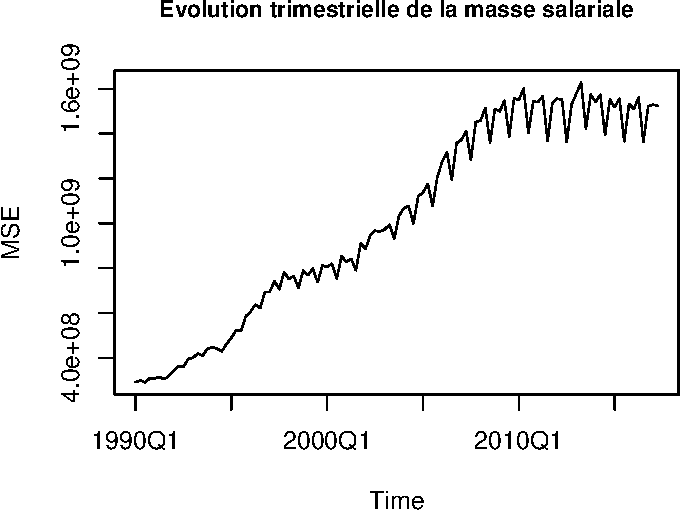
\includegraphics{doc_files/figure-latex/unnamed-chunk-1-1} 

}

\caption{\label{fig1} Evolution trimestrielle de la masse salariale}\label{fig:unnamed-chunk-1}
\end{figure}

La masse salariale trimestrielle, représentée en Figure \ref{fig1}
possède une composante de tendance de 1990 à 2010. La série tend par la
suite à stagner. Nous remarquons également une saisonnalité sur cette
série, qui est de plus en plus marquée à mesure que le temps passe.

\begin{figure}[htbp]
\centering
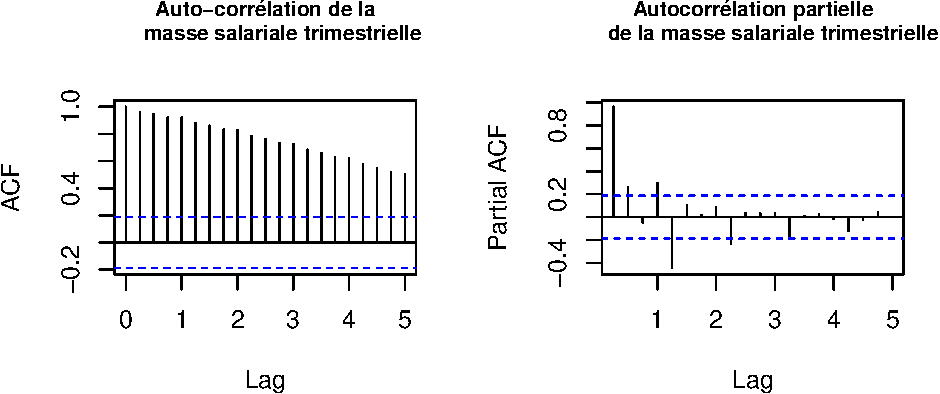
\includegraphics{doc_files/figure-latex/unnamed-chunk-2-1.pdf}
\caption{\label{fig2} Fonctions d'autocorrélation de la masse salariale
trimestrielle}
\end{figure}

\begin{verbatim}
## Warning in kpss.test(MSE): p-value smaller than printed p-value
\end{verbatim}

\begin{verbatim}
## 
##  KPSS Test for Level Stationarity
## 
## data:  MSE
## KPSS Level = 3.6772, Truncation lag parameter = 2, p-value = 0.01
\end{verbatim}

\begin{verbatim}
## Warning in adf.test(MSE): p-value greater than printed p-value
\end{verbatim}

\begin{verbatim}
## 
##  Augmented Dickey-Fuller Test
## 
## data:  MSE
## Dickey-Fuller = -0.20821, Lag order = 4, p-value = 0.99
## alternative hypothesis: stationary
\end{verbatim}

Comme la série comporte une tendance et une saisonnalité, elle ne
correspond pas aux deux premières conditions de la stationnarité du
second ordre, soit que la série possède une moyenne et un écart-type
constants. Cela est confirmé par la Figure \ref{fig2}, qui nous montre
la fonction ACF qui décroît régulièrement. Nous effectuons également un
test de KPSS (test de stationnarité) servant à vérifier si la série est
stationnaire ou non (sous l'hypothèse \(H_{0}\) la série est
stationnaire, et sous l'hypothèse \(H_{1}\) elle ne l'est pas). La série
est dite stationnaire si ses propriétés statistiques (espérance,
variance et auto-corrélation) sont fixes au cours du temps. La p-value
est de 0.01 ce qui nous confirme que la série n'est pas stationnaire
avec un risque de première espèce de 5\%. Nous mettons également en
place un test de racines unitaires, le test de Dickey Fuller augmenté.
Son hypothèse nulle est que la série a été générée par un processus
présentant une racine unitaire, et donc que la série n'est pas
stationnaire. Ici, avec un risque de première espèce à 5\%, on conserve
l'hypothèse nulle et on conclut, à l'aide des deux tests effectués, que
la série n'est pas stationnaire.

\subsection{\texorpdfstring{PIB \label{PIB}}{PIB }}\label{pib}

La Figure \ref{fig3} nous montre l'évolution trimestriel du PIB qui,
comme pour la masse salariale possède une tendance. Cependant, elle ne
semble pas posséder de saisonnalité. Cette série ne semble donc pas non
plus stationnaire. Nous effectuons à nouveau un test de KPSS. La p-value
est de 0.01 ce qui nous confirme que la série n'est pas stationnaire
avec un risque de première espèce de 5\%. Même conclusion au regard du
test augmenté de Dickey Fuller.

\begin{figure}

{\centering 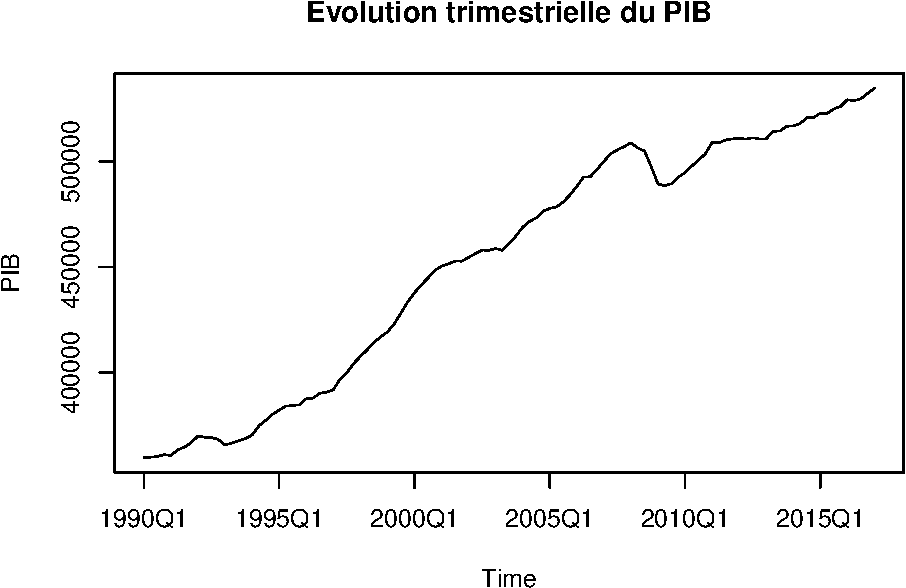
\includegraphics{doc_files/figure-latex/unnamed-chunk-3-1} 

}

\caption{\label{fig3} Evolution trimestrielle du PIB}\label{fig:unnamed-chunk-3}
\end{figure}

\begin{figure}[htbp]
\centering
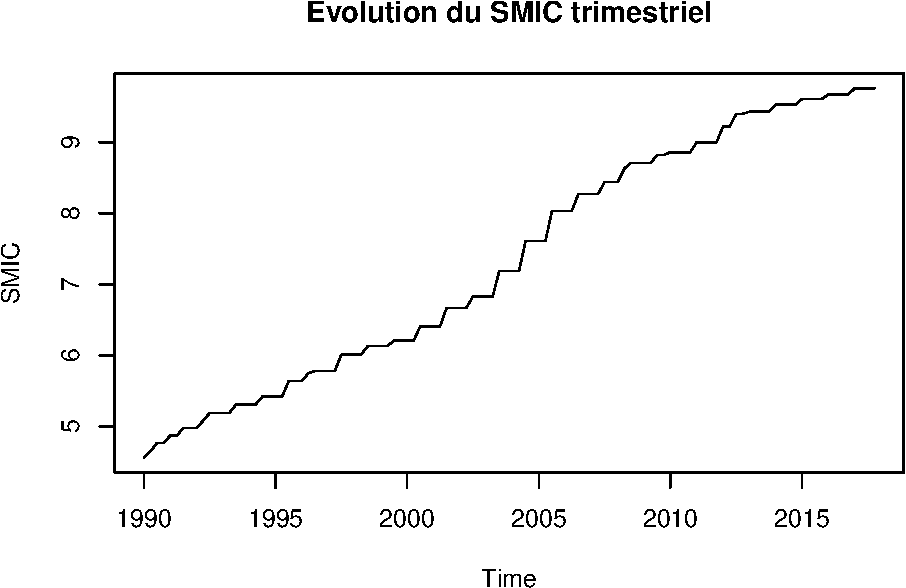
\includegraphics{doc_files/figure-latex/unnamed-chunk-4-1.pdf}
\caption{\label{fig4} ACF et PACF du PIB trimestriel}
\end{figure}

\begin{verbatim}
## Warning in kpss.test(PIB): p-value smaller than printed p-value
\end{verbatim}

\begin{verbatim}
## 
##  KPSS Test for Level Stationarity
## 
## data:  PIB
## KPSS Level = 3.6473, Truncation lag parameter = 2, p-value = 0.01
\end{verbatim}

\begin{verbatim}
## 
##  Augmented Dickey-Fuller Test
## 
## data:  PIB
## Dickey-Fuller = -1.3274, Lag order = 4, p-value = 0.8557
## alternative hypothesis: stationary
\end{verbatim}

\subsection{SMIC}\label{smic}

Au regard de la Figure \ref{fig5}, on s'aperçoit qu'il y a bien une
tendance. Pour la saisonnalité, il est plus difficile de savoir s'il en
existe une ou pas, puisque la série semble augmenter seulement à
certains temps. Les tests de KPSS et de Dickey Fuller augmenté nous
confirment que la série n'est pas stationnaire.

\begin{figure}

{\centering 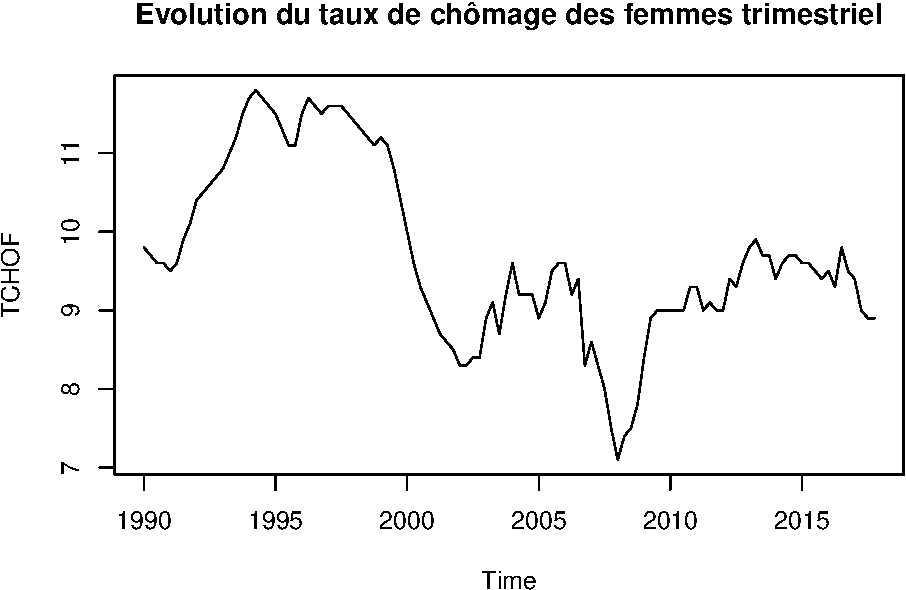
\includegraphics{doc_files/figure-latex/unnamed-chunk-5-1} 

}

\caption{\label{fig5} Evolution trimestrielle du SMIC}\label{fig:unnamed-chunk-5}
\end{figure}

\begin{figure}[htbp]
\centering
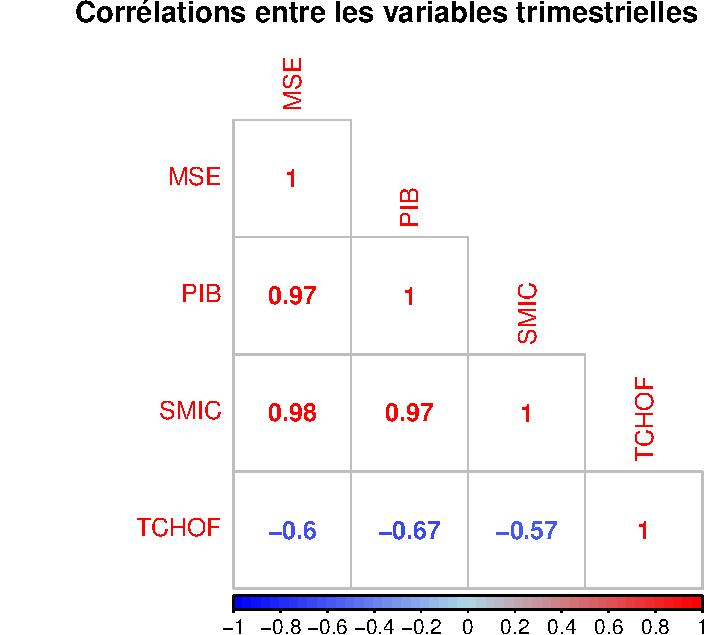
\includegraphics{doc_files/figure-latex/unnamed-chunk-6-1.pdf}
\caption{\label{fig6} ACF et PACF du SMIC trimestriel}
\end{figure}

\begin{verbatim}
## Warning in kpss.test(SMIC): p-value smaller than printed p-value
\end{verbatim}

\begin{verbatim}
## 
##  KPSS Test for Level Stationarity
## 
## data:  SMIC
## KPSS Level = 3.8382, Truncation lag parameter = 2, p-value = 0.01
\end{verbatim}

\begin{verbatim}
## 
##  Augmented Dickey-Fuller Test
## 
## data:  SMIC
## Dickey-Fuller = -1.4174, Lag order = 4, p-value = 0.8184
## alternative hypothesis: stationary
\end{verbatim}

\subsection{\texorpdfstring{Taux de chômage des femmes
\label{TCHOF}}{Taux de chômage des femmes }}\label{taux-de-chomage-des-femmes}

Pour cette dernière série (Figure \ref{fig7}) qui représente le taux de
chômage trimestriel des femmes, il ne semble pas y avoir de
saisonnalité. On remarque cependant qu'il y a bien une tendance, au
regard de la Figure \ref{fig8}. En regardant la série de plus près, on
s'aperçoit que la tendance semble être ``par morceaux'' : d'abord une
hausse de 1990 à 1996, puis elle décroît jusqu'en 2002, avant
d'augmenter à nouveau jusqu'en 2007, de chuter jusqu'en 2010. Si la
série ne possède pas une tendance uniforme sur toute la durée étudiée,
elle semble donc bien posséder une tendance par morceaux. Les tests KPSS
et de Dickey Fuller augmenté nous confirment que la série n'est pas
stationnaire, avec un risque de première espèce de 5\%.

\begin{figure}

{\centering 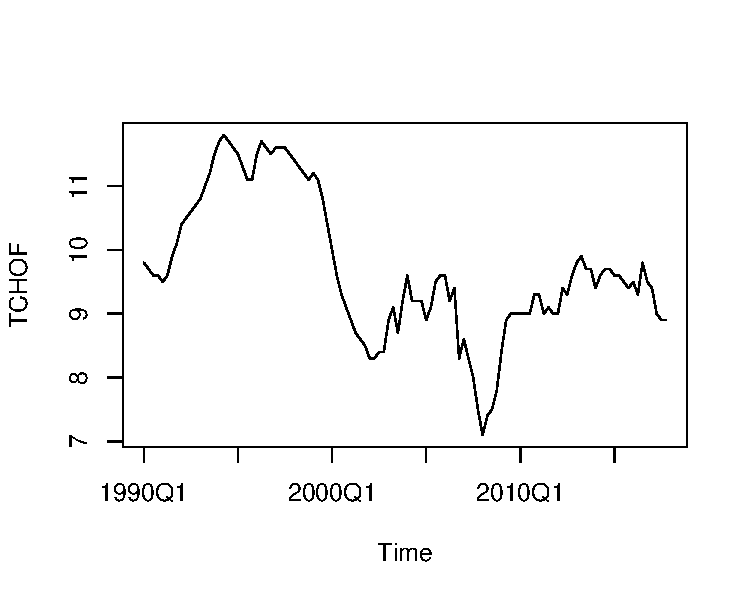
\includegraphics{doc_files/figure-latex/unnamed-chunk-7-1} 

}

\caption{\label{fig7} Evolution trimestrielle du taux de chômage des femmes}\label{fig:unnamed-chunk-7}
\end{figure}

\begin{figure}[htbp]
\centering
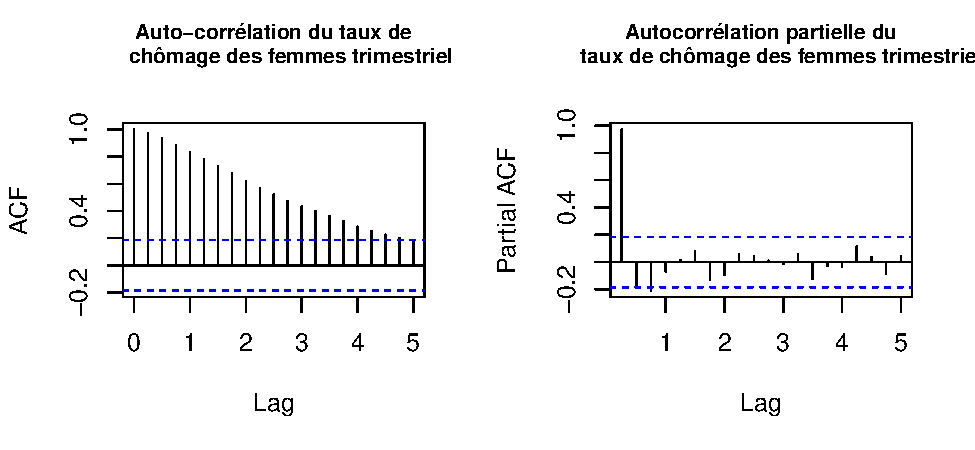
\includegraphics{doc_files/figure-latex/unnamed-chunk-8-1.pdf}
\caption{\label{fig8} ACF et PACF du taux de chômage des femmes
trimestriel}
\end{figure}

\begin{verbatim}
## Warning in kpss.test(TCHOF): p-value smaller than printed p-value
\end{verbatim}

\begin{verbatim}
## 
##  KPSS Test for Level Stationarity
## 
## data:  TCHOF
## KPSS Level = 1.6407, Truncation lag parameter = 2, p-value = 0.01
\end{verbatim}

\begin{verbatim}
## 
##  Augmented Dickey-Fuller Test
## 
## data:  TCHOF
## Dickey-Fuller = -2.5838, Lag order = 4, p-value = 0.3344
## alternative hypothesis: stationary
\end{verbatim}

\subsection{Calcul des corrélations}\label{calcul-des-correlations}

\begin{figure}[htbp]
\centering
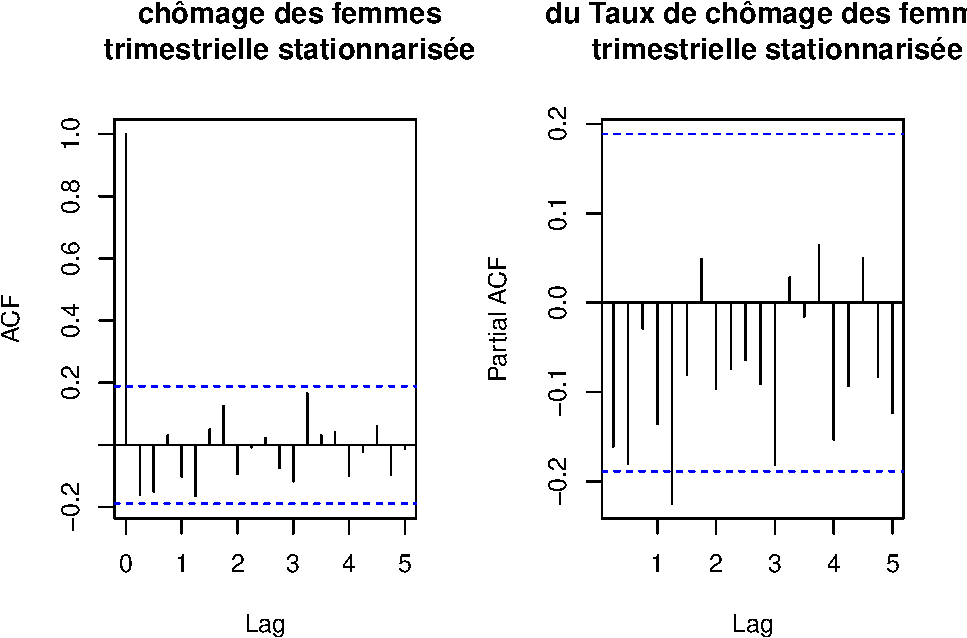
\includegraphics{doc_files/figure-latex/unnamed-chunk-9-1.pdf}
\caption{\label{fig9} Corrélations entre les variables trimestrielles}
\end{figure}

\begin{verbatim}
##                MSE          PIB         SMIC        TCHOF
## MSE   0.000000e+00 3.851955e-69 1.436967e-74 3.321841e-12
## PIB   3.851955e-69 0.000000e+00 1.898200e-71 2.387179e-15
## SMIC  1.436967e-74 1.898200e-71 0.000000e+00 1.377731e-10
## TCHOF 3.321841e-12 2.387179e-15 1.377731e-10 0.000000e+00
\end{verbatim}

Nous affichons la matrice des corrélations des différentes variables en
Figure \ref{fig9}. On se rend compte que le taux de chômage des femmes
est corrélé négativement avec toutes les autres variables. Les variables
PIB, masse salariale et SMIC sont extrêmement liées entre elles. En
regardant le tableau des p-values associées au test de Student (H0 : La
corrélation entre les deux variables est nulle), on s'aperçoit que
toutes les variables prises deux à deux présentes une corrélation.

\subsection{Découpage des séries}\label{decoupage-des-series}

Pour chacune des séries, nous allons créer un échantillon
d'apprentissage, qui nous permettra de construire les différents
modèles, ainsi qu'un échantillon de test, qui nous permettra de comparer
les prédictions des modèles construits avec des vraies valeurs.
L'échantillon d'apprentissage sera composé de toutes les valeurs du
premier trimestre 1990 jusqu'au 4e trimestre 2015, tandis que celui de
test comprendra toutes les valeurs à partir du 1er trimestre 2016.

\subsection{Estimation de la valeur manquante du
PIB}\label{estimation-de-la-valeur-manquante-du-pib}

Contrairement aux autres variables, nous n'avons à notre disposition
pour le PIB que les valeurs jusqu'au premier trimestre de 2017. Ceci
nous impose de négliger la dernière valeur de toutes les autres séries
pour que toutes les variables soient étudiées sur la même période. Pour
éviter ce problème, nous décidons d'estimer la variable du PIB pour le
2e trimestre de 2017. Afin de faire cela, nous allons utiliser la valeur
estimée par un modèle SARIMA correspondant à la variable PIB, étant
donné que c'est celui qui donnait les meilleures prédictions (voir
\ref{Annexe1}).

\newpage

\section{Modélisation vectorielle}\label{modelisation-vectorielle}

Dans la première partie du projet, nous avons modélisé les différentes
séries séparément, à l'aide de modèles de lissage exponentiel ou des
processus ARMA, dont les résultats sont présents en Annexe
\ref{Annexe1}. Nous avons ensuite effectué d'autres modèles ARMA sur la
masse salariale en uilisant les autres variables pour l'expliquer. Ces
modèles sont présents en Annexe \ref{Annexe2}. Cependant, ce type de
modélisation ne nous donne pas de résultats plus performants en terme de
prédictions.

Pendant la deuxième partie du projet, nous nous sommes donc attachés à
utiliser d'autres méthodes de modélisation. Nous nous sommes concentrés
sur les modèles de type vectoriels, qui permettent donc de prédire
plusieurs séries temporelles simultanément. La plus grande partie de nos
travaux portent sur des modèles Vector Auto-Regressive (VAR) plus
quelques tests avec l'ajout d'une partie Moving Average (MA) ce qui nous
donne des modèles VARMA.

\subsection{Définition des modèles}\label{definition-des-modeles}

\subsubsection{Ecriture}\label{ecriture}

Un modèle VAR s'écrit sous la forme suivante :

\(y_t = \sum_{i = 1}^{p} {A_iy_{t-i}} + u_t\)

\(A_i\) représentent les matrices de coefficients du modèle pour un
ordre \(i\) et \(u_t\) une matrice K-dimensionnelle composée des résidus
du modèle (indépendants et identiquement distribués). Enfin, \(p\)
correspond à l'ordre du modèle, qui est en fait le nombre de valeurs du
passé prises en compte pour calculer la valeur présente.

\subsubsection{Hypothèses}\label{hypotheses}

\paragraph{Stabilité du modèle}\label{stabilite-du-modele}

Pour que le modèle soit valide, nous devons vérifier que l'hypothèse de
stabilité est bien respecté. Cette dernière permet d'assurer que les
différentes séries du modèle sont stationnaires. Pour vérifier si un
processus VAR est stable, nous devons calculer les valeurs propres de la
matrice des coefficients suivantes :

\[A = \begin{bmatrix}
A_1 & A_2 & \cdots & A_{p-1} & A_p \\
I & 0 & \cdots & 0 & 0 \\
0 & I & \cdots & 0 & 0 \\
\vdots & \vdots & \ddots & \vdots & \vdots \\
0 & 0 & \cdots & I & 0 
\end{bmatrix}\]

Si les modules des valeurs propres de A sont inférieures à 1, alors le
processus VAR est stable.

\paragraph{Hypothèses sur les résidus}\label{hypotheses-sur-les-residus}

Pour que le modèle soit valide, certaines conditions sur les résidus
doivent également être validées. Il s'agit des suivantes :

\begin{itemize}
\tightlist
\item
  Homoscédasticité
\item
  Normalité
\item
  Absence d'auto-corrélations et de corrélations croisées
\end{itemize}

\subsection{Transformation des séries}\label{transformation-des-series}

Nous allons maintenant transformer les séries pour les rendre
stationnaires, afin de pouvoir appliquer les modèles VAR ensuite. Afin
de stationnariser les séries, nous utiliserons la fonction
\emph{decompose} qui permet de découper la série en trois : la tendance,
la saisonnalité et les résidus, afin de pouvoir ensuite travailler avec
les résidus. Nous ne stationnariserons que les échantillons
d'apprentissage.

\subsubsection{Masse salariale}\label{masse-salariale-1}

\begin{figure}[htbp]
\centering
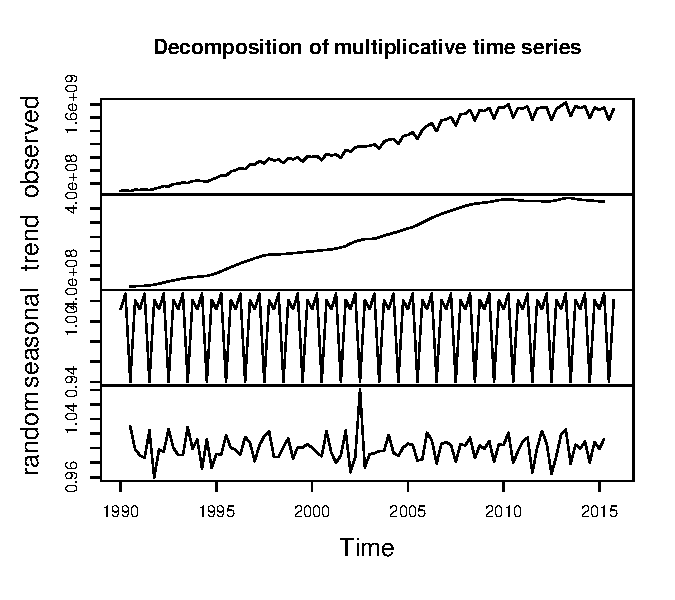
\includegraphics{doc_files/figure-latex/unnamed-chunk-12-1.pdf}
\caption{\label{fig10} Décomposition de la masse salariale}
\end{figure}

Nous nous intéressons aux ACF, PACF (visibles en Figure \ref{fig11}) et
test de KPSS afin de vérifier si les résidus obtenus à l'aide de la
fonction \emph{decompose} sont stationnaires. Bien que l'ACF et la PACF
nous mettent en garde d'une possible non stationnarité de la série, la
p-value des tests de KPSS et Dickey Fuller augmenté nous amène à
confirmer que notre série est désormais stationnarisée (avec un seuil de
confiance à 5\% pour les deux tests effectués).

\begin{figure}[htbp]
\centering
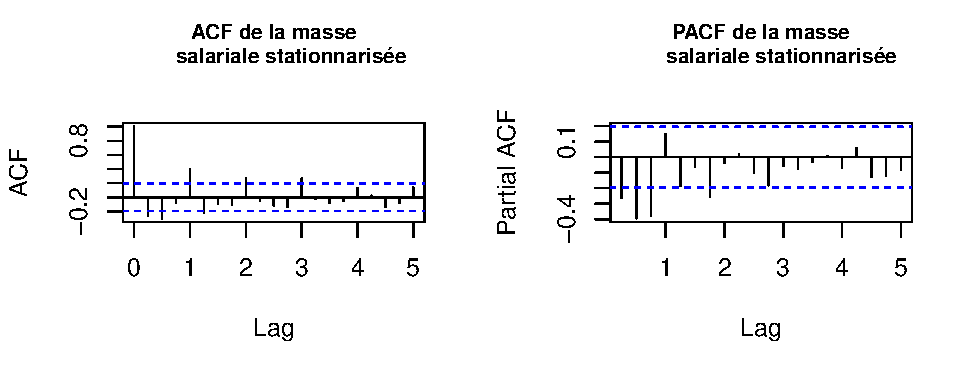
\includegraphics{doc_files/figure-latex/unnamed-chunk-13-1.pdf}
\caption{\label{fig11} Fonctions d'autocorrélation de la masse salariale
stationnarisée}
\end{figure}

\begin{verbatim}
## Warning in kpss.test(MSESta): p-value greater than printed p-value
\end{verbatim}

\begin{verbatim}
## 
##  KPSS Test for Level Stationarity
## 
## data:  MSESta
## KPSS Level = 0.017376, Truncation lag parameter = 2, p-value = 0.1
\end{verbatim}

\begin{verbatim}
## Warning in adf.test(MSESta): p-value smaller than printed p-value
\end{verbatim}

\begin{verbatim}
## 
##  Augmented Dickey-Fuller Test
## 
## data:  MSESta
## Dickey-Fuller = -6.3219, Lag order = 4, p-value = 0.01
## alternative hypothesis: stationary
\end{verbatim}

\begin{figure}[htbp]
\centering
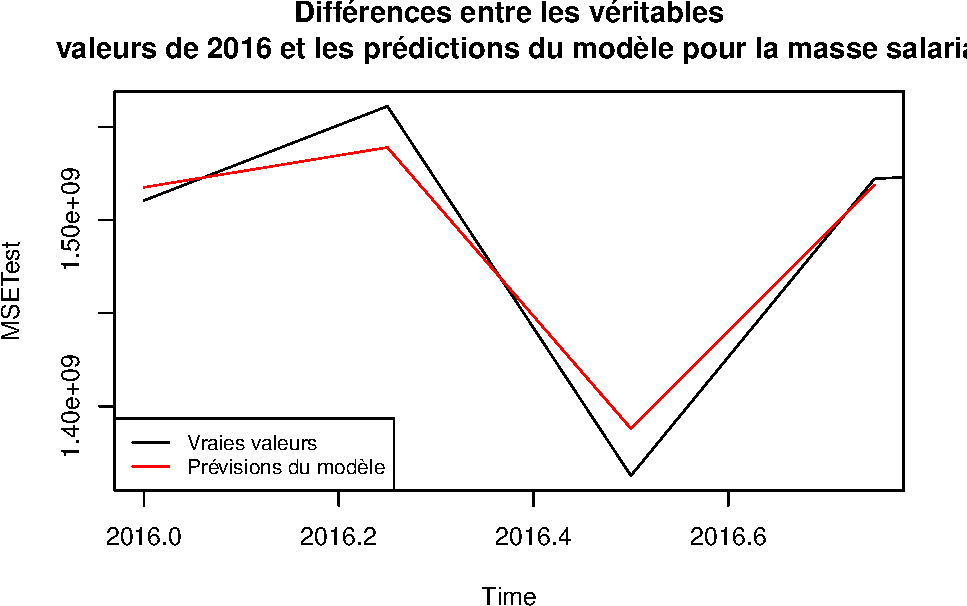
\includegraphics{doc_files/figure-latex/unnamed-chunk-14-1.pdf}
\caption{\label{fig12} Masse salariale trimestrielle stationnarisée}
\end{figure}

\newpage

\subsubsection{PIB}\label{pib-1}

\begin{figure}[htbp]
\centering
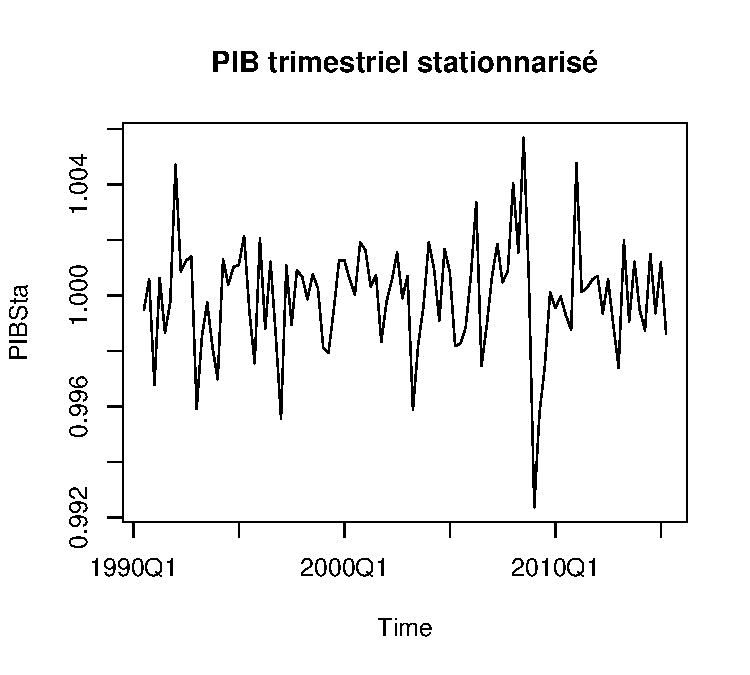
\includegraphics{doc_files/figure-latex/unnamed-chunk-15-1.pdf}
\caption{\label{fig13} PIB trimestriel stationnarisé}
\end{figure}

\begin{figure}[htbp]
\centering
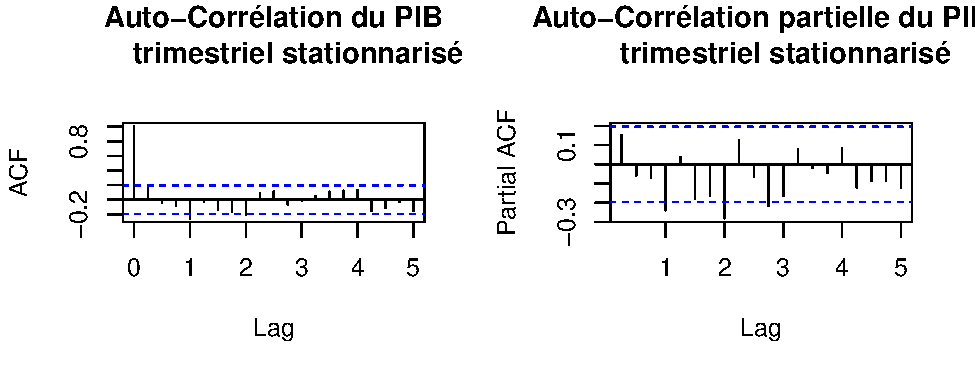
\includegraphics{doc_files/figure-latex/unnamed-chunk-16-1.pdf}
\caption{\label{fig14} Fonctions d'autocorrélation du PIB stationnarisé}
\end{figure}

\begin{verbatim}
## Warning in kpss.test(PIBSta): p-value greater than printed p-value
\end{verbatim}

\begin{verbatim}
## 
##  KPSS Test for Level Stationarity
## 
## data:  PIBSta
## KPSS Level = 0.027524, Truncation lag parameter = 2, p-value = 0.1
\end{verbatim}

\begin{verbatim}
## Warning in adf.test(PIBSta): p-value smaller than printed p-value
\end{verbatim}

\begin{verbatim}
## 
##  Augmented Dickey-Fuller Test
## 
## data:  PIBSta
## Dickey-Fuller = -5.0084, Lag order = 4, p-value = 0.01
## alternative hypothesis: stationary
\end{verbatim}

Nous nous intéressons aux ACF, PACF, test de KPSS et test de Dickey
Fuller augmenté (Figure \ref{fig12}) afin de vérifier si les résidus
obtenus à l'aide de la fonction \emph{decompose} sont stationnaires. Au
regard de ces différentes informations, nous pouvons conclure à la
stationnarité des résidus.

\subsubsection{SMIC}\label{smic-1}

\begin{figure}[htbp]
\centering
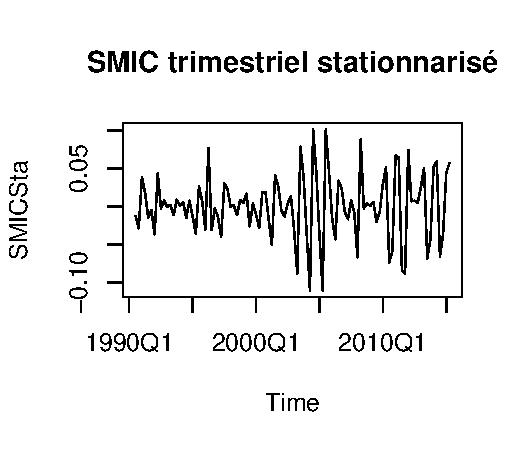
\includegraphics{doc_files/figure-latex/unnamed-chunk-18-1.pdf}
\caption{\label{fig15} SMIC trimestriel stationnarisé}
\end{figure}

Comme pour la masse salariale, les ACF et PACF de la Figure \ref{fig16}
semblent montrer que la série résiduelle pourrait ne pas être
stationnaire. Cependant le test de KPSS ainsi que le test de Dickey
Fuller augmenté nous permettent de conclure à la stationnarité des
résidus.

\begin{figure}[htbp]
\centering
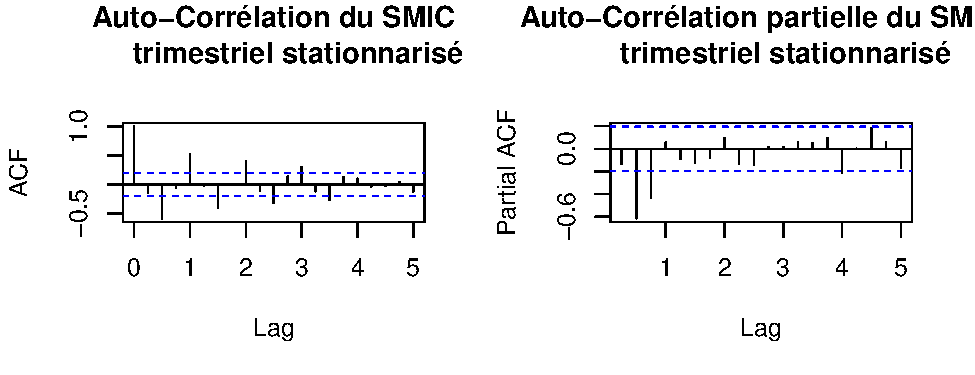
\includegraphics{doc_files/figure-latex/unnamed-chunk-19-1.pdf}
\caption{\label{fig16} Fonctions d'autocorrélation du SMIC
stationnarisé}
\end{figure}

\begin{verbatim}
## Warning in kpss.test(SMICSta): p-value greater than printed p-value
\end{verbatim}

\begin{verbatim}
## 
##  KPSS Test for Level Stationarity
## 
## data:  SMICSta
## KPSS Level = 0.043771, Truncation lag parameter = 2, p-value = 0.1
\end{verbatim}

\begin{verbatim}
## Warning in adf.test(SMICSta): p-value smaller than printed p-value
\end{verbatim}

\begin{verbatim}
## 
##  Augmented Dickey-Fuller Test
## 
## data:  SMICSta
## Dickey-Fuller = -6.357, Lag order = 4, p-value = 0.01
## alternative hypothesis: stationary
\end{verbatim}

\newpage

\subsubsection{Taux de chômage des
femmes}\label{taux-de-chomage-des-femmes-1}

\begin{figure}[htbp]
\centering
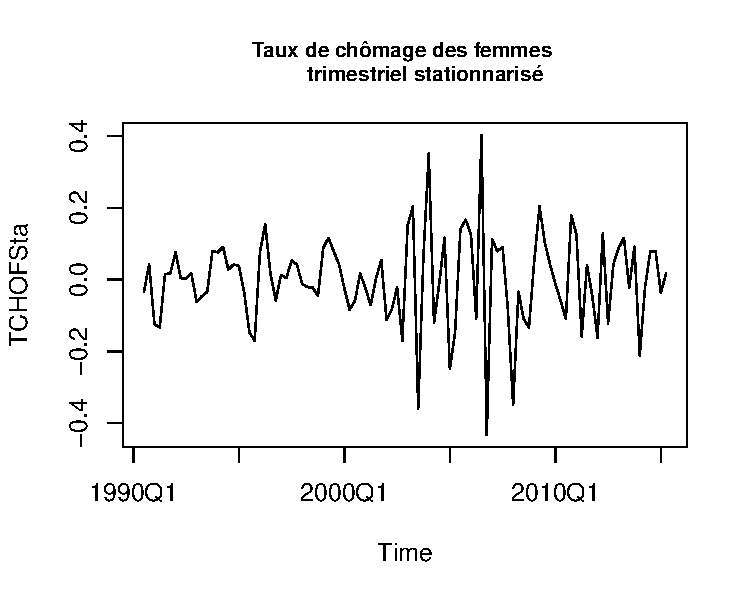
\includegraphics{doc_files/figure-latex/unnamed-chunk-21-1.pdf}
\caption{\label{fig17} Taux de chômage trimestriel stationnarisé}
\end{figure}

En ce qui concerne le taux de chômage des femmes, en regardant l'ACF,
PACF, le test de KPSS et le test de Dickey Fuller augmenté présents en
Figure \ref{fig18}, on peut conclure que la série résiduelle est
stationnaire.

\begin{figure}[htbp]
\centering
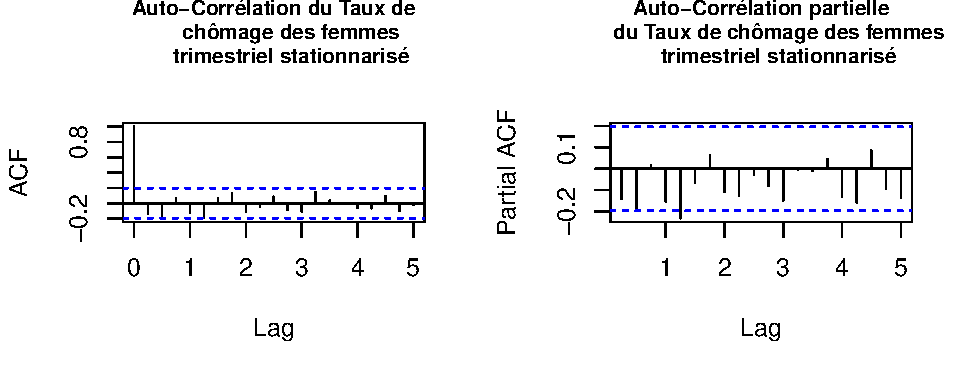
\includegraphics{doc_files/figure-latex/unnamed-chunk-22-1.pdf}
\caption{\label{fig18} Fonctions d'autocorrélation du taux de chômage
stationnarisé}
\end{figure}

\begin{verbatim}
## Warning in kpss.test(TCHOFSta): p-value greater than printed p-value
\end{verbatim}

\begin{verbatim}
## 
##  KPSS Test for Level Stationarity
## 
## data:  TCHOFSta
## KPSS Level = 0.022077, Truncation lag parameter = 2, p-value = 0.1
\end{verbatim}

\begin{verbatim}
## Warning in adf.test(TCHOFSta): p-value smaller than printed p-value
\end{verbatim}

\begin{verbatim}
## 
##  Augmented Dickey-Fuller Test
## 
## data:  TCHOFSta
## Dickey-Fuller = -6.6221, Lag order = 4, p-value = 0.01
## alternative hypothesis: stationary
\end{verbatim}

\newpage

\subsection{Corrélation entre les variables
stationnarisées}\label{correlation-entre-les-variables-stationnarisees}

\begin{figure}[htbp]
\centering
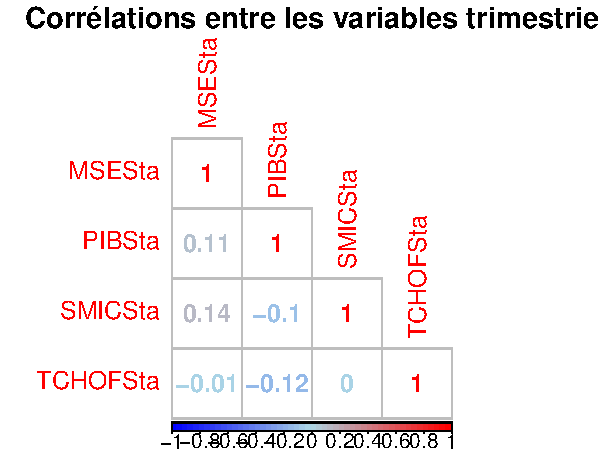
\includegraphics{doc_files/figure-latex/unnamed-chunk-23-1.pdf}
\caption{\label{fig19} Corrélations entre les variables trimestrielles
stationnarisées}
\end{figure}

\begin{verbatim}
##             MSE       PIB      SMIC     TCHOF
## MSE   0.0000000 0.2808591 0.1511096 0.9397487
## PIB   0.2808591 0.0000000 0.3027994 0.2329023
## SMIC  0.1511096 0.3027994 0.0000000 0.9786726
## TCHOF 0.9397487 0.2329023 0.9786726 0.0000000
\end{verbatim}

On s'aperçoit que la transformation de nos séries a permis de supprimer
les corrélations entre elles. En effet, la matrice des corrélations
présentes en Figure \ref{fig19} nous montre que la corrélation la plus
élevée vaut 0.14 ce qui reste très faible. De plus, en regardant le
tableau des p-values, l'hypothèse nulle de non significativité du
coefficient de corrélation n'est rejetée pour aucun couple de variables
(avec un seuil de 5\%).

Maintenant que toutes les séries ont été stationnarisées, elles peuvent
être utilisées pour construire un modèle VAR.

\subsection{Mise en place de modèles VAR avec le package
vars}\label{mise-en-place-de-modeles-var-avec-le-package-vars}

Le package \textbf{vars} a été construit par Bernhard Pfaff (Pfaff
2018). Il permet de construire des modèles vectoriels (VAR), et dispose
également des différentes fonctions de diagnostics permettant de
vérifier que les hypothèses du modèle sont bien remplies. La version
utilisée est la version 1.5-3 et date du 6 Août 2018.

\subsubsection{Calcul de l'ordre p}\label{calcul-de-lordre-p}

Afin de mettre en place une modélisation VAR, nous devons dans un
premier temps nous intéresser à l'ordre p du modèle VAR. L'ordre p
correspond à l'ordre de l'opérateur de retard, c'est-à-dire le nombre de
valeurs du passé qui ont un impact sur la valeur à un instant t. Dans le
package \textbf{vars}, la fonction \emph{VARselect} permet de déterminer
l'ordre des modèles VAR à selectionner en fonction de 4 critères (AIC,
HQ, SC et FPE).

Pour les critères suivants, p correspond à l'ordre du modèle VAR, T le
nombre d'observations utilisées pour la phase d'apprentissage, K le
nombre de variables et
\(\tilde{\Sigma}_u (p) = \frac{1}{T} \Sigma_{t=1}^T \hat{u}_t \hat{u}_t'\)
(la matrice de covariance des résidus du modèle).

Dans cette partie, nous développerons le fonctionement de la
méthodologie en l'appliquant uniquement au modèle complet, soit celui
prenant en compte les variables PIB, SMIC et taux de chômage des femmes.

\begin{figure}[htbp]
\centering
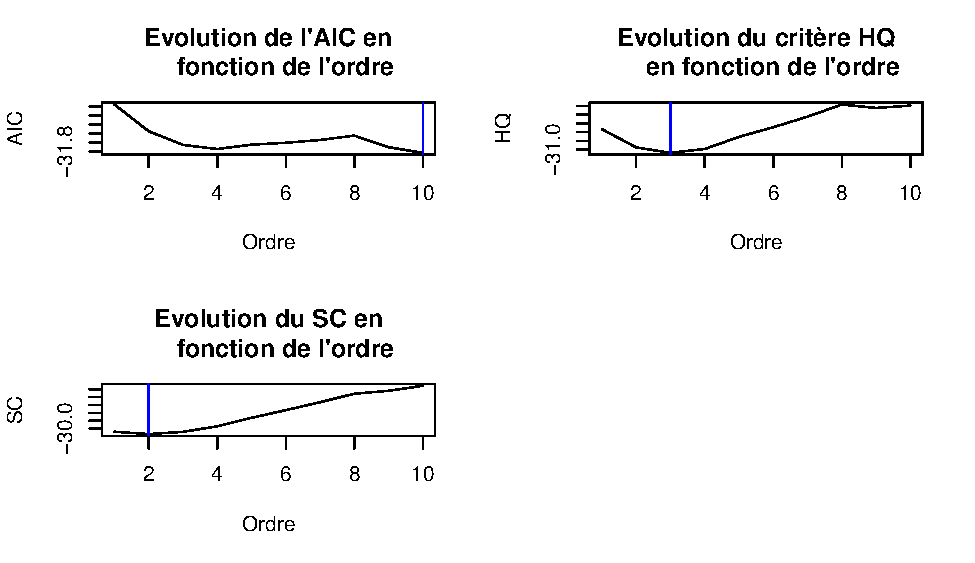
\includegraphics{doc_files/figure-latex/unnamed-chunk-25-1.pdf}
\caption{\label{fig20} Critères associés au modèle complet}
\end{figure}

Le critère AIC (Aikaike information criterion) se calcule, dans ce
package, de la manière suivante :
\(AIC(p) = \ln \det(\tilde{\Sigma}_u(p)) + \frac{2}{T}p K^2 \quad\).
L'objectif est de minimiser ce critère. Cela suppose donc que le
déterminant de la matrice \(\tilde{\Sigma}_u(p)\) soit strictement
positif. Ce critère est asymptotiquement effiace : si le nombre
d'observations tend vers l'infini, sa variance est aussi faible que
possible.

Le critère HQ (Hannan-Quinn criterion) se calcule, dans ce package, de
la manière suivante :
\(HQ(p) = \ln \det(\tilde{\Sigma}_u(p)) + \frac{2 \ln(\ln(T))}{T}p K^2 \quad\).
L'objectif est de minimiser ce critère. Encore une fois, cela suppose
que le déterminant de la matrice \(\tilde{\Sigma}_u(p)\) soit
strictement positif.

Le critère SC (Schwarz criterion) se calcule dans ce package de la
manière suivante :
\(SC(p) = \ln \det(\tilde{\Sigma}_u(p)) + \frac{\ln(T)}{T}p K^2 \quad\).
L'objectif est de minimiser ce critère. Ce critère est un autre nom du
BIC.

On s'aperçoit que les différents critères à notre disposition, visibles
sur les graphiques de la Figure \ref{fig20}, nous donnent des ordres à
choisir différents. Ainsi, le meilleur AIC correspond à un modèle
d'ordre 10, le meilleur HQ à un modèle d'ordre 3 et le meilleur SC à un
modèle d'ordre 2. L'ordre de l'AIC étant trop grand (car trop de
coefficients à estimer par rapport au nombre d'observations à notre
disposition), nous ne souhaitons pas conserver cet ordre. De plus, on se
rend compte que l'AIC du modèle avec un ordre 10 est similaire à celle
d'un modèle avec un ordre 4. Les modèles HQ et SC sont meilleurs avec
respectivement un ordre 3 et 2. Nous allons donc, dans la suite de
l'analyse, essayer les trois modèles définit par les différents critères
: ici, nous allons donc nous intéresser aux modèles d'ordre 2, 3 et 4.

\subsubsection{Estimation du modèle
VAR(p)}\label{estimation-du-modele-varp}

Dans la partie précédente, nous avons sélectionné le meilleur ordre pour
notre modèle VAR. Il s'agit maintenant d'estimer différents modèles afin
de pouvoir prédire la MSE. L'exemple que nous avons pris est pour le
modèle complet, avec les trois ordres déterminés précédemment (2, 3 et
4).

Un modèle VAR s'écrit sous la forme suivante :

\(y_t = \sum_{i = 1}^{p} {A_iy_{t-i}} + u_t\)

\(A_i\) représentent les matrices de coefficients du modèle pour un
ordre i, t le décalage de la série et \(u_t\) une matrice
K-dimensionnelle composée des résidus du modèle (indépendants et
identiquement distribués).

\paragraph{Ordre 4}\label{ordre-4}

Dans le package \textbf{vars}, la fonction utilisée pour construire des
modèles VAR est VAR, qui prend en entrée la série temporelle
multivariée, l'ordre du processus et le type de régresseurs à inclure.
Dans notre cas, \emph{type} vaut \emph{const} car la série est
stationnarisée et donc centrée en une constante \(\mu\). Ci-dessous, le
modèle d'ordre 4.

Les coefficients du modèle sont les suivants. Les erreurs standards
associées sont présentes en Annexe \ref{Annexe3}.

\begin{verbatim}
##               MSE        PIB         SMIC         TCHOF
## MSE   -0.49571073  0.8961454  0.066963585 -0.0127991267
## PIB   -0.03134947  0.1217021 -0.005125468  0.0005912438
## SMIC   0.05931412  1.1813374 -0.496926461 -0.0096012159
## TCHOF -0.88275343 -5.5627534  0.660087437 -0.3220844544
\end{verbatim}

\begin{verbatim}
##               MSE          PIB         SMIC        TCHOF
## MSE   -0.44837936  -0.85710828  0.059065357 -0.016289594
## PIB   -0.03290389  -0.03056789 -0.006426264 -0.001447922
## SMIC  -0.12186822  -0.59050790 -0.674266226 -0.004993847
## TCHOF  0.40185192 -17.96140240  0.821446464 -0.310004540
\end{verbatim}

\begin{verbatim}
##               MSE          PIB        SMIC         TCHOF
## MSE   -0.27254709  -0.67990488  0.04532636  0.0043284001
## PIB   -0.02833629  -0.06107288 -0.01176086 -0.0004898846
## SMIC  -0.27835989  -0.37298995 -0.41721629 -0.0094899806
## TCHOF  0.25697997 -16.67936660  0.63877023 -0.1024043275
\end{verbatim}

\begin{verbatim}
##               MSE        PIB        SMIC        TCHOF
## MSE    0.19486895 -0.4557750  0.09080679 -0.001506479
## PIB   -0.02602058 -0.2762433 -0.00804238  0.001727524
## SMIC   0.14617955  1.3033993  0.08614964 -0.022040339
## TCHOF -1.24236337 -2.7851730  1.22452627 -0.152158590
\end{verbatim}

Les indicateurs de qualité du modèle sont présents ci-dessous.

\begin{verbatim}
##        AIC(n)         HQ(n)         SC(n)        FPE(n) 
## -3.174520e+01 -3.098355e+01 -2.985646e+01  1.664221e-14
\end{verbatim}

Enfin, l'erreur quadratique moyenne de ce modèle pour les données
prédites est la suivante :

\begin{verbatim}
## [1] 7.711856e+14
\end{verbatim}

\begin{figure}[htbp]
\centering
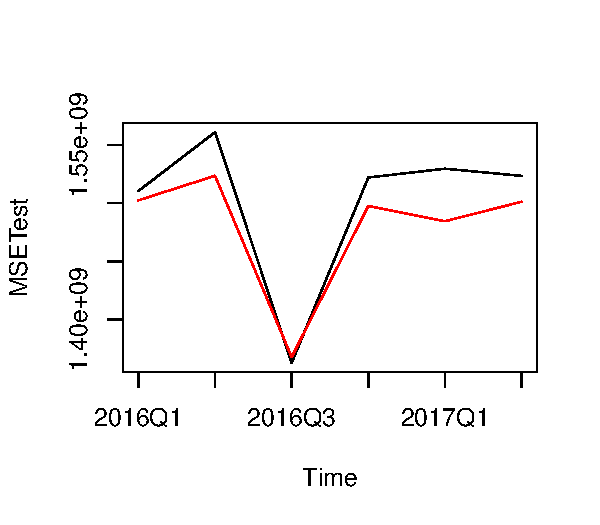
\includegraphics{doc_files/figure-latex/unnamed-chunk-29-1.pdf}
\caption{\label{fig21} Comparaison entre les vraies valeur et le modèle
complet pour un ordre 4}
\end{figure}

La représentation graphique de la Figure \ref{fig21} nous montre des
prédictions proches des vraies valeurs, à part pour le premier trimestre
2017.

\paragraph{Ordre 3}\label{ordre-3}

On s'intéresse ensuite au modèle d'ordre 3, soit celui avec le meilleur
critère HQ.

Les coefficients du modèle associés à un retard de 1 sont les suivants :

\begin{verbatim}
##               MSE        PIB          SMIC        TCHOF
## MSE   -0.55534062  0.5875606  0.0078931593 -0.007157107
## PIB   -0.01712717  0.1810606 -0.0001595774  0.001149490
## SMIC  -0.01904054  0.4355559 -0.5342311296 -0.015680593
## TCHOF -0.40492349 -6.7105659  0.1543612225 -0.278488213
\end{verbatim}

Les indicateurs de qualité du modèle sont présents ci-dessous.

\begin{verbatim}
##        AIC(n)         HQ(n)         SC(n)        FPE(n) 
## -3.165371e+01 -3.107127e+01 -3.020938e+01  1.805099e-14
\end{verbatim}

L'erreur quadratique moyenne de ce modèle pour les données prédites est
la suivante :

\begin{verbatim}
## [1] 9.682886e+14
\end{verbatim}

\begin{figure}[htbp]
\centering
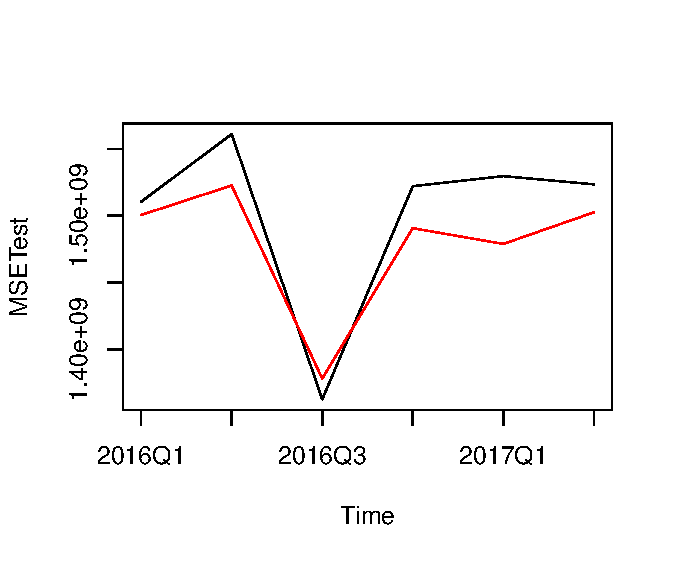
\includegraphics{doc_files/figure-latex/unnamed-chunk-33-1.pdf}
\caption{\label{fig22} Comparaison entre les vraies valeur et le modèle
complet pour un ordre 3}
\end{figure}

Graphiquement, la Figure \ref{fig22} associée à l'ordre 3 nous donne des
prédictions semblant inférieures à celles du modèle d'ordre 4. L'apport
d'un lag supplémentaire dans la construction du retard a donc bien une
importance dans la qualité des prédictions.

\paragraph{Ordre 2}\label{ordre-2}

Enfin, nous construisons le modèle avec le meilleur BIC, soit celui
d'ordre 2.

Les coefficients du modèle associés à un retard de 1 sont les suivants :

\begin{verbatim}
##               MSE        PIB         SMIC        TCHOF
## MSE   -0.39572755  0.8295593  0.030196701 -0.009163581
## PIB   -0.01295909  0.1873301  0.006086945  0.001036053
## SMIC   0.12910889  0.9413863 -0.239926026 -0.022141074
## TCHOF -0.51603938 -6.5905696  0.103373369 -0.217258398
\end{verbatim}

Les indicateurs de qualité du modèle sont présents ci-dessous.

\begin{verbatim}
##        AIC(n)         HQ(n)         SC(n)        FPE(n) 
## -3.135082e+01 -3.094759e+01 -3.035090e+01  2.430391e-14
\end{verbatim}

L'erreur quadratique moyenne de ce modèle pour les données prédites est
la suivante :

\begin{verbatim}
## [1] 9.987686e+14
\end{verbatim}

\begin{figure}[htbp]
\centering
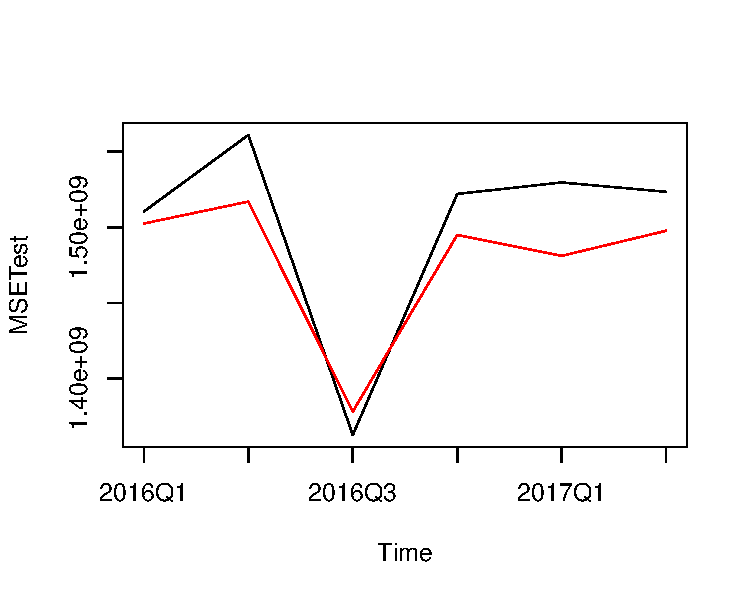
\includegraphics{doc_files/figure-latex/unnamed-chunk-37-1.pdf}
\caption{\label{fig23} Comparaison entre les vraies valeur et le modèle
complet pour un ordre 2}
\end{figure}

Lorsque l'on compare les erreurs quadratiques moyennes, nous remarquons
que la plus faible est celle associée à un modèle d'ordre 4, soit celui
avec le meilleur AIC. Il nous faut maintenant vérifier que les
hypothèses associées à ce modèle soient bien vérifiées.

\subsubsection{Verification de la
stabilité}\label{verification-de-la-stabilite}

Pour vérifier si le processus VAR est stable, c'est-à-dire qu'il génère
des séries stationnaires, nous devons calculer les valeurs propres de la
matrice des coefficients :

\[A = \begin{bmatrix}
A_1 & A_2 & \cdots & A_{p-1} & A_p \\
I & 0 & \cdots & 0 & 0 \\
0 & I & \cdots & 0 & 0 \\
\vdots & \vdots & \ddots & \vdots & \vdots \\
0 & 0 & \cdots & I & 0 
\end{bmatrix}\]

Si les modules des valeurs propres de A sont inférieures à 1, alors le
processus VAR est stable. Nous allons donc vérifier que le processus
VAR(4) créé précédemment avec toutes les variables à notre disposition
est bien stable.

\begin{verbatim}
##  [1] 0.9174340 0.9174340 0.8241534 0.7661190 0.7661190 0.7644083 0.7644083
##  [8] 0.7192911 0.7192911 0.6695288 0.6695288 0.6310697 0.6310697 0.5537349
## [15] 0.4084401 0.2145192
\end{verbatim}

\begin{figure}[htbp]
\centering
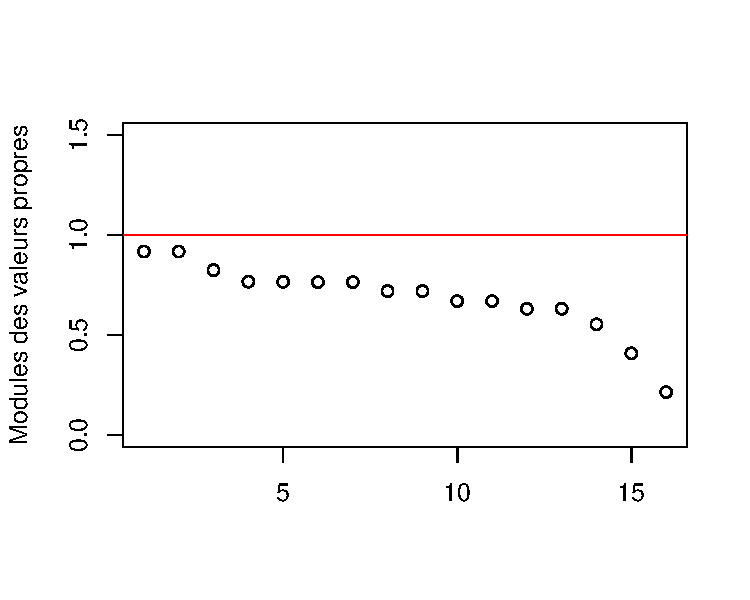
\includegraphics{doc_files/figure-latex/unnamed-chunk-38-1.pdf}
\caption{\label{fig24} Valeurs propres de la matrice A}
\end{figure}

On s'aperçoit que tous les modules sont inférieurs à 1 sur le graphique
de la Figure \ref{fig24}, le processus VAR(4) est donc stable.

\subsubsection{Test ARCH (homoscédasticité des
résidus)}\label{test-arch-homoscedasticite-des-residus}

Le test multivarié de ARCH-LM permet de tester l'homoscédasticité des
résidus. La statistique de test est la suivante :
\(VARCH_{LM}(q) = \frac{1}{2}TK(K+1)R_m^2\), où
\(R_m^2 = 1 - \frac{2}{K(K+1)}tr(\hat{\Omega}\hat{\Omega}_O^{-1})\), et
\(\hat{\Omega}\) est la matrice de covariance de la régression suivante
:
\(vech(\hat{u_t}\hat{u_t}^T) = \beta_0 + B_1 vech(\hat{u}_{t-1}\hat{u}_{t-1}^T) + ... + B_q vech(\hat{u}_{t-q}\hat{u}_{t-q}^T) + v_t\).
La dimension de \(\beta_O\) est \(\frac{1}{2}K(K+1)\) et celle des
matrices des coefficients \(B_i\) est
\(\frac{1}{2}K(K+1) × \frac{1}{2}K(K+1)\). La statistique de test suit
une loi de \(\chi^2(qK^2(K+1)^2/4)\), donc dans notre cas
\(\chi^2(16q*25/4)\). L'hypothèse nulle de ce test est
\(H_0 : B_0 = B_1 = ... = B_q = 0\) (homoscédasticité).

\begin{figure}[htbp]
\centering
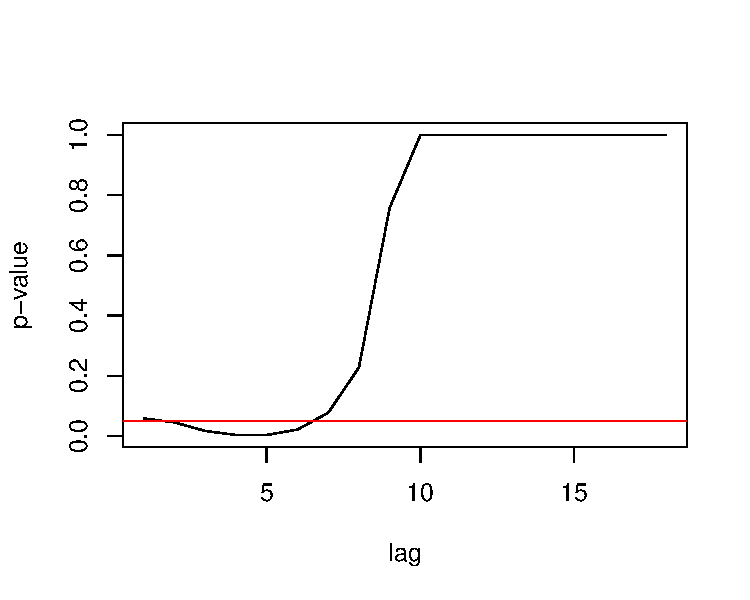
\includegraphics{doc_files/figure-latex/unnamed-chunk-39-1.pdf}
\caption{\label{fig25} Evolution de la p-value en fonction du lag}
\end{figure}

On s'aperçoit au regard de la figure \ref{fig25}, avec un seuil de
confiance de 5\% (ligne rouge), qu'on rejette l'hypothèse nulle
d'homoscédasticité pour un retard faible (inférieur à 7). Cependant, en
augmentant le nombre de valeurs prises en compte pour calculer la
nouvelle, on se rend compte qu'on conserve l'hypothèse
d'homoscédasticité. On observe également que la valeur de la p-value
converge vers 1 au fur et à mesure qu'on augmente le retard. Ainsi, en
prenant l'ensemble des résidus, nous conservons l'hypothèse
d'homoscédasticité.

\subsubsection{Test normalité (normalité des
résidus)}\label{test-normalite-normalite-des-residus}

Le test de Jarque-Bera pour séries multivariées permet de tester la
normalité des résidus. Il utilise les résidus standardisés à l'aide
d'une décomposition de Cholesky de la matrice de variance-covariance des
résidus centrés. Il est important noter que l'ordre dans lequel les
variables sont stockées dans la matrice a une importance sur les
résultats. La statistique de test est la suivante :
\(JB_{mv} = s_3^2 + s_4^2\), où \(s_3^2\) et \(s_4^2\) se calculent de
la sorte : \(s_3^2 = Tb_1^Tb_1/6\) et
\(s_4^2 = T(b_2 - 3_K)^T(b_2-3_K)/24\), avec \(b_1\) et \(b_2\) qui sont
respectivement les vecteurs des moments non-centrés d'ordre trois et
quatre des résidus standardisés. La statistique de test suit une loi de
\(\chi^2(2K)\). Ce test compare en fait le coefficient kurtosis K
(l'aplatissement de la fonction de densité) et le coefficient skewness S
(asymétrie de la fonction de densité) d'une loi normale à ceux des
résidus testés. L'hypothèse nulle est donc \(H0 : S = 0\) et \(K = 3\).

\begin{verbatim}
## 
##  JB-Test (multivariate)
## 
## data:  Residuals of VAR object modele
## Chi-squared = 71.388, df = 8, p-value = 2.599e-12
\end{verbatim}

Ici, on rejette l'hypothèse H0, avec un seuil de confiance de 5\%. Les
résidus obtenus ne suivent pas une loi normale.

\subsubsection{Test Portmanteau (corrélations des
résidus)}\label{test-portmanteau-correlations-des-residus}

Le test de Portmanteau multivarié permet de tester l'auto-corrélation
(au sein d'une même série) et la corrélation croisée (entre les
différentes séries) des résidus.

\paragraph{\texorpdfstring{Verification de la Matrice
\(C_0\)}{Verification de la Matrice C\_0}}\label{verification-de-la-matrice-c_0}

La statistique de Portmanteau est
\(Q_h = T \sum_{j=1}^h tr(\hat{C}_j^T \hat{C}_0^{-1} \hat{C}_j \hat{C}_0^{-1})\),
et elle suit une loi de \(\chi^2(K^2h - n^*)\), \(n^*\) étant le nombre
de coefficients à estimer. Pour qu'elle existe, il faut donc vérifier
que la matrice \(\hat{C}_0\) est inversible pour que la statistique
puisse être définie. Les matrices \(\hat{C}_i\) s'écrivent
\(\hat{C}_i = \frac{1}{T} \sum_{t=i+1}^T \hat{u}_t \hat{u}_{t-i}^T\),
donc \(\hat{C}_0\) s'écrit
\(\hat{C}_0 = \frac{1}{T} \sum_{t=1}^T \hat{u}_t \hat{u}_t^T\). Nous
allons donc vérifier qu'elle est inversible pour le modèle complet que
nous avons mis en place. \(tr()\) correspond à la trace de la matrice,
soit la somme des éléments diagonaux de la matrice.

\begin{verbatim}
##             MSESta        PIBSta       SMICSta      TCHOFSta
## [1,]  1.777427e-04  1.302790e-06  7.666911e-06 -9.660844e-05
## [2,]  1.302790e-06  3.036813e-06 -7.311009e-06 -2.784179e-05
## [3,]  7.666911e-06 -7.311009e-06  7.893080e-04  2.705167e-04
## [4,] -9.660844e-05 -2.784179e-05  2.705167e-04  1.041230e-02
\end{verbatim}

\begin{verbatim}
## Déterminant de la matrice 
##              4.173756e-15
\end{verbatim}

Même si le déterminant est très faible, il n'est pas nul. La matrice
\(\hat{C}_0\) est donc inversible.

\paragraph{Application du test}\label{application-du-test}

Les 3 premières p-values ne peuvent être calculées à cause de la valeur
des degrés de liberté. En effet, comme nous l'avons expliqué plus haut,
la statistique de test suit une loi de \(\chi^2(K^2h - n^*)\). Or, avec
un retard compris entre 1 et 3, les degrés de liberté sont négatifs et
il n'est donc pas possible d'appliquer le test. L'hypothèse nulle de ce
test est l'absence de corrélations croisées et d'auto-corrélations.

\begin{figure}[htbp]
\centering
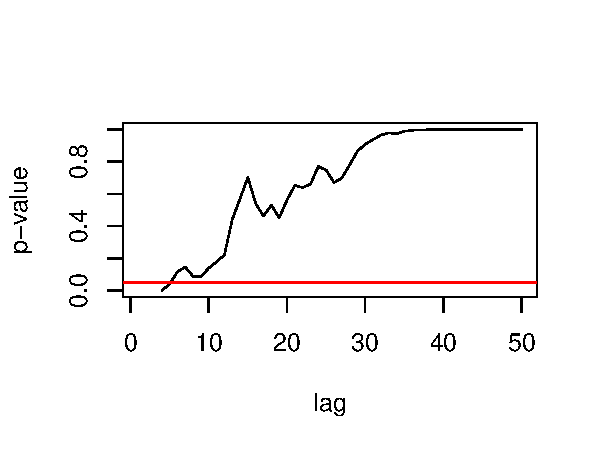
\includegraphics{doc_files/figure-latex/unnamed-chunk-42-1.pdf}
\caption{\label{fig26} Evolution de la p-value en fonction du lag}
\end{figure}

Au regarde la figure \ref{fig26} Comme pour le test ARCH, on rejette
l'hypothèse nulle, avec un seuil de confiance à 5\% (ligne rouge) pour
un retard faible (5 ou moins). Cependant, pour un retard grand
(supérieur à 5), on conserve l'hypothèse nulle d'absence
d'auto-corrélations et de corrélations croisées. On observe également
que la p-value converge vers 1 à mesure qu'on augmente le retard. Ainsi,
en prenant en compte l'ensemble des résidus, on conserve l'hypothèse
d'absence d'auto-corrélations et de corrélations croisées.

\subsubsection{Prévisions}\label{previsions}

Maintenant que nous avons estimé l'ordre des différents modèle VAR, et
que nous avons explicité l'estimation des modèles, nous cherchons
désormais à trouver celui dont les prédictions sont les plus proches de
la réalité.

Après avoir comparé tous les modèles possibles (7 : 3 modèles avec deux
variables, 3 modèles avec trois variables et un modèle avec les quatre
variables), nous nous apercevons que le meilleur en terme de prédictions
est le modèle complet, soit celui que nous avions pris en exemple. Les
AIC et EQM des différents modèles sont résumés dans le tableau
ci-dessous.

\begin{longtable}[]{@{}llll@{}}
\toprule
Variables utilisées & Ordre & AIC & EQM\tabularnewline
\midrule
\endhead
MSE \& PIB & 4 & -20.85328 & 9.153141e+14\tabularnewline
MSE \& SMIC & 3 & -15.37233 & 9.553417e+14\tabularnewline
MSE \& TCHOF & 3 & -12.44526 & 9.880360e+14\tabularnewline
MSE, PIB \& SMIC & 3 & -27.65284 & 9.564856e+14\tabularnewline
MSE, PIB \& TCHOF & 4 & -24.98222 & 9.020987e+14\tabularnewline
MSE, SMIC \& TCHOF & 4 & -19.20940 & 7.955221e+14\tabularnewline
MSE, PIB, SMIC \& TCHOF & 4 & -31.74520 & 7.711856e+14\tabularnewline
\bottomrule
\end{longtable}

\newpage

\subsection{Mise en place de modèles VAR avec le package
MTS}\label{mise-en-place-de-modeles-var-avec-le-package-mts}

Le package \textbf{MTS} a été créé par \textbf{Ruey S. Tsay} and
\textbf{David Wood}, professeurs à l'université de Chicago (Tsay and
Wood 2002). Contrairement au package \textbf{vars}, il ne se limite pas
aux modèles VAR et propose également d'autre types de modèles
multivariés, tels que des modèles de type VMA (Vector Moving Average),
VARMA et même quelques modèles de fonctions de transfert, que nous
n'avons pas eu l'occasion d'étudier. Ce package est très récent, sa
première version datant du 8 octobre 2018.

Pour nous aider à comprendre l'utilisation de ce package, nous nous
somme beaucoup inspirés de l'article \emph{Multivariate Time Series
Analysis with R and Financial Applications} de \textbf{Ruey S.Tsay}

\subsubsection{Calcul de l'ordre p}\label{calcul-de-lordre-p-1}

Afin de mettre en place une modélisation VAR, nous devons dans un
premier temps nous intéresser à l'ordre p du modèle VAR. Dans le package
\textbf{MTS}, la fonction utilisée est VARorder, qui comme VARselect
utilise les critères d'AIC, BIC et HQ afin de déterminer l'ordre du
processus.

Cependant, nous avons également en notre possession un autre critère, la
statistique du test de Tiao-Box ainsi que sa p-value. Ce test évalue
pour un ordre \emph{i} la significativité des coefficients de la matrice
\(A_i\). Ce test permet donc de déterminer si le modèle d'ordre \emph{i}
est meilleur que celui d'ordre \emph{i-1}. La statistique de test est la
suivante :
\(M(i) = -(T-K-i-\frac{3}{2}) \ln(\frac{det(\hat{\Sigma}_1)}{det(\hat{\Sigma}_{i-1})})\),
qui suit une loi du \(\chi^2_{k^2}\). Dans l'exemple que nous prenons,
la première p-value supérieure à 0.05 est celle pour la matrice \(A_5\).
L'ordre que nous devons retenir par rapport à ce test est donc 4.

\begin{verbatim}
## selected order: aic =  10 
## selected order: bic =  0 
## selected order: hq =  3 
## Summary table:  
##        p      AIC      BIC       HQ    M(p) p-value
##  [1,]  0 -30.9791 -30.9791 -30.9791  0.0000  0.0000
##  [2,]  1 -30.8805 -30.4637 -30.7118 18.7080  0.2841
##  [3,]  2 -31.5108 -30.6772 -31.1734 76.5005  0.0000
##  [4,]  3 -31.8493 -30.5988 -31.3432 50.3713  0.0000
##  [5,]  4 -31.9763 -30.3090 -31.3015 32.4105  0.0088
##  [6,]  5 -31.9147 -29.8306 -31.0713 17.7023  0.3416
##  [7,]  6 -31.9083 -29.4074 -30.8962 20.2276  0.2101
##  [8,]  7 -31.8826 -28.9648 -30.7017 17.8005  0.3357
##  [9,]  8 -31.8205 -28.4859 -30.4709 14.5715  0.5562
## [10,]  9 -32.1143 -28.3628 -30.5960 32.2245  0.0093
## [11,] 10 -32.2744 -28.1061 -30.5874 23.2838  0.1064
\end{verbatim}

Comme pour le package VARS, l'AIC associé aux différents modèles diminue
en même temps que l'ordre augmente. Si l'on conserve un ordre
raisonnable, le meilleur AIC est également pour un modèle d'ordre 4. Le
BIC nous donne lui un modèle d'ordre 2 alors que le critère HQ nous
conseille d'utiliser un modèle d'ordre 3. Cela correspond aux mêmes
ordres que ceux données par le package \textbf{vars}.

\subsubsection{Estimation du modèle}\label{estimation-du-modele}

Dans le package \textbf{MTS}, la fonction utilisée pour construire des
modèles VAR est \emph{VAR}, qui prend en entrée la série temporelle
multivariée et l'ordre du processus. On affiche ci-dessous les résultats
renvoyés par la fonction sur le modèle d'ordre 4, soit les coefficients
du modèle pour chaque ordre de retard, les erreurs standard ainsi que
les valeurs des critères de qualité.

\begin{verbatim}
## Constant term: 
## Estimates:  3.117817 1.364744 -1.325939 44.45549 
## Std.Error:  1.664379 0.2175532 3.507354 12.73883 
## AR coefficient matrix 
## AR( 1 )-matrix 
##         [,1]   [,2]     [,3]      [,4]
## [1,] -0.4957  0.896  0.06696 -0.012799
## [2,] -0.0313  0.122 -0.00513  0.000591
## [3,]  0.0593  1.181 -0.49693 -0.009601
## [4,] -0.8828 -5.563  0.66009 -0.322084
## standard error 
##        [,1]  [,2]    [,3]    [,4]
## [1,] 0.1085 0.821 0.05362 0.01345
## [2,] 0.0142 0.107 0.00701 0.00176
## [3,] 0.2287 1.731 0.11300 0.02834
## [4,] 0.8307 6.288 0.41043 0.10293
## AR( 2 )-matrix 
##         [,1]     [,2]     [,3]     [,4]
## [1,] -0.4484  -0.8571  0.05907 -0.01629
## [2,] -0.0329  -0.0306 -0.00643 -0.00145
## [3,] -0.1219  -0.5905 -0.67427 -0.00499
## [4,]  0.4019 -17.9614  0.82145 -0.31000
## standard error 
##        [,1]  [,2]    [,3]    [,4]
## [1,] 0.1180 0.809 0.05463 0.01344
## [2,] 0.0154 0.106 0.00714 0.00176
## [3,] 0.2487 1.704 0.11512 0.02833
## [4,] 0.9034 6.189 0.41811 0.10289
## AR( 3 )-matrix 
##         [,1]     [,2]    [,3]     [,4]
## [1,] -0.2725  -0.6799  0.0453  0.00433
## [2,] -0.0283  -0.0611 -0.0118 -0.00049
## [3,] -0.2784  -0.3730 -0.4172 -0.00949
## [4,]  0.2570 -16.6794  0.6388 -0.10240
## standard error 
##        [,1]  [,2]    [,3]   [,4]
## [1,] 0.1183 0.841 0.05525 0.0130
## [2,] 0.0155 0.110 0.00722 0.0017
## [3,] 0.2493 1.773 0.11643 0.0275
## [4,] 0.9054 6.440 0.42288 0.0998
## AR( 4 )-matrix 
##        [,1]   [,2]     [,3]     [,4]
## [1,]  0.195 -0.456  0.09081 -0.00151
## [2,] -0.026 -0.276 -0.00804  0.00173
## [3,]  0.146  1.303  0.08615 -0.02204
## [4,] -1.242 -2.785  1.22453 -0.15216
## standard error 
##        [,1]  [,2]    [,3]    [,4]
## [1,] 0.1099 0.866 0.05397 0.01239
## [2,] 0.0144 0.113 0.00705 0.00162
## [3,] 0.2315 1.826 0.11372 0.02612
## [4,] 0.8409 6.631 0.41304 0.09486
##   
## Residuals cov-mtx: 
##               [,1]          [,2]          [,3]          [,4]
## [1,]  1.777427e-04  1.302790e-06  7.666911e-06 -9.660844e-05
## [2,]  1.302790e-06  3.036813e-06 -7.311009e-06 -2.784179e-05
## [3,]  7.666911e-06 -7.311009e-06  7.893080e-04  2.705167e-04
## [4,] -9.660844e-05 -2.784179e-05  2.705167e-04  1.041230e-02
##   
## det(SSE) =  4.173756e-15 
## AIC =  -31.82996 
## BIC =  -30.16265 
## HQ  =  -31.15517
\end{verbatim}

Les résultats associés aux modèles d'ordre 3 et 2 sont eux présents en
Annexe \ref{Annexe4} et en Annexe \ref{Annexe5}. Comme pour le package
\textbf{vars}, il nous faut maintenant vérifier les hypothèses du
modèle.

\subsubsection{Vérification des
hypothèses}\label{verification-des-hypotheses}

\paragraph{Vérification de la
stabilité}\label{verification-de-la-stabilite}

Comme pour le package \textbf{vars}, nous vérifions que les modules des
valeurs propres de la matrice A sont tous inférieurs à 1 . R. Tsay
définit cependant la matrice A différemment de B. Pfaff, soit en la
retournant

\[A = \begin{bmatrix}
0 & I & 0 & \cdots & 0 \\
0 & 0 & I & \cdots & 0 \\
\vdots & \vdots & \vdots & \ddots & \vdots \\
0 & 0 & \cdots & 0 & I \\
A_p & A_{p-1} & A_{p-2} & \cdots  & A_1 
\end{bmatrix}\]

\begin{verbatim}
##  [1] 0.9174340 0.9174340 0.8241534 0.7661190 0.7661190 0.7644083 0.7644083
##  [8] 0.7192911 0.7192911 0.6695288 0.6695288 0.6310697 0.6310697 0.5537349
## [15] 0.4084401 0.2145192
\end{verbatim}

\begin{figure}[htbp]
\centering
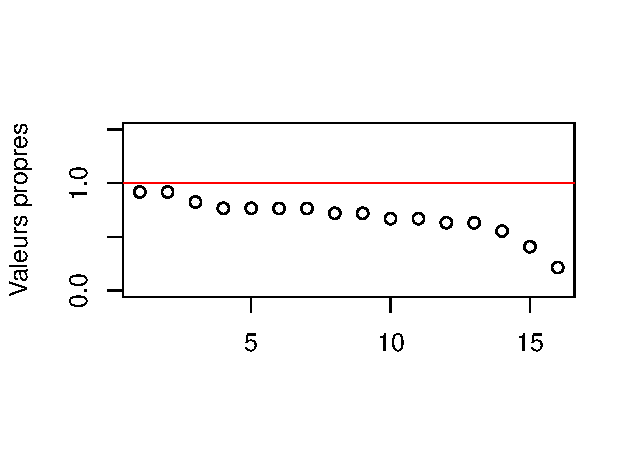
\includegraphics{doc_files/figure-latex/unnamed-chunk-46-1.pdf}
\caption{\label{fig27} Valeurs propres associées à la matrice A}
\end{figure}

La Figure \ref{fig27} nous montre des valeurs propres toutes inférieures
à 1 en module ce qui nous permet de prouver la stabilité du modèle.

\paragraph{Autocorrélation et corrélation
croisée}\label{autocorrelation-et-correlation-croisee}

Nous vérifions ensuite que les résidus ne comportent ni
d'autocorrélation, ni de corrélation croisée. Pour cela, on utilise la
fonction \emph{ccm}, qui vérifie les matrices de corrélation croisée
pour un lag donné. On définit la matrice de variance-covariance pour un
lag \emph{p} comme
\(\hat{\Gamma}_p = \frac{1}{T}\sum_{i=p+1}^{T} (r_t - \bar{r})(r_{t-p} - \bar{r})\).
La matrice de corrélation associée vaut donc
\(\rho_p = \hat{D}^{-1}\hat{\Gamma}_p\hat{D}^{-1}\).

\begin{figure}[htbp]
\centering
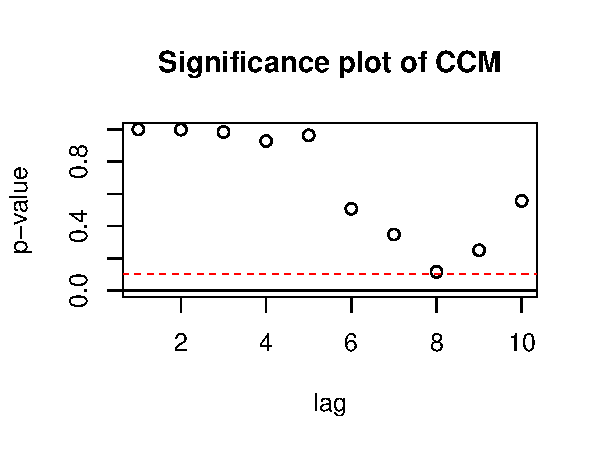
\includegraphics{doc_files/figure-latex/unnamed-chunk-47-1.pdf}
\caption{\label{fig28} Significativité des corrélations croisées pour un
lag de 1 à 10}
\end{figure}

La Figure \ref{fig28} représente le résultat du test d'égalité de la
matrice \(\hat{\Gamma}_p\) à 0. On considère que la corrélation est
significative si elle dépasse le seuil de \(2/\sqrt{T}\) avec T la
longueur de la série. On ne rejette pas l'hypothèse nulle peu importe le
lag, ce qui nous indique que les résidus ne comporte pas de corrélation
croisée.

Nous effectuons ensuite le test de Ljung-Box multivarié, qui teste à la
fois l'autocorrélation et la corrélation croisée. La statistique de ce
test est
\(Q_h = T^2 \sum_{j=1}^h \frac{1}{t-j} tr(\hat{C}_j^T \hat{C}_0^{-1} \hat{C}_j \hat{C}_0^{-1})\),
et elle suit une loi de \(\chi^2(K^2h)\). C'est donc la même statistique
que pour le package \textbf{vars} à un coefficient près.

\begin{verbatim}
## Ljung-Box Statistics:  
##          m       Q(m)     df    p-value
##  [1,]   1.00      1.09   16.00     1.00
##  [2,]   2.00      5.29   32.00     1.00
##  [3,]   3.00     11.75   48.00     1.00
##  [4,]   4.00     20.55   64.00     1.00
##  [5,]   5.00     28.17   80.00     1.00
##  [6,]   6.00     43.72   96.00     1.00
##  [7,]   7.00     61.69  112.00     1.00
##  [8,]   8.00     85.09  128.00     1.00
##  [9,]   9.00    104.85  144.00     0.99
## [10,]  10.00    119.74  160.00     0.99
\end{verbatim}

\begin{figure}[htbp]
\centering
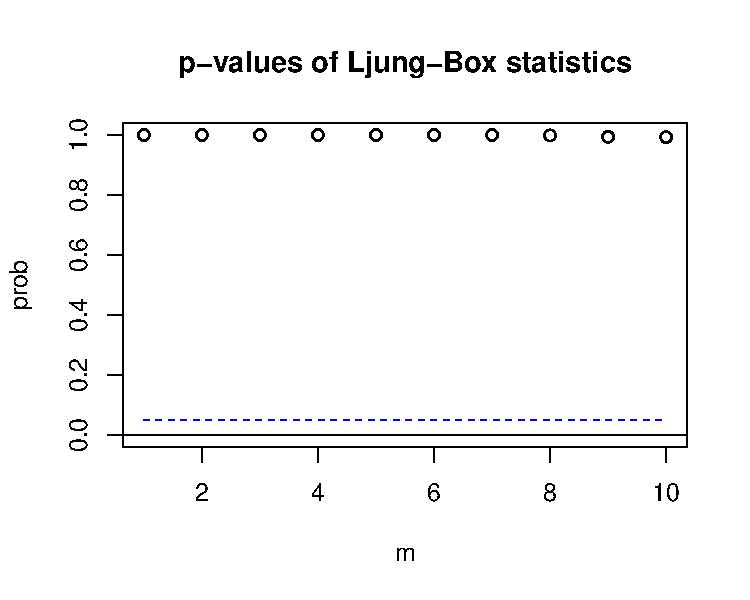
\includegraphics{doc_files/figure-latex/unnamed-chunk-48-1.pdf}
\caption{\label{fig29} Evolution de la p-value en fonction du lag}
\end{figure}

Le résultat de ce test, dont la visualisation graphique est présente
ci-dessus, permet également de conclure que les résidus suivent un bruit
blanc.

\subsubsection{Prévisions}\label{previsions-1}

Comme pour le package précédent, nous résumons dans le tableau suivant
les informations sur les modèles construits. Encore une fois, le plus
performant est le modèle comprenant toutes les variables. On note
également que les EQM obtenues sont identiques à celles du package
\textbf{vars}. Les AIC sont sensiblement les mêmes mais non identiques,
en raison de méthodes de calcul différentes.

\begin{longtable}[]{@{}llll@{}}
\toprule
Variables utilisées & Ordre & AIC & EQM\tabularnewline
\midrule
\endhead
MSE \& PIB & 4 & -20.9333 & 9.153141e+14\tabularnewline
MSE \& SMIC & 3 & -15.4434 & 9.553417e+14\tabularnewline
MSE \& TCHOF & 6 & -12.5389 & 9.880360e+14\tabularnewline
MSE, PIB \& SMIC & 3 & -27.7795 & 9.564856e+14\tabularnewline
MSE, PIB \& TCHOF & 4 & -25.1289 & 9.020987e+14\tabularnewline
MSE, SMIC \& TCHOF & 4 & -19.3573 & 7.955221e+14\tabularnewline
MSE, PIB, SMIC \& TCHOF & 4 & -31.9763 & 7.711856e+14\tabularnewline
\bottomrule
\end{longtable}

\section{Construction de modèles
VARMA}\label{construction-de-modeles-varma}

A la fin du projet, nous avons cherché à ajouter une partie MA à nos
modèles afin d'améliorer les prédictions. Le modèle s'écrit alors de la
façon suivante :

\(y_t = \sum_{i = 1}^{p} {A_iy_{t-i}} + \sum_{i = 1}^{q}{M_iu_{t-i}}\)

On rajoute donc au modèle AR une partie MA représentée par les matrices
\(M_0 ... M_q\). Ce type de modèle n'est que peu utilisé dans la
pratique car il est difficile de satisfaire à la fois les hypothèses
liées à la partie AR et celles liées à la partie MA. On lui préfère donc
souvent un modèle AR, plus simple à construire.

Dans notre cas, la construction de modèle VARMA est possible grâce à la
fonction \emph{VARMA} du package \textbf{MTS}.

\subsection{Calcul des ordres p et q}\label{calcul-des-ordres-p-et-q}

La méthode pour l'estimation des ordres p et q du modèles est un peu
différente de celle pour un modèle VAR. En effet, nous utilisons cette
fois les matrice de corrélation croisée étendues. Si le coefficient
associée à la matrice de corrélation étendue est supérieur au seuil
choisi (5\% pour nous), alors un modèle peut être estimé. La fonction
permettant de complier les matrices de corrélation croisée étendues est
\emph{Eccm}.

\begin{verbatim}
## p-values table of Extended Cross-correlation Matrices: 
## Column: MA order 
## Row   : AR order 
##        0      1      2      3      4      5
## 0 0.0000 0.0000 0.0000 0.0000 0.0053 0.0011
## 1 0.0000 0.0000 0.0000 0.0001 0.0132 0.0380
## 2 0.0376 0.0001 0.0000 0.0364 0.8917 0.9918
## 3 0.7560 0.6384 0.5263 0.9198 0.9927 0.9992
## 4 0.9996 0.8369 0.9676 0.9996 0.9995 0.9763
## 5 1.0000 0.9996 1.0000 1.0000 1.0000 0.9949
\end{verbatim}

Pour le modèle complet, la matrice de corrélation croisée étendue
devient significative à partir d'un modèle VARMA(3,0), soit un modèle
VAR(3). Le but étant de rajouter une partie MA au modèle, les ordres
retenus seront donc 3 et 1.

\subsection{Estimation du modèle}\label{estimation-du-modele-1}

Cependant, les résultats obtenus, présents en Annexe \ref{Annexe6} du
rapport, ne sont pas exploitables. En effet, de nombreux coefficients du
modèles ne sont pas significatifs, potentiellement en raison du grand
nombre de paramètres à estimer. Nous n'avons donc pas réussi à effectuer
des prédictions avec ce modèle.

\newpage

\section{Prévisions sur les années
suivantes}\label{previsions-sur-les-annees-suivantes}

Maintenant que nous avons réalisé nos modèles, vérifié qu'ils
satisfaisaient toutes les hypothèses de construction et comparé les
prédictions de ces modèles aux valeurs de notre échantillon de test,
nous effectuons quelques prédictions pour les années 2018, 2019, 2020 et
2021. Nous utilisons le modèle complet avec un ordre p=4 étant donné que
c'est celui qui donnait les meilleurs résultats.

\begin{verbatim}
##            Qtr1       Qtr2       Qtr3       Qtr4
## 2016 1502432615 1523583648 1367631778 1497596174
## 2017 1484467771 1501242439 1357755499 1480917423
## 2018 1468991799 1485696650 1348625175 1467776769
## 2019 1456214113 1473382375 1340612756 1457418475
## 2020 1445681054 1463727320 1333867818 1449144583
## 2021 1437158372 1455971909 1328199051 1442510992
\end{verbatim}

\begin{figure}[htbp]
\centering
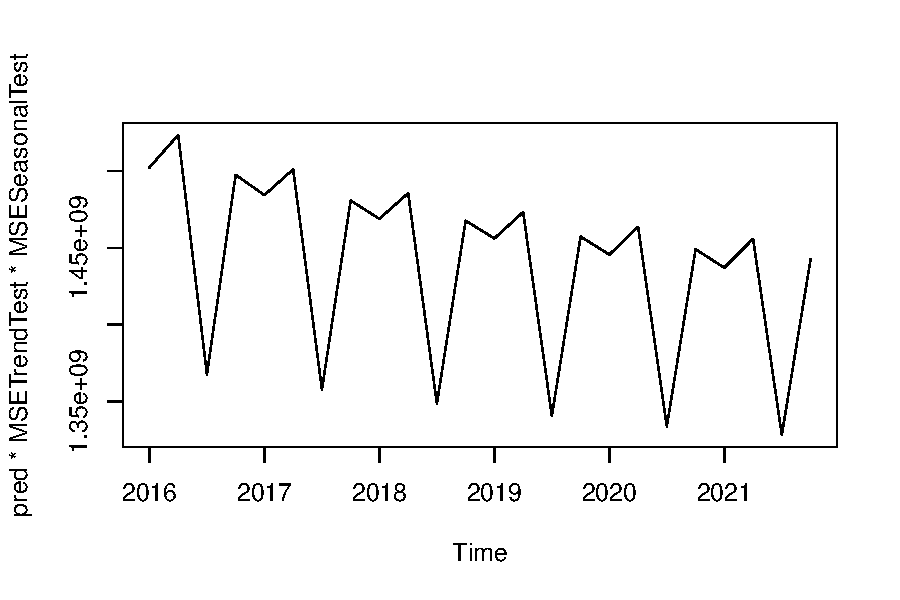
\includegraphics{doc_files/figure-latex/unnamed-chunk-50-1.pdf}
\caption{\label{fig30} Prévisions du modèle VAR pour les années de 2016
à 2021}
\end{figure}

D'après le modèle, la masse salariale devrait baisser dans les années à
venir, d'environ 10 millions chaque année par trimestre. Elle devrait
donc par exemple être d'environ 1.44 milliard d'euros sur le trimestre
prochain.

\newpage

\section*{Conclusion}\label{conclusion}
\addcontentsline{toc}{section}{Conclusion}

Nous avons donc mis en place des modèles de la famille VAR sur le jeu de
données à notre disposition. L'objectif était de regarder si ce type de
modèle pouvait être appliqué en respectant les différents hypothèses
sous-jacentes au modèle, et de regarder la qualité des prédictions du
modèle s'il était possible de le construire.

Afin de mettre en place ce type de modèles, nous avons utilisé deux
packages différents, à savoir vars et MTS, et nous nous rendons compte
que les résultats des deux packages sont similaires.

Nous avons également tenté d'ajouter une composante moyenne-mobile pour
former des modèles VARMA et regarder la qualité de ce type de modèle par
rapport aux modèles VAR que nous avons mis en place. Malheureusement,
les résultats de ces modèles n'étaient pas exploitables

Afin de vérifier si la modélisatio vectorielle est la plus adapté pour
les données de l'IRCEM, il serait bon de comparer ces prédictions avec
des modèles construits à l'aide de fonction de transfert, présents
également dans le package \textbf{MTS}.

\newpage

\appendix

\section{\texorpdfstring{Annexe 1 : Modélisation univariée des séries
\label{Annexe1}}{Annexe 1 : Modélisation univariée des séries }}\label{annexe-1-modelisation-univariee-des-series}

Une fois que nous avons analysé le comportement des différentes séries
temporelles à notre disposition, nous souhaitons les modéliser afin de
prédire les valeurs futures de ces différentes séries. En effet, si nous
voulons prédire la MSE pour des valeurs futures, nous aurons également
besoin des valeurs associées pour les variables explicatives, qui ne
seront peut-être pas à notre disposition. Nous avons utilisé à la fois
des modèles basés sur un lissage exponentiel et des processus ARMA. Nous
nous sommes aidés pour ce faire des travaux de Nicolas Devignes
(Devignes 2018) lors d'un stage au laboratoire Paul Painlevé sur ce
sujet.

\subsection{Comparaison des différents
modèles}\label{comparaison-des-differents-modeles}

Afin de comparer les modèles construits pour chaque série avec les
différentes méthodes, nous calculons l'Erreur Quadratique Moyenne (EQM),
soit les moyennes des différences au carré entre les valeurs de test et
les valeurs prédites par le modèle.

\subsection{Lissage exponentiel}\label{lissage-exponentiel}

\subsubsection{Définition}\label{definition}

Le lissage exponentiel permet de prédire les valeurs d'une série
temporelle en lissant successivement les données à partir d'une valeur
initiale. Plus les observations sont éloignées dans le passé, moins leur
poids est important lors du calcul. Pour une série stationnaire, la
formule de calcul d'une valeur est la suivante :
\(s_t = \alpha y_t + (1-\alpha) s_{t-1}\), le paramètre \(\alpha\) étant
le facteur de lissage. Le nom de cette méthode est un lissage
exponentiel \textbf{simple}. Afin de modéliser les séries possédant une
tendance, nous introduisons un paramètre \(\beta\) permettant de la
prendre en compte, la méthode étant appelée lissage exponentiel
\textbf{double}. Enfin, Holt et Winters ont également modifié la méthode
pour qu'elle puisse modéliser les séries comportant une saisonnalité en
introduisant un paramètre \(\gamma\). Ils ont donné leur nom à cette
méthode, qui est donc un lissage exponentiel de \textbf{Holt-Winters}.

Dans notre cas, nous ne calculons pas nous-mêmes \(\alpha\), \(\beta\)
et \(\gamma\) Ces paramètres sont déterminés automatiquement par la
fonction \emph{ets} du package \textbf{forecast} de façon à optimiser la
qualité de la prédiction. Cette fonction permet également de choisir la
méthode à utiliser, grâce à l'argument model. Afin de mesurer la qualité
de notre modèle, nous avons choisi d'utiliser l'\textbf{AICc} (Akaike
Information Criterion with correction). Le choix de l'AICc par rapport à
l'AIC s'explique par le faible nombre de données que nous possédons par
rapport au nombre de paramètres à estimer. C'est ce critère qui nous
servira par la suite afin de comparer nos différents modèles.
\label{AICc}

Prenons l'exemple de la MSE. Nous avons vu dans la partie \ref{MSE} que
la série possédait une tendance linéaire ainsi qu'une saisonnalité
multiplicative. L'argument model de la fonction *ets** prendra donc la
valeur ``ZAM'', (erreur sélectionnée automatiquement, tendance linéaire,
saisonnalité multiplicative). On peut également remarquer que lorsque
tous les paramètres sont automatiquement sélectionnés (valeur ``ZZZ''),
les paramètres retenus sont les mêmes que ceux que nous avions rentré.

\begin{verbatim}
## ETS(M,A,M) 
## 
## Call:
##  ets(y = MSETrain, model = "ZAM") 
## 
##   Smoothing parameters:
##     alpha = 0.7675 
##     beta  = 0.1111 
##     gamma = 0.2325 
## 
##   Initial states:
##     l = 279219343.2211 
##     b = 12053621.0848 
##     s = 1.0092 0.9655 1.0159 1.0094
## 
##   sigma:  0.0279
## 
##      AIC     AICc      BIC 
## 4031.536 4033.451 4055.336
\end{verbatim}

\begin{figure}

{\centering 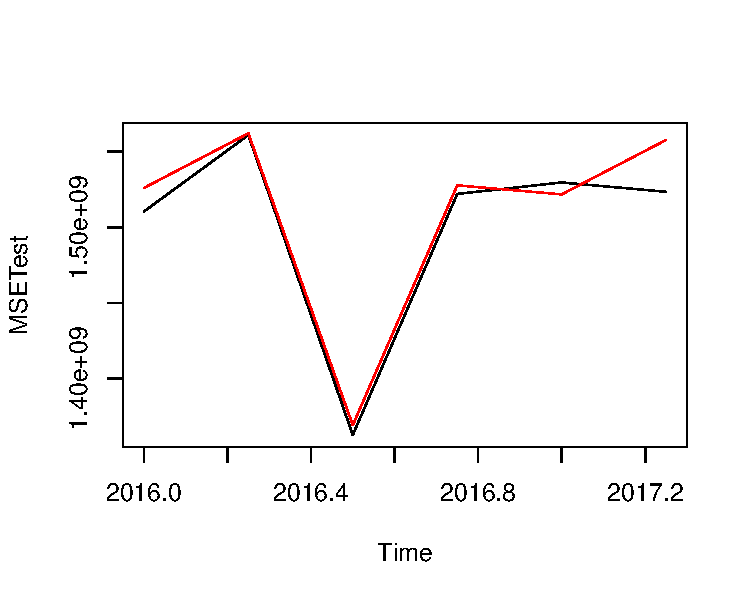
\includegraphics{doc_files/figure-latex/unnamed-chunk-51-1} 

}

\caption{\label{fig31} Comparaison entre la prédiction du lissage exponentiel et les valeurs réelles pour la masse salariale trimestrielle}\label{fig:unnamed-chunk-51}
\end{figure}

\begin{verbatim}
## [1] 2.592281e+14
\end{verbatim}

On obtient donc un AICc de 4033.451 pour le modèle ainsi qu'une erreur
quadratique moyenne de \(2.6*10^{14}\). Le graphique obtenu en figure
\ref{fig31} nous montre que le modèle obtenu nous donne des prédictions
très proches de la réalité.

\subsubsection{Résultats obtenus}\label{resultats-obtenus}

\begin{figure}

{\centering 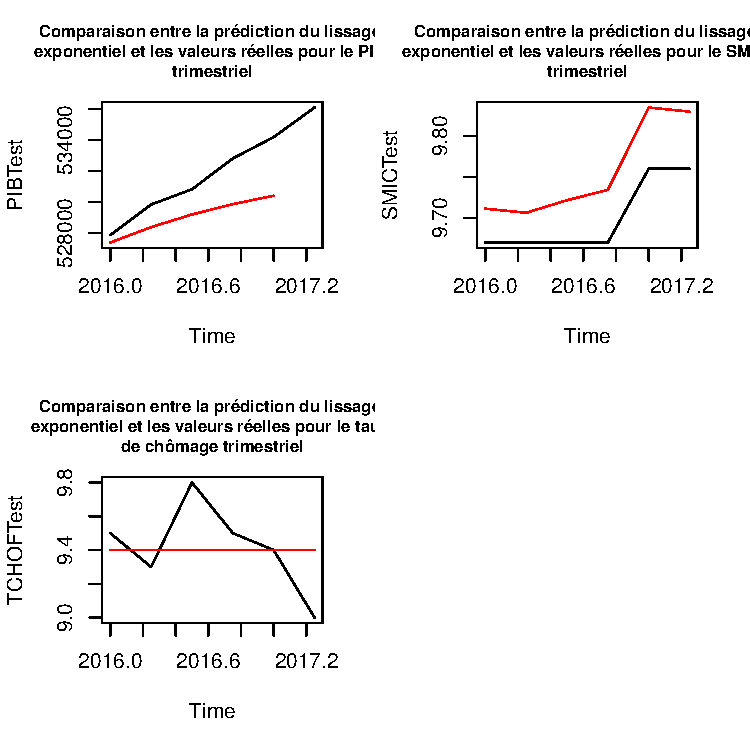
\includegraphics{doc_files/figure-latex/unnamed-chunk-53-1} 

}

\caption{\label{fig32} Résultats obtenus pour le lissage exponentiel}\label{fig:unnamed-chunk-53}
\end{figure}

Les graphiques de la figure \ref{fig32} nous montrent des résultats
mitigés. Pour le PIB et le SMIC, les prédictions suivent la forme de la
série mais en sont éloignées. Pour le taux de chômage des femmes, la
méthode de lissage utilisée est un lissage exponentiel simple, ce qui
nous donne donc des prédictions constantes soit de mauvaise qualité.

Nous résumons dans le tableau suivant les résultats obtenus pour chaque
série estimée par un lissage exponentiel.

\begin{longtable}[]{@{}lllll@{}}
\toprule
Variable & Tendance & Saisonnalité & Argument model & AIC\tabularnewline
\midrule
\endhead
MSE & linéaire & multiplicative & ZAM & 4033.45\tabularnewline
PIB & linéaire & absente & ZAN & 2053.15\tabularnewline
SMIC & linéaire & additive & ZAA & -84.96\tabularnewline
TCHOF & absente & absente & ZNN & 204.37\tabularnewline
\bottomrule
\end{longtable}

\subsection{Modèles ARMA}\label{modeles-arma}

\subsubsection{Définition}\label{definition-1}

Les modèles \textbf{ARMA(p,q)} sont une autre famille de modèles
permettant d'estimer une série temporelle. Il est divisé en deux parties
: une partie autorégressive \textbf{AR} auquel est associé un ordre
\emph{p} qui donne le nombre de valeurs passées qui vont être utiles
dans la prédiction, et une partie moyennes mobiles \textbf{MA} qui
permet de de prendre en compte les \emph{q} innovations de la série dans
le futur.

L'une des propriétés des processus ARMA est qu'ils sont utilisés pour
modéliser des séries stationnaires, donc par extension des séries qui ne
possèdent ni tendance ni saisonnalité. Afin de modéliser des séries non
stationnaires, on généralise les processus ARMA en processus
\textbf{ARIMA(p,d,q)}, \emph{d} représentant l'ordre de différenciation
de la série. Les séries saisonnières sont elles modélisées par des
processus \textbf{\(SARIMA(p ,d, q)(P, D, Q)_s\)} qui modélisent des
séries avec une saisonnalité de période \emph{s}.

Comme pour le lissage exponentiel, nous ne calculons pas nous-mêmes les
ordres des processus. Pour cela, la fonction \emph{auto.arima} du
package \textbf{forecast} nous a été très utile. Elle permet en effet de
trouver les ordres du processus qui optimisent un critère défini à
l'avance et de calculer un modèle avec ces coefficients. Nous avons
choisi d'optimiser l'\textbf{AICc}(Akaike Information Criterion with
correction), pour les raisons évoquées dans la partie \ref{AICc}

\begin{figure}

{\centering 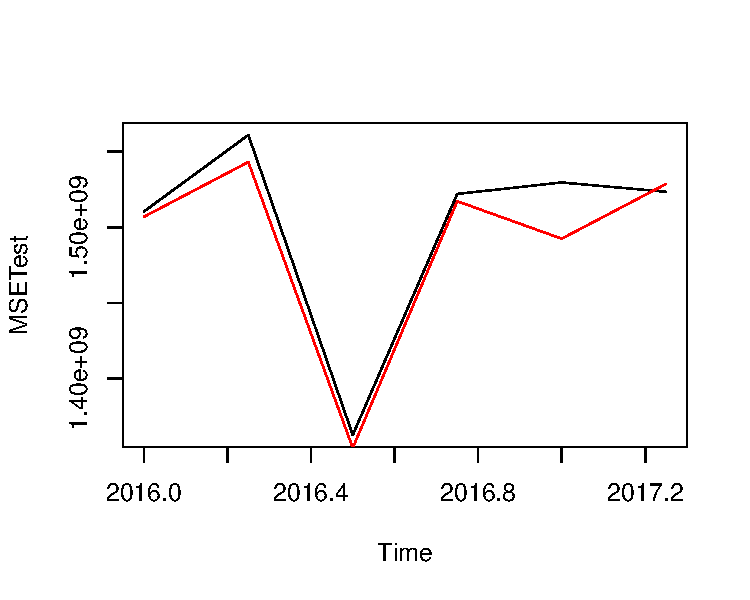
\includegraphics{doc_files/figure-latex/unnamed-chunk-55-1} 

}

\caption{\label{fig33} Comparaison entre le modèle SARIMA et les données de validation pour la masse salariale trimestrielle}\label{fig:unnamed-chunk-55}
\end{figure}

Pour la MSE, on obtient par exemple un modèle \(SARIMA(0,1,1)(0,1,1)_4\)
ainsi qu'un AICc de 3896.01. La figure \ref{fig33} nous donne des
prédictions d'assez bonne qualité mais qui semblent moins bonnes que
celles obtenues par lissage exponentiel.

\subsubsection{Résultats obtenus}\label{resultats-obtenus-1}

\begin{figure}[htbp]
\centering
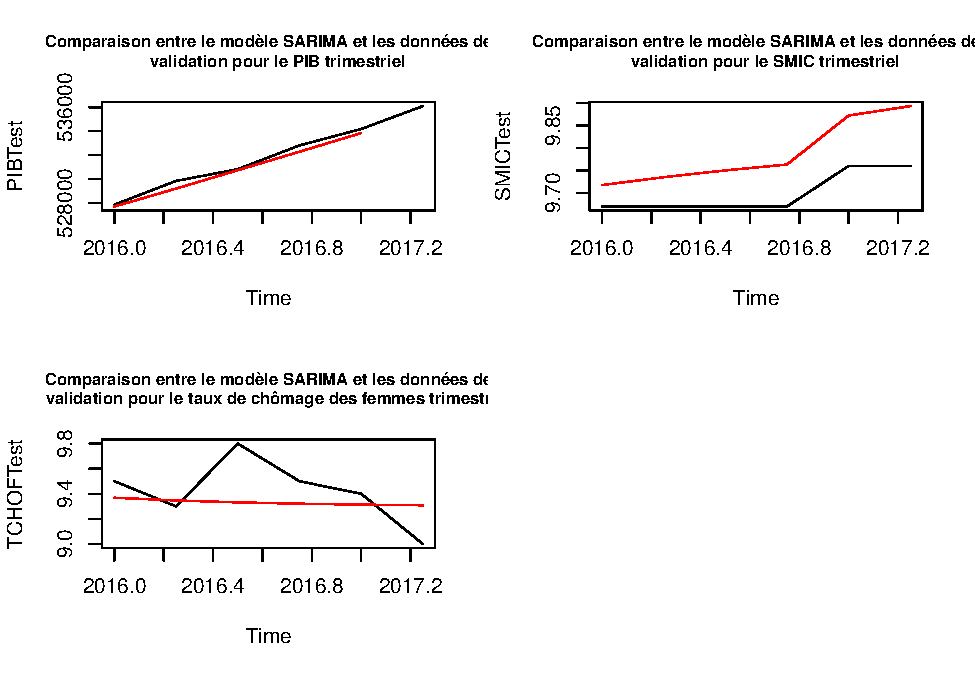
\includegraphics{doc_files/figure-latex/unnamed-chunk-57-1.pdf}
\caption{\label{fig34} Résultats obtenus avec des modèles ARMA}
\end{figure}

Comme pour le lissage exponentiel, nous résumons les résultats obtenus
dans un tableau pour plus de lisibilité. Le PIB et le taux de chômage
des femmes ne comportent pas de partie saisonnière car comme vu dans les
parties \ref{PIB} et \ref{TCHOF} on ne constate pas de saisonnalité dans
l'analyse descriptive de la série. On peut également voir sur la figure
\ref{fig34} que les prédictions du PIB semblent de bien meilleure
qualité

\begin{longtable}[]{@{}lll@{}}
\toprule
Variable & Ordre du processus & AICc\tabularnewline
\midrule
\endhead
MSE & (0,1,1)(0,1,1) & 3675.34\tabularnewline
PIB & (2,1,0) & 1839.36\tabularnewline
SMIC & (1,0,0)(1,1,0) & -261.47\tabularnewline
TCHOF & (0,1,1) & 9.76\tabularnewline
\bottomrule
\end{longtable}

\subsection{Comparaison des différents
modèles}\label{comparaison-des-differents-modeles-1}

Une fois que nous avons construit les deux types de modèles pour chacune
des variables, nous souhaitons les comparer pour savoir quel modèle est
le plus efficace pour prédire chacune des variables. Pour cela, les EQM,
calculant l'erreur de prédiction, de chacun des modèles sont
synthétisées dans le tableau suivant. L'AICc ne peut pas être utilsié
ici car les méthodes à comparer sont différentes. Il n'est donc pas sûr
que la méthode utilisée pour calculer la vraisemblance soit la même.

\begin{verbatim}
##            lissage         ARMA
## MSE   2.592281e+14 3.060118e+14
## PIB   4.654031e+06 1.382004e+05
## SMIC  3.371267e-03 8.609164e-03
## TCHOF 5.833300e-02 6.223076e-02
\end{verbatim}

Nous nous rendons compte que le lissage a une EQM plus faible pour la
masse salariale (notre variable d'intérêt), ainsi que pour le SMIC et le
taux de chômage des femmes. En ce qui concerne le PIB, le modèle ARIMA
est plus performant. Cette analyse va nous servir par la suite, comme
expliqué au début de la partie \ref{Annexe1.1}

\section{\texorpdfstring{Annexe 2 : Modélisation ARMA avec variables
exogènes
\label{Annexe2}}{Annexe 2 : Modélisation ARMA avec variables exogènes }}\label{annexe-2-modelisation-arma-avec-variables-exogenes}

\subsection{Définition}\label{definition-2}

Maintenant que nous avons modélisé chaque série individuellement, nous
souhaitons savoir s'il est possible d'améliorer la qualité de prédiction
de la série MSE trimestrielle à l'aide des autres variables à notre
disposition. Pour ce faire, nous allons construire des modèles SARIMA
prenant en compte des variables exogènes.

\(Y_{t} = \beta_{0} +\beta_{1}X_{1t} + ... + \beta_{k}X_{kt} + \epsilon_{t}\)

\(Y_{t}\) est la variable à modéliser. \(X_{i}\) pour \(i = 1, ..., k\)
correspond à la \(i\)ème variable exogène. \(\beta_{i}\) pour i allant
de \(i = 0, ..., k\) correspond aux coefficients d'une régression
linéaire. Enfin, le résidu \(\epsilon_{t}\) suit un processus de type
ARMA.

\begin{figure}

{\centering 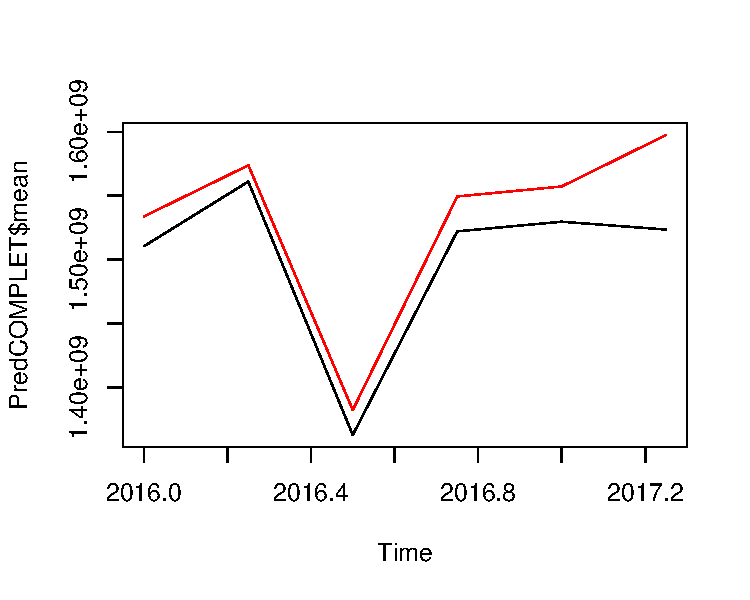
\includegraphics{doc_files/figure-latex/unnamed-chunk-59-1} 

}

\caption{\label{fig35} Masse salariale expliquée par le PIB, le SMIC et le taux de chômage vs Vraies valeurs}\label{fig:unnamed-chunk-59}
\end{figure}

\begin{verbatim}
## [1] 1.345414e+15
\end{verbatim}

Ici, les résidus suivent un SARIMA(0,0,0)(0,1,0){[}4{]}, et le modèle
possède 3 variables exogènes : le coefficient correspondant à la
variable PIB est \(\beta_1 = 706.0045\), celui correspondant à la
variable SMIC est \(\beta_2 = 209266766\) et enfin celui correspondant
au taux de chômage est \(\beta_3 = -1644706\)

\subsection{Résultats obtenus}\label{resultats-obtenus-2}

Nous allons désormais nous intéresser à la construction des différents
modèles prenant en compte 1 variable exogène (3 modèles), 2 variables
exogènes (3 modèles) et 3 variables exogènes (1 modèle). La qualité de
ces 7 modèles est representée dans le tableau ci-dessous.

\begin{longtable}[]{@{}lll@{}}
\toprule
Variable & Ordre du processus & AICc\tabularnewline
\midrule
\endhead
Aucune & (0,1,1)(0,1,1) & 3675.34\tabularnewline
PIB & (1,0,0)(2,1,0) & 3715.99\tabularnewline
SMIC & (0,1,0)(0,1,0) & 3688.92\tabularnewline
TCHOF & (0,0,0)(1,1,0) & 3809.82\tabularnewline
PIB \& SMIC & (0,0,0)(0,1,0) & 3807.37\tabularnewline
PIB \& TCHOF & (1,0,0)(0,1,0) & 3721.36\tabularnewline
SMIC \& TCHOF & (0,1,0)(0,1,0) & 3690.57\tabularnewline
COMPLET & (0,0,0)(0,1,0) & 3809.5\tabularnewline
\bottomrule
\end{longtable}

On se rend compte qu'aucun modèle ARIMA ne prenant en compte des
variables exogènes n'a une qualité meilleure que celui ne prenant en
compte aucune variable exogène (en comparant les AIC corrigés). Si on
omet le modèle sans variable exogène, le meilleur modèle prenant en
compte au moins une variable exogène est celui prenant en compte le SMIC
(dans la figure \ref{fig36}).

\begin{figure}

{\centering 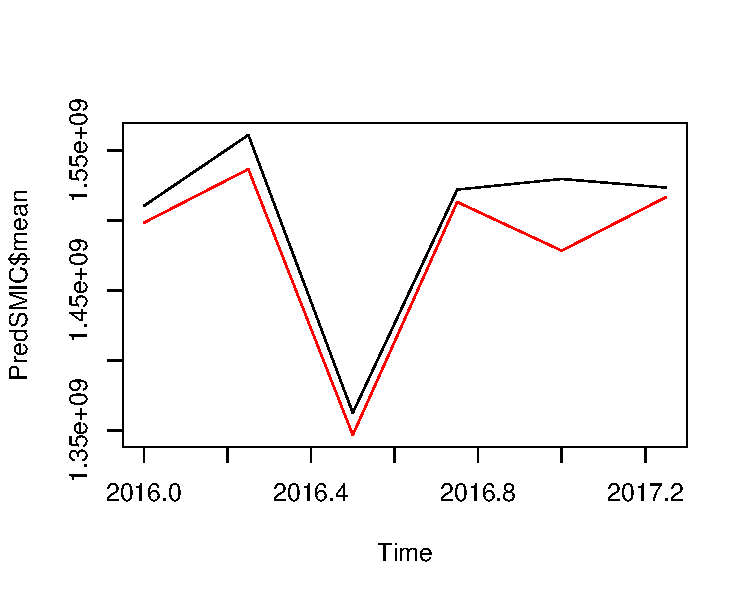
\includegraphics{doc_files/figure-latex/unnamed-chunk-60-1} 

}

\caption{\label{fig36} SARIMA expliqué par le SMIC vs Vraies valeurs}\label{fig:unnamed-chunk-60}
\end{figure}

\begin{verbatim}
## [1] 6.219316e+14
\end{verbatim}

\section{\texorpdfstring{Annexe 3 : Erreurs standard associées aux
coefficients du modèle VAR d'ordre 4
\label{Annexe3}}{Annexe 3 : Erreurs standard associées aux coefficients du modèle VAR d'ordre 4 }}\label{annexe-3-erreurs-standard-associees-aux-coefficients-du-modele-var-dordre-4}

\begin{verbatim}
##               MSE          PIB         SMIC        TCHOF
## MSE   -0.44837936  -0.85710828  0.059065357 -0.016289594
## PIB   -0.03290389  -0.03056789 -0.006426264 -0.001447922
## SMIC  -0.12186822  -0.59050790 -0.674266226 -0.004993847
## TCHOF  0.40185192 -17.96140240  0.821446464 -0.310004540
\end{verbatim}

\begin{verbatim}
##               MSE          PIB        SMIC         TCHOF
## MSE   -0.27254709  -0.67990488  0.04532636  0.0043284001
## PIB   -0.02833629  -0.06107288 -0.01176086 -0.0004898846
## SMIC  -0.27835989  -0.37298995 -0.41721629 -0.0094899806
## TCHOF  0.25697997 -16.67936660  0.63877023 -0.1024043275
\end{verbatim}

\begin{verbatim}
##               MSE        PIB        SMIC        TCHOF
## MSE    0.19486895 -0.4557750  0.09080679 -0.001506479
## PIB   -0.02602058 -0.2762433 -0.00804238  0.001727524
## SMIC   0.14617955  1.3033993  0.08614964 -0.022040339
## TCHOF -1.24236337 -2.7851730  1.22452627 -0.152158590
\end{verbatim}

\section{\texorpdfstring{Annexe 4 : Résultats obtenus pour un modèle VAR
d'ordre 3 pour le modèle complet avec le package MTS
\label{Annexe4}}{Annexe 4 : Résultats obtenus pour un modèle VAR d'ordre 3 pour le modèle complet avec le package MTS }}\label{annexe-4-resultats-obtenus-pour-un-modele-var-dordre-3-pour-le-modele-complet-avec-le-package-mts}

\begin{verbatim}
## Loading required package: MTS
\end{verbatim}

\begin{verbatim}
## Warning: package 'MTS' was built under R version 3.4.4
\end{verbatim}

\begin{verbatim}
## 
## Attaching package: 'MTS'
\end{verbatim}

\begin{verbatim}
## The following object is masked from 'package:vars':
## 
##     VAR
\end{verbatim}

\begin{verbatim}
## Constant term: 
## Estimates:  3.217852 0.9639509 1.007265 36.54962 
## Std.Error:  1.298974 0.1768625 2.680203 10.60551 
## AR coefficient matrix 
## AR( 1 )-matrix 
##         [,1]   [,2]     [,3]     [,4]
## [1,] -0.5553  0.588  0.00789 -0.00716
## [2,] -0.0171  0.181 -0.00016  0.00115
## [3,] -0.0190  0.436 -0.53423 -0.01568
## [4,] -0.4049 -6.711  0.15436 -0.27849
## standard error 
##        [,1]  [,2]    [,3]    [,4]
## [1,] 0.1012 0.791 0.04675 0.01296
## [2,] 0.0138 0.108 0.00636 0.00176
## [3,] 0.2088 1.632 0.09645 0.02674
## [4,] 0.8264 6.458 0.38167 0.10581
## AR( 2 )-matrix 
##         [,1]     [,2]      [,3]      [,4]
## [1,] -0.5372  -0.7716 -0.014791 -0.011517
## [2,] -0.0117  -0.0185 -0.000407 -0.000732
## [3,] -0.2281  -0.4727 -0.739666 -0.003983
## [4,]  1.1588 -17.1794  0.026010 -0.260963
## standard error 
##        [,1] [,2]    [,3]   [,4]
## [1,] 0.1015 0.81 0.03868 0.0125
## [2,] 0.0138 0.11 0.00527 0.0017
## [3,] 0.2095 1.67 0.07982 0.0258
## [4,] 0.8290 6.61 0.31584 0.1021
## AR( 3 )-matrix 
##          [,1]     [,2]     [,3]      [,4]
## [1,] -0.37851  -0.5634 -0.01094  0.004835
## [2,] -0.00979  -0.0879 -0.00835  0.000458
## [3,] -0.33392  -0.3883 -0.45705 -0.013429
## [4,]  0.76852 -14.1815  0.06093 -0.025304
## standard error 
##        [,1]  [,2]   [,3]    [,4]
## [1,] 0.1004 0.839 0.0470 0.01241
## [2,] 0.0137 0.114 0.0064 0.00169
## [3,] 0.2071 1.731 0.0971 0.02560
## [4,] 0.8196 6.848 0.3841 0.10129
##   
## Residuals cov-mtx: 
##               [,1]          [,2]          [,3]          [,4]
## [1,]  1.902501e-04  1.717859e-07  1.508136e-05 -3.048385e-05
## [2,]  1.717859e-07  3.526920e-06 -1.012623e-05 -3.262224e-05
## [3,]  1.508136e-05 -1.012623e-05  8.099521e-04  2.986384e-04
## [4,] -3.048385e-05 -3.262224e-05  2.986384e-04  1.268199e-02
##   
## det(SSE) =  6.444825e-15 
## AIC =  -31.7155 
## BIC =  -30.46502 
## HQ  =  -31.20941
\end{verbatim}

\section{\texorpdfstring{Annexe 5 : Résultats obtenus pour un modèle VAR
d'ordre 2 pour le modèle complet avec le package MTS
\label{Annexe5}}{Annexe 5 : Résultats obtenus pour un modèle VAR d'ordre 2 pour le modèle complet avec le package MTS }}\label{annexe-5-resultats-obtenus-pour-un-modele-var-dordre-2-pour-le-modele-complet-avec-le-package-mts}

\begin{verbatim}
## Constant term: 
## Estimates:  1.923469 0.8755149 0.6145106 24.51231 
## Std.Error:  1.075733 0.1383336 2.345584 8.370214 
## AR coefficient matrix 
## AR( 1 )-matrix 
##        [,1]   [,2]     [,3]     [,4]
## [1,] -0.396  0.830  0.03020 -0.00916
## [2,] -0.013  0.187  0.00609  0.00104
## [3,]  0.129  0.941 -0.23993 -0.02214
## [4,] -0.516 -6.591  0.10337 -0.21726
## standard error 
##        [,1]  [,2]    [,3]    [,4]
## [1,] 0.0977 0.832 0.03839 0.01283
## [2,] 0.0126 0.107 0.00494 0.00165
## [3,] 0.2130 1.815 0.08371 0.02798
## [4,] 0.7601 6.476 0.29873 0.09985
## AR( 2 )-matrix 
##         [,1]     [,2]     [,3]      [,4]
## [1,] -0.3884  -0.9693 -0.02420 -0.005659
## [2,] -0.0123  -0.0376  0.00169 -0.000400
## [3,] -0.1219  -1.5621 -0.64086  0.000695
## [4,]  0.7849 -18.1915  0.03345 -0.225798
## standard error 
##        [,1]  [,2]    [,3]    [,4]
## [1,] 0.0969 0.841 0.03883 0.01272
## [2,] 0.0125 0.108 0.00499 0.00164
## [3,] 0.2112 1.835 0.08467 0.02773
## [4,] 0.7538 6.547 0.30214 0.09896
##   
## Residuals cov-mtx: 
##               [,1]          [,2]          [,3]          [,4]
## [1,]  2.239911e-04  1.481068e-06  5.388294e-05 -6.162593e-05
## [2,]  1.481068e-06  3.704053e-06 -6.133443e-06 -2.671666e-05
## [3,]  5.388294e-05 -6.133443e-06  1.064936e-03  1.240050e-04
## [4,] -6.162593e-05 -2.671666e-05  1.240050e-04  1.356110e-02
##   
## det(SSE) =  1.149382e-14 
## AIC =  -31.45697 
## BIC =  -30.62331 
## HQ  =  -31.11957
\end{verbatim}

\section{\texorpdfstring{Annexe 6 : Résultats obtenus pour un modèle
VARMA(3,1) pour le modèle complet
\label{Annexe6}}{Annexe 6 : Résultats obtenus pour un modèle VARMA(3,1) pour le modèle complet }}\label{annexe-6-resultats-obtenus-pour-un-modele-varma31-pour-le-modele-complet}

\begin{verbatim}
## Number of parameters:  68 
## initial estimates:  4.9726 0.8772 -0.946 43.7282 -0.3981 -0.8484 -0.0838 -0.0103 -0.5111 -0.3454 -0.0336 -0.0163 -0.309 -1.5609 -0.0576 -0.0042 0.0075 0.2934 -0.0014 -7e-04 -0.0038 -0.0721 -4e-04 -0.0013 0.0058 -0.1081 -0.0085 7e-04 -0.1476 3.3556 -0.5666 -0.0135 -0.2257 -1.1414 -0.7742 -0.0093 -0.443 -0.4514 -0.4792 -0.016 0.192 -10.8019 -0.1121 -0.3025 1.6342 -20.4024 -0.0628 -0.2833 1.5446 -15.8918 -0.0903 -0.0395 -0.2573 2.6884 0.1529 -0.0074 -0.0283 -0.2266 0.0028 0.0042 -0.0496 -7.3994 0.1475 -0.0115 -0.9524 -7.0222 0.8913 -0.2155 
## Par. lower-bounds:  2.1854 0.4817 -7.1093 19.5479 -0.7005 -2.7724 -0.1968 -0.04 -0.7174 -1.8945 -0.1034 -0.0392 -0.523 -3.1851 -0.1532 -0.0268 -0.0354 0.0204 -0.0174 -0.0049 -0.033 -0.2919 -0.0103 -0.0045 -0.0246 -0.3385 -0.022 -0.0025 -0.8163 -0.899 -0.8163 -0.0792 -0.682 -4.5669 -0.9285 -0.0599 -0.9162 -4.0429 -0.6907 -0.0659 -2.4314 -27.4937 -1.0917 -0.56 -0.1558 -33.8414 -0.6683 -0.4818 -0.312 -29.9822 -0.9203 -0.2353 -0.6463 -0.3269 -0.0196 -0.056 -0.0835 -0.6544 -0.0217 -0.0027 -0.9099 -14.0673 -0.2341 -0.1189 -4.3275 -33.182 -0.6055 -0.6368 
## Par. upper-bounds:  7.7597 1.2726 5.2174 67.9086 -0.0957 1.0756 0.0291 0.0194 -0.3048 1.2036 0.0362 0.0066 -0.095 0.0632 0.0381 0.0183 0.0504 0.5664 0.0146 0.0035 0.0255 0.1477 0.0095 0.002 0.0362 0.1224 0.0051 0.0039 0.5211 7.6102 -0.3169 0.0521 0.2306 2.2841 -0.6199 0.0413 0.0303 3.1401 -0.2676 0.0339 2.8155 5.8899 0.8675 -0.045 3.4242 -6.9634 0.5427 -0.0848 3.4013 -1.8013 0.7396 0.1563 0.1318 5.7038 0.3255 0.0411 0.0269 0.2013 0.0273 0.0111 0.8107 -0.7314 0.529 0.0958 2.4227 19.1377 2.3881 0.2057 
## Final   Estimates:  4.966752 0.8671174 -0.9442231 43.72315 -0.3979297 -0.8491019 -0.0815316 -0.02464433 -0.5094108 -0.3442084 -0.03305659 -0.01880149 -0.3065709 -1.557941 -0.05937059 0.005288784 -0.011186 0.2801627 0.01284207 -0.003403341 -0.0203592 -0.09598845 -0.0008384281 0.0002298051 0.02834061 -0.04772061 -0.005810614 0.00212954 -0.1471158 3.355913 -0.5690539 -0.009785347 -0.2250566 -1.140614 -0.7716696 -0.01291388 -0.4487308 -0.4569055 -0.4799379 -0.01935663 0.1871509 -10.80671 -0.1120865 -0.3007965 1.628762 -20.40784 -0.06288002 -0.283614 1.540764 -15.89537 -0.09025631 -0.03977166 -0.2471709 2.687042 0.1391174 0.01615111 0.00448665 -0.2186511 -0.02148816 0.003349069 -0.04620208 -7.398882 0.1390584 -0.06520199 -0.9380171 -7.021955 0.9063972 -0.05974413
\end{verbatim}

\begin{verbatim}
## Warning in sqrt(diag(solve(Hessian))): production de NaN
\end{verbatim}

\begin{verbatim}
## 
## Coefficient(s):
##            Estimate  Std. Error  t value Pr(>|t|)    
## MSESta    4.967e+00   7.002e-01    7.093 1.31e-12 ***
## PIBSta    8.671e-01   1.129e-02   76.782  < 2e-16 ***
## SMICSta  -9.442e-01   7.123e-01   -1.326 0.184964    
## TCHOFSta  4.372e+01   6.236e+00    7.011 2.36e-12 ***
## MSESta   -3.979e-01   1.536e-01   -2.590 0.009586 ** 
## PIBSta   -8.491e-01   3.117e-01   -2.724 0.006451 ** 
## SMICSta  -8.153e-02   4.714e-02   -1.730 0.083678 .  
## TCHOFSta -2.464e-02   1.903e-02   -1.295 0.195363    
## MSESta   -5.094e-01   1.204e-01   -4.231 2.33e-05 ***
## PIBSta   -3.442e-01   5.722e-01   -0.602 0.547491    
## SMICSta  -3.306e-02   4.292e-02   -0.770 0.441224    
## TCHOFSta -1.880e-02   1.427e-02   -1.317 0.187744    
## MSESta   -3.066e-01   1.410e-01   -2.174 0.029674 *  
## PIBSta   -1.558e+00   4.696e-01   -3.317 0.000909 ***
## SMICSta  -5.937e-02   5.272e-02   -1.126 0.260080    
## TCHOFSta  5.289e-03   1.423e-02    0.372 0.710211    
## MSESta   -1.119e-02   1.782e-02   -0.628 0.530263    
## PIBSta    2.802e-01   1.332e-02   21.039  < 2e-16 ***
## SMICSta   1.284e-02   8.390e-03    1.531 0.125843    
## TCHOFSta -3.403e-03   2.443e-03   -1.393 0.163656    
## MSESta   -2.036e-02   1.899e-02   -1.072 0.283789    
## PIBSta   -9.599e-02   7.650e-03  -12.548  < 2e-16 ***
## SMICSta  -8.384e-04   7.353e-03   -0.114 0.909222    
## TCHOFSta  2.298e-04   2.377e-03    0.097 0.922988    
## MSESta    2.834e-02   1.667e-02    1.700 0.089136 .  
## PIBSta   -4.772e-02   1.212e-02   -3.938 8.21e-05 ***
## SMICSta  -5.811e-03   7.569e-03   -0.768 0.442701    
## TCHOFSta  2.129e-03   1.953e-03    1.090 0.275512    
## MSESta   -1.471e-01   3.454e-01   -0.426 0.670168    
## PIBSta    3.356e+00          NA       NA       NA    
## SMICSta  -5.691e-01   1.579e-01   -3.604 0.000313 ***
## TCHOFSta -9.785e-03   4.269e-02   -0.229 0.818716    
## MSESta   -2.251e-01   4.090e-01   -0.550 0.582127    
## PIBSta   -1.141e+00   9.042e-01   -1.262 0.207119    
## SMICSta  -7.717e-01   1.521e-01   -5.073 3.91e-07 ***
## TCHOFSta -1.291e-02   4.956e-02   -0.261 0.794440    
## MSESta   -4.487e-01   3.331e-01   -1.347 0.177983    
## PIBSta   -4.569e-01   5.284e-01   -0.865 0.387236    
## SMICSta  -4.799e-01   1.535e-01   -3.127 0.001768 ** 
## TCHOFSta -1.936e-02   4.431e-02   -0.437 0.662211    
## MSESta    1.872e-01   8.303e-01    0.225 0.821671    
## PIBSta   -1.081e+01   3.755e+00   -2.878 0.004005 ** 
## SMICSta  -1.121e-01   3.832e-01   -0.292 0.769910    
## TCHOFSta -3.008e-01   1.154e-01   -2.607 0.009121 ** 
## MSESta    1.629e+00   9.702e-01    1.679 0.093193 .  
## PIBSta   -2.041e+01   4.320e+00   -4.724 2.32e-06 ***
## SMICSta  -6.288e-02   3.689e-01   -0.170 0.864672    
## TCHOFSta -2.836e-01   1.190e-01   -2.383 0.017191 *  
## MSESta    1.541e+00   9.351e-01    1.648 0.099412 .  
## PIBSta   -1.590e+01   3.116e+00   -5.102 3.36e-07 ***
## SMICSta  -9.026e-02   4.114e-01   -0.219 0.826344    
## TCHOFSta -3.977e-02   1.125e-01   -0.354 0.723709    
##          -2.472e-01   1.135e-01   -2.178 0.029423 *  
##           2.687e+00   5.575e-01    4.820 1.44e-06 ***
##           1.391e-01          NA       NA       NA    
##           1.615e-02   1.477e-02    1.093 0.274222    
##           4.487e-03          NA       NA       NA    
##          -2.187e-01   6.839e-02   -3.197 0.001389 ** 
##          -2.149e-02          NA       NA       NA    
##           3.349e-03          NA       NA       NA    
##          -4.620e-02   9.016e-03   -5.124 2.99e-07 ***
##          -7.399e+00          NA       NA       NA    
##           1.391e-01   8.062e-03   17.249  < 2e-16 ***
##          -6.520e-02   4.158e-03  -15.681  < 2e-16 ***
##          -9.380e-01   2.546e-01   -3.684 0.000230 ***
##          -7.022e+00   3.771e+00   -1.862 0.062556 .  
##           9.064e-01          NA       NA       NA    
##          -5.974e-02          NA       NA       NA    
## ---
## Signif. codes:  0 '***' 0.001 '**' 0.01 '*' 0.05 '.' 0.1 ' ' 1
## --- 
## Estimates in matrix form: 
## Constant term:  
## Estimates:  4.966752 0.8671174 -0.9442231 43.72315 
## AR coefficient matrix 
## AR( 1 )-matrix 
##         [,1]    [,2]    [,3]     [,4]
## [1,] -0.3979  -0.849 -0.0815 -0.02464
## [2,] -0.0112   0.280  0.0128 -0.00340
## [3,] -0.1471   3.356 -0.5691 -0.00979
## [4,]  0.1872 -10.807 -0.1121 -0.30080
## AR( 2 )-matrix 
##         [,1]    [,2]      [,3]     [,4]
## [1,] -0.5094  -0.344 -0.033057 -0.01880
## [2,] -0.0204  -0.096 -0.000838  0.00023
## [3,] -0.2251  -1.141 -0.771670 -0.01291
## [4,]  1.6288 -20.408 -0.062880 -0.28361
## AR( 3 )-matrix 
##         [,1]     [,2]     [,3]     [,4]
## [1,] -0.3066  -1.5579 -0.05937  0.00529
## [2,]  0.0283  -0.0477 -0.00581  0.00213
## [3,] -0.4487  -0.4569 -0.47994 -0.01936
## [4,]  1.5408 -15.8954 -0.09026 -0.03977
## MA coefficient matrix 
## MA( 1 )-matrix 
##          [,1]   [,2]    [,3]     [,4]
## [1,]  0.24717 -2.687 -0.1391 -0.01615
## [2,] -0.00449  0.219  0.0215 -0.00335
## [3,]  0.04620  7.399 -0.1391  0.06520
## [4,]  0.93802  7.022 -0.9064  0.05974
##   
## Residuals cov-matrix: 
##               [,1]          [,2]          [,3]          [,4]
## [1,]  2.426715e-04  6.285942e-06 -1.024122e-04 -0.0001170925
## [2,]  6.285942e-06  7.605929e-06 -9.222828e-05 -0.0001004204
## [3,] -1.024122e-04 -9.222828e-05  2.764500e-03  0.0024070658
## [4,] -1.170925e-04 -1.004204e-04  2.407066e-03  0.0159049977
## ---- 
## aic=  -29.47208 
## bic=  -27.70056
\end{verbatim}

\section{Annexe 7 : Code R du projet}\label{annexe-7-code-r-du-projet}

\begin{Shaded}
\begin{Highlighting}[]
\KeywordTok{require}\NormalTok{(tseries)}
\KeywordTok{require}\NormalTok{(forecast)}
\KeywordTok{require}\NormalTok{(corrplot)}
\KeywordTok{require}\NormalTok{(fUnitRoots)}
\KeywordTok{require}\NormalTok{(vars)}


\NormalTok{########################### Importation des données  ######################################}
\NormalTok{trim <-}\StringTok{ }\KeywordTok{read.csv}\NormalTok{(}\StringTok{"~/PFE_Time_Series/Data/Data_Trim.csv"}\NormalTok{, }\DataTypeTok{sep=}\StringTok{";"}\NormalTok{, }\DataTypeTok{dec=}\StringTok{","}\NormalTok{)}
\CommentTok{#trim <- read.csv("~/Cygwin/app/home/Jules/PFE_Time_Series/Data/Data_Trim.csv", sep=";", dec=",")}
\NormalTok{###########################################################################################}

\NormalTok{########################### Analyse descriptive des séries ################################}

\CommentTok{#MSE}
\CommentTok{#Transformation de la masse salariale en série temporelle}
\NormalTok{MSE <-}\StringTok{ }\KeywordTok{ts}\NormalTok{(trim$MSE, }\DataTypeTok{start =} \DecValTok{1990}\NormalTok{, }\DataTypeTok{end =} \KeywordTok{c}\NormalTok{(}\DecValTok{2017}\NormalTok{, }\DecValTok{2}\NormalTok{), }\DataTypeTok{frequency=}\DecValTok{4}\NormalTok{)}
\CommentTok{#Affichage de la série temporelle}
\KeywordTok{plot}\NormalTok{(MSE, }\DataTypeTok{main=}\StringTok{"Evolution trimestrielle de la masse salariale"}\NormalTok{, }\DataTypeTok{xaxt=}\StringTok{"n"}\NormalTok{, }\DataTypeTok{cex.main=}\FloatTok{0.9}\NormalTok{)}
\CommentTok{#Modification de l'axe x pour afficher le nom des trimestres}
\KeywordTok{axis}\NormalTok{(}\DataTypeTok{side=}\DecValTok{1}\NormalTok{, }\DataTypeTok{at=}\KeywordTok{seq}\NormalTok{(}\DecValTok{1990}\NormalTok{,}\DecValTok{2015}\NormalTok{,}\DecValTok{5}\NormalTok{), }\DataTypeTok{labels=}\KeywordTok{c}\NormalTok{(}\StringTok{"1990Q1"}\NormalTok{, }\StringTok{"1995Q1"}\NormalTok{, }\StringTok{"2000Q1"}\NormalTok{, }\StringTok{"2005Q1"}\NormalTok{, }\StringTok{"2010Q1"}\NormalTok{, }\StringTok{"2015Q1"}\NormalTok{))}
\CommentTok{#Division de l'espace d'affichage des graphiques en deux}
\KeywordTok{par}\NormalTok{(}\DataTypeTok{mfrow=}\KeywordTok{c}\NormalTok{(}\DecValTok{1}\NormalTok{,}\DecValTok{2}\NormalTok{), }\DataTypeTok{cex.main=}\FloatTok{0.8}\NormalTok{)}
\CommentTok{#Calcul de l'ACF et des PACF de la masse salariale}
\KeywordTok{acf}\NormalTok{(MSE, }\DataTypeTok{main=}\StringTok{"Auto-corrélation de la masse salariale trimestrielle"}\NormalTok{, }\DataTypeTok{lag.max=}\DecValTok{20}\NormalTok{)}
\KeywordTok{pacf}\NormalTok{(MSE, }\DataTypeTok{main=}\StringTok{"Autocorrélation partielle de la masse salariale trimestrielle"}\NormalTok{, }\DataTypeTok{lag.max=}\DecValTok{20}\NormalTok{)}
\CommentTok{#Réalisation de tests de stationnarité et de racines unitaires}
\KeywordTok{kpss.test}\NormalTok{(MSE)}
\KeywordTok{adf.test}\NormalTok{(MSE)}

\CommentTok{#PIB}
\CommentTok{#Transformation du PIB en série temporelle}
\NormalTok{PIB <-}\StringTok{ }\KeywordTok{ts}\NormalTok{(trim$PIB, }\DataTypeTok{start =} \DecValTok{1990}\NormalTok{, }\DataTypeTok{end =} \KeywordTok{c}\NormalTok{(}\DecValTok{2017}\NormalTok{, }\DecValTok{1}\NormalTok{), }\DataTypeTok{frequency=}\DecValTok{4}\NormalTok{)}
\CommentTok{#Affichage du PIB}
\KeywordTok{plot}\NormalTok{(PIB, }\DataTypeTok{main=}\StringTok{"Evolution trimestrielle du PIB"}\NormalTok{, }\DataTypeTok{xaxt=}\StringTok{"n"}\NormalTok{, }\DataTypeTok{cex.main=}\FloatTok{0.9}\NormalTok{)}
\CommentTok{#Modification de l'axe x}
\KeywordTok{axis}\NormalTok{(}\DataTypeTok{side=}\DecValTok{1}\NormalTok{, }\DataTypeTok{at=}\KeywordTok{seq}\NormalTok{(}\DecValTok{1990}\NormalTok{,}\DecValTok{2015}\NormalTok{,}\DecValTok{5}\NormalTok{), }\DataTypeTok{labels=}\KeywordTok{c}\NormalTok{(}\StringTok{"1990Q1"}\NormalTok{, }\StringTok{"1995Q1"}\NormalTok{, }\StringTok{"2000Q1"}\NormalTok{, }\StringTok{"2005Q1"}\NormalTok{, }\StringTok{"2010Q1"}\NormalTok{, }\StringTok{"2015Q1"}\NormalTok{))}
\CommentTok{#Division de l'espace d'affichage des graphiques en deux}
\KeywordTok{par}\NormalTok{(}\DataTypeTok{mfrow=}\KeywordTok{c}\NormalTok{(}\DecValTok{1}\NormalTok{,}\DecValTok{2}\NormalTok{), }\DataTypeTok{cex.main=}\FloatTok{0.8}\NormalTok{)}
\CommentTok{#Calcul de l'ACF et la PACF du PIB}
\KeywordTok{acf}\NormalTok{(PIB, }\DataTypeTok{main=}\StringTok{"Auto-corrélation du PIB trimestriel"}\NormalTok{, }\DataTypeTok{lag.max=}\DecValTok{40}\NormalTok{)}
\KeywordTok{pacf}\NormalTok{(PIB, }\DataTypeTok{main=}\StringTok{"Autocorrélation partielle du PIB trimestriel"}\NormalTok{, }\DataTypeTok{lag.max=}\DecValTok{40}\NormalTok{)}
\KeywordTok{par}\NormalTok{(}\DataTypeTok{mfrow=}\KeywordTok{c}\NormalTok{(}\DecValTok{1}\NormalTok{,}\DecValTok{1}\NormalTok{))}
\CommentTok{#Réalisation des tests de stationnarité et de racines unitaires}
\KeywordTok{kpss.test}\NormalTok{(PIB)}
\KeywordTok{adf.test}\NormalTok{(PIB)}

\CommentTok{#SMIC}
\CommentTok{#Transformation du SMIC en série temporelle}
\NormalTok{SMIC <-}\StringTok{ }\KeywordTok{ts}\NormalTok{(trim$SMIC, }\DataTypeTok{start =} \KeywordTok{c}\NormalTok{(}\DecValTok{1990}\NormalTok{,}\DecValTok{1}\NormalTok{), }\DataTypeTok{end =} \KeywordTok{c}\NormalTok{(}\DecValTok{2017}\NormalTok{, }\DecValTok{4}\NormalTok{), }\DataTypeTok{frequency =} \DecValTok{4}\NormalTok{)}
\CommentTok{#Affichage du SMIC}
\KeywordTok{plot}\NormalTok{(SMIC, }\DataTypeTok{main=}\StringTok{"Evolution trimestrielle du SMIC"}\NormalTok{, }\DataTypeTok{xaxt=}\StringTok{"n"}\NormalTok{, }\DataTypeTok{cex.main=}\FloatTok{0.9}\NormalTok{)}
\CommentTok{#Modification de l'axe x}
\KeywordTok{axis}\NormalTok{(}\DataTypeTok{side=}\DecValTok{1}\NormalTok{, }\DataTypeTok{at=}\KeywordTok{seq}\NormalTok{(}\DecValTok{1990}\NormalTok{,}\DecValTok{2015}\NormalTok{,}\DecValTok{5}\NormalTok{), }\DataTypeTok{labels=}\KeywordTok{c}\NormalTok{(}\StringTok{"1990Q1"}\NormalTok{, }\StringTok{"1995Q1"}\NormalTok{, }\StringTok{"2000Q1"}\NormalTok{, }\StringTok{"2005Q1"}\NormalTok{, }\StringTok{"2010Q1"}\NormalTok{, }\StringTok{"2015Q1"}\NormalTok{))}
\CommentTok{#Division de l'espace d'affichage des graphiques en deux}
\KeywordTok{par}\NormalTok{(}\DataTypeTok{mfrow=}\KeywordTok{c}\NormalTok{(}\DecValTok{1}\NormalTok{,}\DecValTok{2}\NormalTok{), }\DataTypeTok{cex.main=}\FloatTok{0.8}\NormalTok{)}
\CommentTok{#Calcul de l'ACF et la PACF du SMIC}
\KeywordTok{acf}\NormalTok{(SMIC, }\DataTypeTok{main=}\StringTok{"Auto-corrélation du SMIC trimestriel"}\NormalTok{, }\DataTypeTok{lag.max=}\DecValTok{20}\NormalTok{)}
\KeywordTok{pacf}\NormalTok{(SMIC, }\DataTypeTok{main=}\StringTok{"Autocorrélation partielle du SMIC trimestriel"}\NormalTok{, }\DataTypeTok{lag.max=}\DecValTok{20}\NormalTok{)}
\KeywordTok{par}\NormalTok{(}\DataTypeTok{mfrow=}\KeywordTok{c}\NormalTok{(}\DecValTok{1}\NormalTok{,}\DecValTok{1}\NormalTok{))}
\CommentTok{#Réalisation des tests de stationnarité et de racines unitaires}
\KeywordTok{kpss.test}\NormalTok{(SMIC)}
\KeywordTok{adf.test}\NormalTok{(SMIC)}

\CommentTok{#TCHOF}
\CommentTok{#Création du taux de chômage en série temporelle}
\NormalTok{TCHOF <-}\StringTok{ }\KeywordTok{ts}\NormalTok{(trim$TCHOF, }\DataTypeTok{start =} \KeywordTok{c}\NormalTok{(}\DecValTok{1990}\NormalTok{,}\DecValTok{1}\NormalTok{), }\DataTypeTok{end =} \KeywordTok{c}\NormalTok{(}\DecValTok{2017}\NormalTok{, }\DecValTok{4}\NormalTok{), }\DataTypeTok{frequency =} \DecValTok{4}\NormalTok{)}
\CommentTok{#Affichage du taux de chômage}
\KeywordTok{plot}\NormalTok{(TCHOF, }\DataTypeTok{main=}\StringTok{"Evolution trimestrielle du taux de chômage des femmes"}\NormalTok{, }\DataTypeTok{xaxt=}\StringTok{"n"}\NormalTok{, }\DataTypeTok{cex.main=}\FloatTok{0.9}\NormalTok{)}
\CommentTok{#Modification de l'axe x}
\KeywordTok{axis}\NormalTok{(}\DataTypeTok{side=}\DecValTok{1}\NormalTok{, }\DataTypeTok{at=}\KeywordTok{seq}\NormalTok{(}\DecValTok{1990}\NormalTok{,}\DecValTok{2015}\NormalTok{,}\DecValTok{5}\NormalTok{), }\DataTypeTok{labels=}\KeywordTok{c}\NormalTok{(}\StringTok{"1990Q1"}\NormalTok{, }\StringTok{"1995Q1"}\NormalTok{, }\StringTok{"2000Q1"}\NormalTok{, }\StringTok{"2005Q1"}\NormalTok{, }\StringTok{"2010Q1"}\NormalTok{, }\StringTok{"2015Q1"}\NormalTok{))}
\CommentTok{#Division de l'espace d'affichage des graphiques en deux}
\KeywordTok{par}\NormalTok{(}\DataTypeTok{mfrow=}\KeywordTok{c}\NormalTok{(}\DecValTok{1}\NormalTok{,}\DecValTok{2}\NormalTok{), }\DataTypeTok{cex.main=}\FloatTok{0.8}\NormalTok{)}
\CommentTok{#Calcul de l'ACF et de la PACF du taux de chômage}
\KeywordTok{acf}\NormalTok{(TCHOF, }\DataTypeTok{main=}\StringTok{"Auto-corrélation du taux de chômage des femmes trimestriel"}\NormalTok{, }\DataTypeTok{lag.max=}\DecValTok{20}\NormalTok{)}
\KeywordTok{pacf}\NormalTok{(TCHOF, }\DataTypeTok{main=}\StringTok{"Autocorrélation partielle du taux de chômage des femmes trimestriel"}\NormalTok{, }\DataTypeTok{lag.max=}\DecValTok{20}\NormalTok{)}
\KeywordTok{par}\NormalTok{(}\DataTypeTok{mfrow=}\KeywordTok{c}\NormalTok{(}\DecValTok{1}\NormalTok{,}\DecValTok{1}\NormalTok{))}
\CommentTok{#Réalisation des tests de stationnarité et de racines unitaires}
\KeywordTok{kpss.test}\NormalTok{(TCHOF)}
\KeywordTok{adf.test}\NormalTok{(TCHOF)}

\CommentTok{#Corrélations}

\CommentTok{#Matrice des corrélations}
\KeywordTok{corrplot}\NormalTok{(}\KeywordTok{cor}\NormalTok{(trim[}\DecValTok{1}\NormalTok{:}\DecValTok{109}\NormalTok{,-}\DecValTok{1}\NormalTok{]), }\DataTypeTok{method =} \StringTok{"number"}\NormalTok{, }\DataTypeTok{type=}\StringTok{"lower"}\NormalTok{,}
         \DataTypeTok{p.mat=}\KeywordTok{cor.mtest}\NormalTok{(trim[}\DecValTok{1}\NormalTok{:}\DecValTok{109}\NormalTok{,-}\DecValTok{1}\NormalTok{], }\FloatTok{0.95}\NormalTok{)[[}\DecValTok{1}\NormalTok{]], }\DataTypeTok{insig=}\StringTok{"pch"}\NormalTok{,}
         \DataTypeTok{col=}\KeywordTok{colorRampPalette}\NormalTok{(}\KeywordTok{c}\NormalTok{(}\StringTok{"blue"}\NormalTok{, }\StringTok{"light blue"}\NormalTok{, }\StringTok{"red"}\NormalTok{))(}\DecValTok{50}\NormalTok{))}
\CommentTok{#Calcul des p-values associées aux coefficients}
\NormalTok{corr <-}\StringTok{ }\KeywordTok{cor.mtest}\NormalTok{(trim[}\DecValTok{1}\NormalTok{:}\DecValTok{109}\NormalTok{,-}\DecValTok{1}\NormalTok{], }\FloatTok{0.95}\NormalTok{)[[}\DecValTok{1}\NormalTok{]]}
\CommentTok{#Ajout des libellés à la matrice des p-values}
\KeywordTok{rownames}\NormalTok{(corr) <-}\StringTok{ }\KeywordTok{c}\NormalTok{(}\StringTok{"MSE"}\NormalTok{,}\StringTok{"PIB"}\NormalTok{,}\StringTok{"SMIC"}\NormalTok{,}\StringTok{"TCHOF"}\NormalTok{)}
\KeywordTok{colnames}\NormalTok{(corr) <-}\StringTok{ }\KeywordTok{c}\NormalTok{(}\StringTok{"MSE"}\NormalTok{,}\StringTok{"PIB"}\NormalTok{,}\StringTok{"SMIC"}\NormalTok{,}\StringTok{"TCHOF"}\NormalTok{)}
\CommentTok{#Affichage des p-values}
\NormalTok{corr}

\CommentTok{#Découpage des séries en échantillons d'apprentissage et de test}
\NormalTok{MSETrain <-}\StringTok{ }\KeywordTok{window}\NormalTok{(MSE, }\DataTypeTok{start=}\DecValTok{1990}\NormalTok{, }\DataTypeTok{end=}\KeywordTok{c}\NormalTok{(}\DecValTok{2015}\NormalTok{,}\DecValTok{4}\NormalTok{))}
\NormalTok{MSETest <-}\StringTok{ }\KeywordTok{window}\NormalTok{(MSE, }\DataTypeTok{start=}\DecValTok{2016}\NormalTok{, }\DataTypeTok{end=}\KeywordTok{c}\NormalTok{(}\DecValTok{2017}\NormalTok{,}\DecValTok{2}\NormalTok{))}
\NormalTok{PIBTrain <-}\StringTok{ }\KeywordTok{window}\NormalTok{(PIB, }\DataTypeTok{start=}\DecValTok{1990}\NormalTok{, }\DataTypeTok{end=}\KeywordTok{c}\NormalTok{(}\DecValTok{2015}\NormalTok{,}\DecValTok{4}\NormalTok{))}
\NormalTok{PIBTest <-}\StringTok{ }\KeywordTok{window}\NormalTok{(PIB, }\DataTypeTok{start=}\DecValTok{2016}\NormalTok{, }\DataTypeTok{end=}\KeywordTok{c}\NormalTok{(}\DecValTok{2017}\NormalTok{,}\DecValTok{1}\NormalTok{))}
\NormalTok{SMICTrain <-}\StringTok{ }\KeywordTok{window}\NormalTok{(SMIC, }\DataTypeTok{start=}\DecValTok{1990}\NormalTok{, }\DataTypeTok{end=}\KeywordTok{c}\NormalTok{(}\DecValTok{2015}\NormalTok{,}\DecValTok{4}\NormalTok{))}
\NormalTok{SMICTest <-}\StringTok{ }\KeywordTok{window}\NormalTok{(SMIC, }\DataTypeTok{start=}\DecValTok{2016}\NormalTok{, }\DataTypeTok{end=}\KeywordTok{c}\NormalTok{(}\DecValTok{2017}\NormalTok{,}\DecValTok{2}\NormalTok{))}
\NormalTok{TCHOFTrain <-}\StringTok{ }\KeywordTok{window}\NormalTok{(TCHOF, }\DataTypeTok{start=}\DecValTok{1990}\NormalTok{, }\DataTypeTok{end=}\KeywordTok{c}\NormalTok{(}\DecValTok{2015}\NormalTok{,}\DecValTok{4}\NormalTok{))}
\NormalTok{TCHOFTest <-}\StringTok{ }\KeywordTok{window}\NormalTok{(TCHOF, }\DataTypeTok{start=}\DecValTok{2016}\NormalTok{, }\DataTypeTok{end=}\KeywordTok{c}\NormalTok{(}\DecValTok{2017}\NormalTok{,}\DecValTok{2}\NormalTok{))}

\NormalTok{###########################################################################################}

\NormalTok{############################## Modélisation individuelle ##################################}

\NormalTok{##Lissage exponentiel}

\CommentTok{#MSE}
\CommentTok{#Création du lissage exponentiel de la masse salariale}
\NormalTok{LEMSE<-}\KeywordTok{ets}\NormalTok{(MSETrain, }\StringTok{"ZAM"}\NormalTok{)}
\CommentTok{#Affichage des différents coefficients du lissage}
\KeywordTok{print}\NormalTok{(LEMSE)}
\CommentTok{#Prédiction des 6 prochaines valeurs}
\NormalTok{PredLEMSE <-}\StringTok{ }\KeywordTok{forecast}\NormalTok{(LEMSE, }\DataTypeTok{h =} \DecValTok{6}\NormalTok{)}
\CommentTok{#Affichage de l'échantillon de test et des prédictions afin de les comparer}
\KeywordTok{plot}\NormalTok{(MSETest, }\DataTypeTok{main=}\StringTok{"Comparaison entre la prédiction du lissage exponentiel et les valeurs réelles pour la masse salariale trimestrielle"}\NormalTok{)}
\KeywordTok{lines}\NormalTok{(PredLEMSE$mean, }\DataTypeTok{col=}\StringTok{"red"}\NormalTok{)}
\CommentTok{#Calcul de l'EQM entre les prédictions et les valeurs de l'échantillon de test}
\KeywordTok{EQM}\NormalTok{(MSETest, PredLEMSE$mean)}

\CommentTok{#PIB}
\CommentTok{#Création du lissage exponentiel du PIB}
\NormalTok{LEPIB<-}\KeywordTok{ets}\NormalTok{(PIBTrain, }\StringTok{"ZAN"}\NormalTok{)}
\CommentTok{#Affichage des différents coefficients du lissage}
\KeywordTok{print}\NormalTok{(LEPIB)}
\CommentTok{#Prédiction des 5 prochaines valeurs}
\NormalTok{PredLEPIB <-}\StringTok{ }\KeywordTok{forecast}\NormalTok{(LEPIB, }\DataTypeTok{h =} \DecValTok{5}\NormalTok{)}
\CommentTok{#Affichage de l'échantillon de test et des prédictions afin de les comparer}
\KeywordTok{plot}\NormalTok{(PIBTest, }\DataTypeTok{ylim=}\KeywordTok{c}\NormalTok{(}\KeywordTok{min}\NormalTok{(PIBTest,PredLEPIB$mean),}\KeywordTok{max}\NormalTok{(PIBTest,PredLEPIB$mean)), }\DataTypeTok{main=} \StringTok{"Comparaison entre la prédiction du lissage exponentiel et les valeurs réelles pour le PIB trimestriel"}\NormalTok{, }\DataTypeTok{cex.main=}\FloatTok{0.8}\NormalTok{)}
\KeywordTok{lines}\NormalTok{(PredLEPIB$mean, }\DataTypeTok{col=}\StringTok{"red"}\NormalTok{)}
\CommentTok{#Calcul de l'EQM entre les prédictions et les valeurs de l'échantillon de test}
\KeywordTok{EQM}\NormalTok{(PIBTest, PredLEPIB$mean)}

\CommentTok{#SMIC}
\CommentTok{#Création du lissage exponentiel du SMIC}
\NormalTok{LESMIC<-}\KeywordTok{ets}\NormalTok{(SMICTrain, }\StringTok{"ZAA"}\NormalTok{)}
\CommentTok{#Affichage des différents coefficients du lissage}
\KeywordTok{print}\NormalTok{(LESMIC)}
\CommentTok{#Prédiction des 6 prochaines valeurs}
\NormalTok{PredLESMIC <-}\StringTok{ }\KeywordTok{forecast}\NormalTok{(LESMIC, }\DataTypeTok{h =} \DecValTok{6}\NormalTok{)}
\CommentTok{#Affichage de l'échantillon de test et des prédictions afin de les comparer}
\KeywordTok{plot}\NormalTok{(SMICTest, }\DataTypeTok{ylim=}\KeywordTok{c}\NormalTok{(}\KeywordTok{min}\NormalTok{(SMICTest,PredLESMIC$mean),}\KeywordTok{max}\NormalTok{(SMICTest,PredLESMIC$mean)), }\DataTypeTok{main=}\StringTok{"Comparaison entre la prédiction du lissage exponentiel et les valeurs réelles pour le SMIC trimestriel"}\NormalTok{, }\DataTypeTok{cex.main=}\FloatTok{0.8}\NormalTok{)}
\KeywordTok{lines}\NormalTok{(PredLESMIC$mean, }\DataTypeTok{col=}\StringTok{"red"}\NormalTok{)}
\CommentTok{#Calcul de l'EQM entre les prédictions et les valeurs de l'échantillon de test}
\KeywordTok{EQM}\NormalTok{(SMICTest, PredLESMIC$mean)}

\CommentTok{#Taux de chômage des femmes}
\CommentTok{#Création du lissage exponentiel du taux de chômage}
\NormalTok{LETCHOF<-}\KeywordTok{ets}\NormalTok{(TCHOFTrain, }\StringTok{"ZNN"}\NormalTok{)}
\CommentTok{#Affichage des différents coefficients}
\KeywordTok{print}\NormalTok{(LETCHOF)}
\CommentTok{#Prédiction des 6 prochaines valeurs}
\NormalTok{PredLETCHOF <-}\StringTok{ }\KeywordTok{forecast}\NormalTok{(LETCHOF, }\DataTypeTok{h =} \DecValTok{6}\NormalTok{)}
\CommentTok{#Affichage de l'échantillon de test et des prédictions afin de les comparer}
\KeywordTok{plot}\NormalTok{(TCHOFTest, }\DataTypeTok{ylim=}\KeywordTok{c}\NormalTok{(}\KeywordTok{min}\NormalTok{(TCHOFTest,PredLETCHOF$mean),}\KeywordTok{max}\NormalTok{(TCHOFTest,PredLETCHOF$mean)), }\DataTypeTok{main=}\StringTok{"Comparaison entre la prédiction du lissage exponentiel et les valeurs réelles pour le taux de chômage trimestriel"}\NormalTok{, }\DataTypeTok{cex.main=}\FloatTok{0.8}\NormalTok{)}
\KeywordTok{lines}\NormalTok{(PredLETCHOF$mean, }\DataTypeTok{col=}\StringTok{"red"}\NormalTok{)}
\CommentTok{#Calcul de l'EQM entre les prédictions et les valeurs de l'échantillon de test}
\KeywordTok{EQM}\NormalTok{(TCHOFTest, PredLETCHOF$mean)}

\CommentTok{#Modèles ARMA}

\CommentTok{#MSE}
\CommentTok{#Création du modèle SARIMA de la masse salariale}
\NormalTok{ARIMAMSE<-}\KeywordTok{auto.arima}\NormalTok{(MSETrain, }\DataTypeTok{ic=}\StringTok{"aicc"}\NormalTok{)}
\CommentTok{#Affichage des ordres et des coefficients du modèle}
\KeywordTok{print}\NormalTok{(ARIMAMSE)}
\CommentTok{#Prédiction des 6 prochaines valeurs}
\NormalTok{PredARIMAMSE<-}\StringTok{ }\KeywordTok{forecast}\NormalTok{(ARIMAMSE, }\DataTypeTok{h=}\DecValTok{6}\NormalTok{)}
\CommentTok{#Affichage de l'échantillon de test et des prédictions afin de les comparer}
\KeywordTok{plot}\NormalTok{(MSETest, }\DataTypeTok{main=}\StringTok{"Comparaison entre le modèle SARIMA et les données de validation pour la masse salariale trimestrielle"}\NormalTok{)}
\KeywordTok{lines}\NormalTok{(PredARIMAMSE$mean, }\DataTypeTok{col=}\StringTok{"red"}\NormalTok{)}
\CommentTok{#Calcul de l'EQM entre les prédictions et les valeurs de l'échantillon de test}
\KeywordTok{EQM}\NormalTok{(MSETest, PredARIMAMSE$mean)}

\CommentTok{#PIB}
\CommentTok{#Création du modèle ARIMA du PIB}
\NormalTok{ARIMAPIB<-}\KeywordTok{auto.arima}\NormalTok{(PIBTrain, }\DataTypeTok{ic=}\StringTok{"aicc"}\NormalTok{, }\DataTypeTok{seasonal=}\NormalTok{F)}
\CommentTok{#Affichage des ordres et des coefficients du modèle}
\KeywordTok{print}\NormalTok{(ARIMAPIB)}
\CommentTok{#Prédiction des 5 prochaines valeurs}
\NormalTok{PredARIMAPIB<-}\StringTok{ }\KeywordTok{forecast}\NormalTok{(ARIMAPIB, }\DataTypeTok{h=}\DecValTok{5}\NormalTok{)}
\CommentTok{#Affichage de l'échantillon de test et des prédictions afin de les comparer}
\KeywordTok{plot}\NormalTok{(PIBTest, }\DataTypeTok{ylim=}\KeywordTok{c}\NormalTok{(}\KeywordTok{min}\NormalTok{(PIBTest,PredARIMAPIB$mean),}\KeywordTok{max}\NormalTok{(PIBTest,PredARIMAPIB$mean)), }
     \DataTypeTok{main=}\StringTok{"Comparaison entre le modèle SARIMA et les données de}
\StringTok{     validation pour le PIB trimestriel"}\NormalTok{, }\DataTypeTok{cex.main=}\FloatTok{0.8}\NormalTok{)}
\KeywordTok{lines}\NormalTok{(PredARIMAPIB$mean, }\DataTypeTok{col=}\StringTok{"red"}\NormalTok{)}
\CommentTok{#Calcul de l'EQM entre les prédictions et les valeurs de l'échantillon de test}
\KeywordTok{EQM}\NormalTok{(PIBTest, PredARIMAPIB$mean)}

\CommentTok{#SMIC}
\CommentTok{#Création du modèle SARIMA du SMIC}
\NormalTok{ARIMASMIC<-}\KeywordTok{auto.arima}\NormalTok{(SMICTrain, }\DataTypeTok{ic=}\StringTok{"aicc"}\NormalTok{)}
\CommentTok{#Affichage des ordres et des coefficients du modèle}
\KeywordTok{print}\NormalTok{(ARIMASMIC)}
\CommentTok{#Prédiction des 6 prochaines valeurs}
\NormalTok{PredARIMASMIC<-}\StringTok{ }\KeywordTok{forecast}\NormalTok{(ARIMASMIC, }\DataTypeTok{h=}\DecValTok{6}\NormalTok{)}
\CommentTok{#Affichage de l'échantillon de test et des prédictions afin de les comparer}
\KeywordTok{plot}\NormalTok{(SMICTest, }\DataTypeTok{ylim=}\KeywordTok{c}\NormalTok{(}\KeywordTok{min}\NormalTok{(SMICTest,PredARIMASMIC$mean),}\KeywordTok{max}\NormalTok{(SMICTest,PredARIMASMIC$mean)), }
     \DataTypeTok{main=}\StringTok{"Comparaison entre le modèle SARIMA et les données de}
\StringTok{    validation pour le SMIC trimestriel"}\NormalTok{, }\DataTypeTok{cex.main=}\FloatTok{0.8}\NormalTok{)}
\KeywordTok{lines}\NormalTok{(PredARIMASMIC$mean, }\DataTypeTok{col=}\StringTok{"red"}\NormalTok{)}
\CommentTok{#Calcul de l'EQM entre les prédictions et les valeurs de l'échantillon de test}
\KeywordTok{EQM}\NormalTok{(SMICTest, PredARIMASMIC$mean)}

\CommentTok{#TCHOF}
\CommentTok{#Création du modèle ARIMA du taux de chômage}
\NormalTok{ARIMATCHOF<-}\KeywordTok{auto.arima}\NormalTok{(TCHOFTrain, }\DataTypeTok{ic=}\StringTok{"aicc"}\NormalTok{, }\DataTypeTok{seasonal=}\NormalTok{F)}
\CommentTok{#Affichage des ordres et des coefficients du modèle}
\KeywordTok{print}\NormalTok{(ARIMATCHOF)}
\CommentTok{#Prédiction des 6 prochaines valeurs}
\NormalTok{PredARIMATCHOF<-}\StringTok{ }\KeywordTok{forecast}\NormalTok{(ARIMATCHOF, }\DataTypeTok{h=}\DecValTok{6}\NormalTok{)}
\CommentTok{#Affichage de l'échantillon de test et des prédictions afin de les comparer}
\KeywordTok{plot}\NormalTok{(TCHOFTest, }\DataTypeTok{main=}\StringTok{"Comparaison entre le modèle SARIMA et les données de}
\StringTok{    validation pour le taux de chômage des femmes trimestriel"}\NormalTok{, }\DataTypeTok{cex.main=}\FloatTok{0.8}\NormalTok{)}
\KeywordTok{lines}\NormalTok{(PredARIMATCHOF$mean, }\DataTypeTok{col=}\StringTok{"red"}\NormalTok{)}
\CommentTok{#Calcul de l'EQM entre les prédictions et les valeurs de l'échantillon de test}
\KeywordTok{EQM}\NormalTok{(TCHOFTest, PredARIMATCHOF$mean)}

\CommentTok{#Comparaison des résultats}
\CommentTok{#Création d'une matrice stockant dans une colonne les EQM des prédiction des lissages et dans l'autre les}
\CommentTok{#prédictions des SARIMA}
\NormalTok{resultats<-}\KeywordTok{matrix}\NormalTok{(}\DataTypeTok{nrow=}\DecValTok{4}\NormalTok{, }\DataTypeTok{ncol=}\DecValTok{2}\NormalTok{, }\DataTypeTok{dimnames =} \KeywordTok{list}\NormalTok{(}\KeywordTok{c}\NormalTok{(}\StringTok{"MSE"}\NormalTok{, }\StringTok{"PIB"}\NormalTok{, }\StringTok{"SMIC"}\NormalTok{, }\StringTok{"TCHOF"}\NormalTok{), }
                                                  \KeywordTok{c}\NormalTok{(}\StringTok{"lissage"}\NormalTok{, }\StringTok{"ARMA"}\NormalTok{)))}
\CommentTok{#Remplissage de la matrice}
\NormalTok{resultats[}\DecValTok{1}\NormalTok{,}\DecValTok{1}\NormalTok{] =}\StringTok{ }\KeywordTok{EQM}\NormalTok{(MSETest, PredLEMSE$mean)}
\NormalTok{resultats[}\DecValTok{2}\NormalTok{,}\DecValTok{1}\NormalTok{] =}\StringTok{ }\KeywordTok{EQM}\NormalTok{(PIBTest, PredLEPIB$mean)}
\NormalTok{resultats[}\DecValTok{3}\NormalTok{,}\DecValTok{1}\NormalTok{] =}\StringTok{ }\KeywordTok{EQM}\NormalTok{(SMICTest, PredLESMIC$mean)}
\NormalTok{resultats[}\DecValTok{4}\NormalTok{,}\DecValTok{1}\NormalTok{] =}\StringTok{ }\KeywordTok{EQM}\NormalTok{(TCHOFTest, PredLETCHOF$mean)}
\NormalTok{resultats[}\DecValTok{1}\NormalTok{,}\DecValTok{2}\NormalTok{] =}\StringTok{ }\KeywordTok{EQM}\NormalTok{(MSETest, PredARIMAMSE$mean)}
\NormalTok{resultats[}\DecValTok{2}\NormalTok{,}\DecValTok{2}\NormalTok{] =}\StringTok{ }\KeywordTok{EQM}\NormalTok{(PIBTest, PredARIMAPIB$mean)}
\NormalTok{resultats[}\DecValTok{3}\NormalTok{,}\DecValTok{2}\NormalTok{] =}\StringTok{ }\KeywordTok{EQM}\NormalTok{(SMICTest, PredARIMASMIC$mean)}
\NormalTok{resultats[}\DecValTok{4}\NormalTok{,}\DecValTok{2}\NormalTok{] =}\StringTok{ }\KeywordTok{EQM}\NormalTok{(TCHOFTest, PredARIMATCHOF$mean)}
\CommentTok{#Affichage de la matrice}
\NormalTok{resultats}

\CommentTok{#Prédiction de la valeur du PIB pour 2017Q2}
\CommentTok{#Prédiction de la valeur manquante du PIB}
\NormalTok{PredARIMAPIB<-}\StringTok{ }\KeywordTok{forecast}\NormalTok{(ARIMAPIB, }\DataTypeTok{h=}\DecValTok{6}\NormalTok{)}
\CommentTok{#Stockage de la valeur en question}
\NormalTok{new.value <-}\StringTok{ }\NormalTok{PredARIMAPIB$mean[}\DecValTok{6}\NormalTok{]}
\CommentTok{#Création du nouveau jeu de test du PIB avec la valeur estimée}
\NormalTok{PIBTest<-}\KeywordTok{ts}\NormalTok{(}\KeywordTok{c}\NormalTok{(PredARIMAPIB$mean, new.value), }\DataTypeTok{start =} \DecValTok{2016}\NormalTok{, }\DataTypeTok{end =} \KeywordTok{c}\NormalTok{(}\DecValTok{2017}\NormalTok{, }\DecValTok{2}\NormalTok{), }\DataTypeTok{frequency=}\DecValTok{4}\NormalTok{)}

\NormalTok{###########################################################################################}

\NormalTok{##################### Modélisation ARMA avec variables exogènes de la MSE #################}

\CommentTok{#PIB}
\CommentTok{#Création d'un SARIMA du la masse salariale prenant en compte le PIB}
\NormalTok{SARIMAPIB <-}\StringTok{ }\KeywordTok{auto.arima}\NormalTok{(MSETrain, }\DataTypeTok{xreg =} \KeywordTok{cbind}\NormalTok{(PIBTrain))}
\NormalTok{SARIMAPIB}
\CommentTok{#Prédiction des prochaines valeurs}
\NormalTok{PredPIB <-}\StringTok{ }\KeywordTok{forecast}\NormalTok{(SARIMAPIB, }\DataTypeTok{xreg =} \KeywordTok{cbind}\NormalTok{(PIBTest))}
\CommentTok{#Affichage de l'échantillon de test et des prédictions afin de les comparer}
\KeywordTok{plot}\NormalTok{(PredPIB$mean, }\DataTypeTok{col=}\StringTok{"red"}\NormalTok{,}
     \DataTypeTok{ylim=}\KeywordTok{c}\NormalTok{(}\KeywordTok{min}\NormalTok{(MSETest,PredPIB$mean), }\KeywordTok{max}\NormalTok{(MSETest,PredPIB$mean)),}
     \DataTypeTok{main =} \StringTok{"Masse salariale expliquée par le PIB vs Vraies valeurs"}\NormalTok{)}
\KeywordTok{lines}\NormalTok{(MSETest)}
\CommentTok{#Calcul de l'EQM entre les prédictions et les valeurs de l'échantillon de test}
\KeywordTok{EQM}\NormalTok{(PredPIB$mean, MSETest)}

\CommentTok{#SMIC}
\CommentTok{#Création d'un SARIMA du la masse salariale prenant en compte le SMIC}
\NormalTok{SARIMASMIC <-}\StringTok{ }\KeywordTok{auto.arima}\NormalTok{(MSETrain, }\DataTypeTok{xreg =} \KeywordTok{cbind}\NormalTok{(SMICTrain))}
\NormalTok{SARIMASMIC}
\CommentTok{#Prédiction des prochaines valeurs}
\NormalTok{PredSMIC <-}\StringTok{ }\KeywordTok{forecast}\NormalTok{(SARIMASMIC, }\DataTypeTok{xreg =} \KeywordTok{cbind}\NormalTok{(SMICTest))}
\CommentTok{#Affichage de l'échantillon de test et des prédictions afin de les comparer}
\KeywordTok{plot}\NormalTok{(PredSMIC$mean, }\DataTypeTok{col=}\StringTok{"red"}\NormalTok{,}
     \DataTypeTok{ylim=}\KeywordTok{c}\NormalTok{(}\KeywordTok{min}\NormalTok{(MSETest,PredSMIC$mean), }\KeywordTok{max}\NormalTok{(MSETest,PredSMIC$mean)),}
     \DataTypeTok{main =} \StringTok{"Masse salariale expliqué par le SMIC vs Vraies valeurs"}\NormalTok{)}
\KeywordTok{lines}\NormalTok{(MSETest)}
\CommentTok{#Calcul de l'EQM entre les prédictions et les valeurs de l'échantillon de test}
\KeywordTok{EQM}\NormalTok{(PredSMIC$mean, MSETest)}

\CommentTok{#TCHOF}
\CommentTok{#Création d'un SARIMA du la masse salariale prenant en compte le taux de chômage}
\NormalTok{SARIMATCHOF <-}\StringTok{ }\KeywordTok{auto.arima}\NormalTok{(MSETrain, }\DataTypeTok{xreg =} \KeywordTok{cbind}\NormalTok{(TCHOFTrain))}
\NormalTok{SARIMATCHOF}
\CommentTok{#Prédiction des prochaines valeurs}
\NormalTok{PredTCHOF <-}\StringTok{ }\KeywordTok{forecast}\NormalTok{(SARIMATCHOF, }\DataTypeTok{xreg =} \KeywordTok{cbind}\NormalTok{(TCHOFTest))}
\CommentTok{#Affichage de l'échantillon de test et des prédictions afin de les comparer}
\KeywordTok{plot}\NormalTok{(PredTCHOF$mean, }\DataTypeTok{col=}\StringTok{"red"}\NormalTok{,}
     \DataTypeTok{ylim=}\KeywordTok{c}\NormalTok{(}\KeywordTok{min}\NormalTok{(MSETest,PredTCHOF$mean), }\KeywordTok{max}\NormalTok{(MSETest,PredTCHOF$mean)),}
     \DataTypeTok{main =} \StringTok{"Masse salariale expliquée par le taux de chômage vs Vraies valeurs"}\NormalTok{)}
\KeywordTok{lines}\NormalTok{(MSETest)}
\CommentTok{#Calcul de l'EQM entre les prédictions et les valeurs de l'échantillon de test}
\KeywordTok{EQM}\NormalTok{(PredTCHOF$mean, MSETest)}

\CommentTok{#PIB & SMIC}
\CommentTok{#Création d'un SARIMA du la masse salariale prenant en compte le PIB et le SMIC}
\NormalTok{SARIMAPIBSMIC <-}\StringTok{ }\KeywordTok{auto.arima}\NormalTok{(MSETrain, }\DataTypeTok{xreg =} \KeywordTok{cbind}\NormalTok{(PIBTrain, SMICTrain))}
\NormalTok{SARIMAPIBSMIC}
\CommentTok{#Prédiction des prochaines valeurs}
\NormalTok{PredPIBSMIC <-}\StringTok{ }\KeywordTok{forecast}\NormalTok{(SARIMAPIBSMIC, }\DataTypeTok{xreg =} \KeywordTok{cbind}\NormalTok{(PIBTest, SMICTest))}
\CommentTok{#Affichage de l'échantillon de test et des prédictions afin de les comparer}
\KeywordTok{plot}\NormalTok{(PredPIBSMIC$mean, }\DataTypeTok{col=}\StringTok{"red"}\NormalTok{,}
     \DataTypeTok{ylim=}\KeywordTok{c}\NormalTok{(}\KeywordTok{min}\NormalTok{(MSETest,PredPIBSMIC$mean), }\KeywordTok{max}\NormalTok{(MSETest,PredPIBSMIC$mean)),}
     \DataTypeTok{main =} \StringTok{"Masse salariale expliquée par le PIB et le SMIC vs Vraies valeurs"}\NormalTok{)}
\KeywordTok{lines}\NormalTok{(MSETest)}
\CommentTok{#Calcul de l'EQM entre les prédictions et les valeurs de l'échantillon de test}
\KeywordTok{EQM}\NormalTok{(PredPIBSMIC$mean, MSETest)}

\CommentTok{#PIB & TCHOF}
\CommentTok{#Création d'un SARIMA du la masse salariale prenant en compte le PIB et le taux de chômage}
\NormalTok{SARIMAPIBTCHOF <-}\StringTok{ }\KeywordTok{auto.arima}\NormalTok{(MSETrain, }\DataTypeTok{xreg =} \KeywordTok{cbind}\NormalTok{(PIBTrain, TCHOFTrain))}
\NormalTok{SARIMAPIBTCHOF}
\CommentTok{#Prédiction des prochaines valeurs}
\NormalTok{PredPIBTCHOF <-}\StringTok{ }\KeywordTok{forecast}\NormalTok{(SARIMAPIBTCHOF, }\DataTypeTok{xreg =} \KeywordTok{cbind}\NormalTok{(PIBTest, TCHOFTest))}
\CommentTok{#Affichage de l'échantillon de test et des prédictions afin de les comparer}
\KeywordTok{plot}\NormalTok{(PredPIBTCHOF$mean, }\DataTypeTok{col=}\StringTok{"red"}\NormalTok{,}
     \DataTypeTok{ylim=}\KeywordTok{c}\NormalTok{(}\KeywordTok{min}\NormalTok{(MSETest,PredPIBTCHOF$mean), }\KeywordTok{max}\NormalTok{(MSETest,PredPIBTCHOF$mean)),}
     \DataTypeTok{main =} \StringTok{"Masse salariale expliquée par le PIB et le taux de chômage vs Vraies valeurs"}\NormalTok{)}
\KeywordTok{lines}\NormalTok{(MSETest)}
\CommentTok{#Calcul de l'EQM entre les prédictions et les valeurs de l'échantillon de test}
\KeywordTok{EQM}\NormalTok{(PredPIBTCHOF$mean, MSETest)}

\CommentTok{#SMIC & TCHOF}
\CommentTok{#Création d'un SARIMA du la masse salariale prenant en compte le SMIC et le taux de chômage}
\NormalTok{SARIMASMICTCHOF <-}\StringTok{ }\KeywordTok{auto.arima}\NormalTok{(MSETrain, }\DataTypeTok{xreg =} \KeywordTok{cbind}\NormalTok{(SMICTrain, TCHOFTrain))}
\NormalTok{SARIMASMICTCHOF}
\CommentTok{#Prédiction des prochaines valeurs}
\NormalTok{PredSMICTCHOF <-}\StringTok{ }\KeywordTok{forecast}\NormalTok{(SARIMASMICTCHOF, }\DataTypeTok{xreg =} \KeywordTok{cbind}\NormalTok{(SMICTest, TCHOFTest))}
\CommentTok{#Affichage de l'échantillon de test et des prédictions afin de les comparer}
\KeywordTok{plot}\NormalTok{(PredSMICTCHOF$mean, }\DataTypeTok{col=}\StringTok{"red"}\NormalTok{,}
     \DataTypeTok{ylim=}\KeywordTok{c}\NormalTok{(}\KeywordTok{min}\NormalTok{(MSETest,PredSMICTCHOF$mean), }\KeywordTok{max}\NormalTok{(MSETest,PredSMICTCHOF$mean)),}
     \DataTypeTok{main =} \StringTok{"Masse salariale expliquée par le SMIC et le taux de chômage vs Vraies valeurs"}\NormalTok{)}
\KeywordTok{lines}\NormalTok{(MSETest)}
\CommentTok{#Calcul de l'EQM entre les prédictions et les valeurs de l'échantillon de test}
\KeywordTok{EQM}\NormalTok{(PredSMICTCHOF$mean, MSETest)}

\CommentTok{#PIB, SMIC & TCHOF}
\CommentTok{#Création d'un SARIMA du la masse salariale prenant en compte toutes les variables exogènes}
\NormalTok{SARIMACOMPLET <-}\StringTok{ }\KeywordTok{auto.arima}\NormalTok{(MSETrain, }\DataTypeTok{xreg =} \KeywordTok{cbind}\NormalTok{(PIBTrain, SMICTrain, TCHOFTrain))}
\NormalTok{SARIMACOMPLET}
\CommentTok{#Prédiction des prochaines valeurs}
\NormalTok{PredCOMPLET <-}\StringTok{ }\KeywordTok{forecast}\NormalTok{(SARIMACOMPLET, }\DataTypeTok{xreg =} \KeywordTok{cbind}\NormalTok{(PIBTest, SMICTest, TCHOFTest))}
\CommentTok{#Affichage de l'échantillon de test et des prédictions afin de les comparer}
\KeywordTok{plot}\NormalTok{(PredCOMPLET$mean, }\DataTypeTok{col=}\StringTok{"red"}\NormalTok{,}
     \DataTypeTok{ylim=}\KeywordTok{c}\NormalTok{(}\KeywordTok{min}\NormalTok{(MSETest,PredCOMPLET$mean), }\KeywordTok{max}\NormalTok{(MSETest,PredCOMPLET$mean)),}
     \DataTypeTok{main =} \StringTok{"Masse salariale expliquée par le PIB, le SMIC et le taux de chômage vs Vraies valeurs"}\NormalTok{)}
\KeywordTok{lines}\NormalTok{(MSETest)}
\CommentTok{#Calcul de l'EQM entre les prédictions et les valeurs de l'échantillon de test}
\KeywordTok{EQM}\NormalTok{(PredCOMPLET$mean, MSETest)}

\CommentTok{#Comparaison des résultats}
\CommentTok{#Création d'un tableau stockant les EQM des différents modèles}
\NormalTok{resultats<-}\KeywordTok{matrix}\NormalTok{(}\DataTypeTok{nrow=}\DecValTok{7}\NormalTok{, }\DataTypeTok{ncol=}\DecValTok{1}\NormalTok{, }\DataTypeTok{dimnames =} \KeywordTok{list}\NormalTok{(}\KeywordTok{c}\NormalTok{(}\StringTok{"PIB"}\NormalTok{, }\StringTok{"SMIC"}\NormalTok{, }\StringTok{"TCHOF"}\NormalTok{, }\StringTok{"PIB & SMIC"}\NormalTok{, }\StringTok{"PIB & SMIC"}\NormalTok{, }\StringTok{"PIB & TCHOF"}\NormalTok{, }\StringTok{"PIB, SMIC & TCHOF"}\NormalTok{), }
                                                  \KeywordTok{c}\NormalTok{(}\StringTok{"EQM"}\NormalTok{)))}
\CommentTok{#Remplissage du tableau}
\NormalTok{resultats[}\DecValTok{1}\NormalTok{,}\DecValTok{1}\NormalTok{] =}\StringTok{ }\KeywordTok{EQM}\NormalTok{(MSETest, PredPIB$mean)}
\NormalTok{resultats[}\DecValTok{2}\NormalTok{,}\DecValTok{1}\NormalTok{] =}\StringTok{ }\KeywordTok{EQM}\NormalTok{(MSETest, PredSMIC$mean)}
\NormalTok{resultats[}\DecValTok{3}\NormalTok{,}\DecValTok{1}\NormalTok{] =}\StringTok{ }\KeywordTok{EQM}\NormalTok{(MSETest, PredTCHOF$mean)}
\NormalTok{resultats[}\DecValTok{4}\NormalTok{,}\DecValTok{1}\NormalTok{] =}\StringTok{ }\KeywordTok{EQM}\NormalTok{(MSETest, PredPIBSMIC$mean)}
\NormalTok{resultats[}\DecValTok{5}\NormalTok{,}\DecValTok{1}\NormalTok{] =}\StringTok{ }\KeywordTok{EQM}\NormalTok{(MSETest, PredPIBTCHOF$mean)}
\NormalTok{resultats[}\DecValTok{6}\NormalTok{,}\DecValTok{1}\NormalTok{] =}\StringTok{ }\KeywordTok{EQM}\NormalTok{(MSETest, PredSMICTCHOF$mean)}
\NormalTok{resultats[}\DecValTok{7}\NormalTok{,}\DecValTok{1}\NormalTok{] =}\StringTok{ }\KeywordTok{EQM}\NormalTok{(MSETest, PredCOMPLET$mean)}
\NormalTok{resultats}

\NormalTok{###########################################################################################}

\NormalTok{############################### Stationnarisation des séries ##############################}

\CommentTok{#MSE}
\KeywordTok{par}\NormalTok{(}\DataTypeTok{cex.main=}\FloatTok{0.8}\NormalTok{)}
\CommentTok{#Affichage de la décomposition de la masse salariale}
\KeywordTok{plot}\NormalTok{(}\KeywordTok{decompose}\NormalTok{(MSETrain, }\StringTok{"multiplicative"}\NormalTok{))}
\CommentTok{#Stockage des différentes composantes de la masse salariale}
\NormalTok{MSESta <-}\StringTok{ }\KeywordTok{na.omit}\NormalTok{(}\KeywordTok{decompose}\NormalTok{(MSETrain, }\StringTok{"multiplicative"}\NormalTok{)$random)}
\NormalTok{MSETrend<-}\KeywordTok{window}\NormalTok{(}\KeywordTok{decompose}\NormalTok{(MSETrain, }\StringTok{"multiplicative"}\NormalTok{)$trend)}
\NormalTok{MSESeasonal<-}\KeywordTok{window}\NormalTok{(}\KeywordTok{decompose}\NormalTok{(MSETrain, }\StringTok{"multiplicative"}\NormalTok{)$seasonal)}
\CommentTok{#Affichage des résidus de la masse salariale}
\KeywordTok{plot}\NormalTok{(MSESta, }\DataTypeTok{main=}\StringTok{"Masse salariale trimestrielle stationnarisée"}\NormalTok{, }\DataTypeTok{xaxt=}\StringTok{"n"}\NormalTok{)}
\CommentTok{#Modification de l'axe x}
\KeywordTok{axis}\NormalTok{(}\DataTypeTok{side=}\DecValTok{1}\NormalTok{, }\DataTypeTok{at=}\KeywordTok{seq}\NormalTok{(}\DecValTok{1990}\NormalTok{,}\DecValTok{2015}\NormalTok{,}\DecValTok{5}\NormalTok{), }\DataTypeTok{labels=}\KeywordTok{c}\NormalTok{(}\StringTok{"1990Q1"}\NormalTok{, }\StringTok{"1995Q1"}\NormalTok{, }\StringTok{"2000Q1"}\NormalTok{, }\StringTok{"2005Q1"}\NormalTok{, }\StringTok{"2010Q1"}\NormalTok{, }\StringTok{"2015Q1"}\NormalTok{))}
\CommentTok{#Division de l'espace d'affichage des graphiques en deux}
\KeywordTok{par}\NormalTok{(}\DataTypeTok{mfrow=}\KeywordTok{c}\NormalTok{(}\DecValTok{1}\NormalTok{,}\DecValTok{2}\NormalTok{), }\DataTypeTok{cex.main=}\FloatTok{0.8}\NormalTok{)}
\CommentTok{#Calcul de l'ACF et la PACF de la masse salariale stationnarisée}
\KeywordTok{acf}\NormalTok{(MSESta, }\DataTypeTok{main=}\StringTok{"ACF de la masse salariale stationnarisée"}\NormalTok{)}
\KeywordTok{pacf}\NormalTok{(MSESta, }\DataTypeTok{main=}\StringTok{"PACF de la masse salariale stationnarisée"}\NormalTok{)}
\KeywordTok{par}\NormalTok{(}\DataTypeTok{mfrow=}\KeywordTok{c}\NormalTok{(}\DecValTok{1}\NormalTok{,}\DecValTok{1}\NormalTok{))}
\CommentTok{#Réalisation des tests de stationnarité et de racines unitaires}
\KeywordTok{kpss.test}\NormalTok{(MSESta)}
\KeywordTok{adf.test}\NormalTok{(MSESta)}
\CommentTok{#Création de vecteurs contenant la tendance et la saisonnalité des futures valeurs}
\NormalTok{MSETrendTest <-}\StringTok{ }\KeywordTok{window}\NormalTok{(}\KeywordTok{forecast}\NormalTok{(}\KeywordTok{na.omit}\NormalTok{(MSETrend), }\DataTypeTok{h=}\DecValTok{8}\NormalTok{)$mean, }\DataTypeTok{start=}\DecValTok{2016}\NormalTok{)}
\NormalTok{MSESeasonalTest<-}\KeywordTok{ts}\NormalTok{(}\KeywordTok{c}\NormalTok{(MSESeasonal[}\DecValTok{1}\NormalTok{:}\DecValTok{4}\NormalTok{],MSESeasonal[}\DecValTok{1}\NormalTok{:}\DecValTok{2}\NormalTok{]), }\DataTypeTok{start=}\DecValTok{2016}\NormalTok{,}\DataTypeTok{frequency=}\DecValTok{4}\NormalTok{)}

\CommentTok{#PIB}
\CommentTok{#Stockage de la composante résiduelle du PIB}
\NormalTok{PIBSta <-}\StringTok{ }\KeywordTok{na.omit}\NormalTok{(}\KeywordTok{decompose}\NormalTok{(PIBTrain, }\StringTok{"multiplicative"}\NormalTok{)$random)}
\CommentTok{#Affichage des résidus du PIB}
\KeywordTok{plot}\NormalTok{(PIBSta, }\DataTypeTok{main=}\StringTok{"PIB trimestriel stationnarisé"}\NormalTok{, }\DataTypeTok{xaxt=}\StringTok{"n"}\NormalTok{)}
\KeywordTok{axis}\NormalTok{(}\DataTypeTok{side=}\DecValTok{1}\NormalTok{, }\DataTypeTok{at=}\KeywordTok{seq}\NormalTok{(}\DecValTok{1990}\NormalTok{,}\DecValTok{2015}\NormalTok{,}\DecValTok{5}\NormalTok{), }\DataTypeTok{labels=}\KeywordTok{c}\NormalTok{(}\StringTok{"1990Q1"}\NormalTok{, }\StringTok{"1995Q1"}\NormalTok{, }\StringTok{"2000Q1"}\NormalTok{, }\StringTok{"2005Q1"}\NormalTok{, }\StringTok{"2010Q1"}\NormalTok{, }\StringTok{"2015Q1"}\NormalTok{))}
\CommentTok{#Division de l'espace d'affichage des graphiques en deux}
\KeywordTok{par}\NormalTok{(}\DataTypeTok{mfrow=}\KeywordTok{c}\NormalTok{(}\DecValTok{1}\NormalTok{,}\DecValTok{2}\NormalTok{))}
\CommentTok{#Calcul de l'ACF et la PACF du PIB stationnarisée}
\KeywordTok{acf}\NormalTok{(PIBSta, }\DataTypeTok{main=}\StringTok{"Auto-Corrélation du PIB trimestriel stationnarisé"}\NormalTok{)}
\KeywordTok{pacf}\NormalTok{(PIBSta, }\DataTypeTok{main=}\StringTok{"Auto-Corrélation partielle du PIB trimestriel stationnarisé"}\NormalTok{)}
\KeywordTok{par}\NormalTok{(}\DataTypeTok{mfrow=}\KeywordTok{c}\NormalTok{(}\DecValTok{1}\NormalTok{,}\DecValTok{1}\NormalTok{))}
\CommentTok{#Réalisation des tests de stationnarité et de racines unitaires}
\KeywordTok{kpss.test}\NormalTok{(PIBSta)}
\KeywordTok{adf.test}\NormalTok{(PIBSta)}

\CommentTok{#SMIC}
\CommentTok{#Stockage de la composante résiduelle du SMIC}
\NormalTok{SMICSta <-}\StringTok{ }\KeywordTok{na.omit}\NormalTok{(}\KeywordTok{decompose}\NormalTok{(SMICTrain)$random)}
\CommentTok{#Affichage des résidus du SMIC}
\KeywordTok{plot}\NormalTok{(SMICSta, }\DataTypeTok{main=}\StringTok{"SMIC trimestriel stationnarisé"}\NormalTok{, }\DataTypeTok{xaxt=}\StringTok{"n"}\NormalTok{)}
\KeywordTok{axis}\NormalTok{(}\DataTypeTok{side=}\DecValTok{1}\NormalTok{, }\DataTypeTok{at=}\KeywordTok{seq}\NormalTok{(}\DecValTok{1990}\NormalTok{,}\DecValTok{2015}\NormalTok{,}\DecValTok{5}\NormalTok{), }\DataTypeTok{labels=}\KeywordTok{c}\NormalTok{(}\StringTok{"1990Q1"}\NormalTok{, }\StringTok{"1995Q1"}\NormalTok{, }\StringTok{"2000Q1"}\NormalTok{, }\StringTok{"2005Q1"}\NormalTok{, }\StringTok{"2010Q1"}\NormalTok{, }\StringTok{"2015Q1"}\NormalTok{))}
\CommentTok{#Division de l'espace d'affichage des graphiques en deux}
\KeywordTok{par}\NormalTok{(}\DataTypeTok{mfrow=}\KeywordTok{c}\NormalTok{(}\DecValTok{1}\NormalTok{,}\DecValTok{2}\NormalTok{))}
\CommentTok{#Calcul de l'ACF et la PACF du SMIC stationnarisée}
\KeywordTok{acf}\NormalTok{(SMICSta, }\DataTypeTok{main=}\StringTok{"Auto-Corrélation du SMIC trimestriellstationnarisé"}\NormalTok{)}
\KeywordTok{pacf}\NormalTok{(SMICSta, }\DataTypeTok{main=}\StringTok{"Auto-Corrélation partielle du SMIC trimestriel stationnarisé"}\NormalTok{)}
\KeywordTok{par}\NormalTok{(}\DataTypeTok{mfrow=}\KeywordTok{c}\NormalTok{(}\DecValTok{1}\NormalTok{,}\DecValTok{1}\NormalTok{))}
\CommentTok{#Réalisation des tests de stationnarité et de racines unitaires}
\KeywordTok{kpss.test}\NormalTok{(SMICSta)}
\KeywordTok{adf.test}\NormalTok{(SMICSta)}

\CommentTok{#TCHOF}
\CommentTok{#Stockage de la composante résiduelle du taux de chômage}
\NormalTok{TCHOFSta <-}\StringTok{ }\KeywordTok{na.omit}\NormalTok{(}\KeywordTok{decompose}\NormalTok{(TCHOFTrain)$random)}
\CommentTok{#Affichage des résidus du taux de chômage}
\KeywordTok{plot}\NormalTok{(TCHOFSta, }\DataTypeTok{main=}\StringTok{"Taux de chômage trimestriel des femmes stationnarisé"}\NormalTok{, }\DataTypeTok{xaxt=}\StringTok{"n"}\NormalTok{)}
\KeywordTok{axis}\NormalTok{(}\DataTypeTok{side=}\DecValTok{1}\NormalTok{, }\DataTypeTok{at=}\KeywordTok{seq}\NormalTok{(}\DecValTok{1990}\NormalTok{,}\DecValTok{2015}\NormalTok{,}\DecValTok{5}\NormalTok{), }\DataTypeTok{labels=}\KeywordTok{c}\NormalTok{(}\StringTok{"1990Q1"}\NormalTok{, }\StringTok{"1995Q1"}\NormalTok{, }\StringTok{"2000Q1"}\NormalTok{, }\StringTok{"2005Q1"}\NormalTok{, }\StringTok{"2010Q1"}\NormalTok{, }\StringTok{"2015Q1"}\NormalTok{))}
\CommentTok{#Division de l'espace d'affichage des graphiques en deux}
\KeywordTok{par}\NormalTok{(}\DataTypeTok{mfrow=}\KeywordTok{c}\NormalTok{(}\DecValTok{1}\NormalTok{,}\DecValTok{2}\NormalTok{))}
\CommentTok{#Calcul de l'ACF et la PACF du taux de chômage stationnarisée}
\KeywordTok{acf}\NormalTok{(TCHOFSta, }\DataTypeTok{main=}\StringTok{"Auto-Corrélation du Taux de chômage des femmes trimestrielle stationnarisé"}\NormalTok{)}
\KeywordTok{pacf}\NormalTok{(TCHOFSta, }\DataTypeTok{main=}\StringTok{"Auto-Corrélation partielle du Taux de chômage des femmes trimestriel stationnarisé"}\NormalTok{)}
\KeywordTok{par}\NormalTok{(}\DataTypeTok{mfrow=}\KeywordTok{c}\NormalTok{(}\DecValTok{1}\NormalTok{,}\DecValTok{1}\NormalTok{))}
\CommentTok{#Réalisation des tests de stationnarité et de racines unitaires}
\KeywordTok{kpss.test}\NormalTok{(TCHOFSta)}
\KeywordTok{adf.test}\NormalTok{(TCHOFSta)}

\NormalTok{###########################################################################################}

\NormalTok{################################## Modèles VAR avec vars ##################################}
\KeywordTok{detach}\NormalTok{(}\StringTok{"package:MTS"}\NormalTok{, }\DataTypeTok{unload=}\OtherTok{TRUE}\NormalTok{)}

\CommentTok{#PIB}
\CommentTok{#Selection de l'ordre du modèle VAR en fonction de différents critères}
\KeywordTok{VARselect}\NormalTok{(}\KeywordTok{cbind}\NormalTok{(MSESta, PIBSta), }\DataTypeTok{lag.max=}\DecValTok{10}\NormalTok{)}

\CommentTok{#Ordre 4}
\CommentTok{#Réalisation d'un modèle d'ordre 4 avec la masse salariale et le PIB}
\NormalTok{modele<-}\KeywordTok{VAR}\NormalTok{(}\KeywordTok{cbind}\NormalTok{(MSESta, PIBSta), }\DataTypeTok{p=}\DecValTok{4}\NormalTok{, }\DataTypeTok{type=}\StringTok{"const"}\NormalTok{)}
\CommentTok{#vérification de la stabilité du modèle}
\KeywordTok{stabilityvars}\NormalTok{(modele)}
\CommentTok{#Test d'homoscédasticité}
\KeywordTok{archTest}\NormalTok{(modele)}
\CommentTok{#Test de normalité}
\KeywordTok{normality.test}\NormalTok{(modele)$jb.mul$JB}
\CommentTok{#Vérification de l'inversibilité de la matrice}
\KeywordTok{calculC0}\NormalTok{(modele)}
\CommentTok{#Test d'auto-corrélation et de corrélation croisée}
\KeywordTok{Portmanteau}\NormalTok{(modele)}

\CommentTok{#Ordre3}
\CommentTok{#Réalisation d'un modèle d'ordre 3 avec la masse salariale et le PIB}
\NormalTok{modele2<-}\KeywordTok{VAR}\NormalTok{(}\KeywordTok{cbind}\NormalTok{(MSESta, PIBSta), }\DataTypeTok{p=}\DecValTok{3}\NormalTok{, }\DataTypeTok{type=}\StringTok{"const"}\NormalTok{)}
\CommentTok{#vérification de la stabilité du modèle}
\KeywordTok{stabilityvars}\NormalTok{(modele2)}
\CommentTok{#Test d'homoscédasticité}
\KeywordTok{archTest}\NormalTok{(modele2)}
\CommentTok{#Test de normalité}
\KeywordTok{normality.test}\NormalTok{(modele2)$jb.mul$JB}
\CommentTok{#Vérification de l'inversibilité de la matrice}
\KeywordTok{calculC0}\NormalTok{(modele2)}
\CommentTok{#Test d'auto-corrélation et de corrélation croisée}
\KeywordTok{Portmanteau}\NormalTok{(modele2)}

\CommentTok{#Ordre 2}
\CommentTok{#Réalisation d'un modèle d'ordre 2 avec la masse salariale et le PIB}
\NormalTok{modele3<-}\KeywordTok{VAR}\NormalTok{(}\KeywordTok{cbind}\NormalTok{(MSESta, PIBSta), }\DataTypeTok{p=}\DecValTok{2}\NormalTok{, }\DataTypeTok{type=}\StringTok{"const"}\NormalTok{)}
\CommentTok{#vérification de la stabilité du modèle}
\KeywordTok{stabilityvars}\NormalTok{(modele3)}
\CommentTok{#Test d'homoscédasticité}
\KeywordTok{archTest}\NormalTok{(modele3)}
\CommentTok{#Test de normalité}
\KeywordTok{normality.test}\NormalTok{(modele3)$jb.mul$JB}
\CommentTok{#Vérification de l'inversibilité de la matrice}
\KeywordTok{calculC0}\NormalTok{(modele3)}
\CommentTok{#Test d'auto-corrélation et de corrélation croisée}
\KeywordTok{Portmanteau}\NormalTok{(modele3)}

\CommentTok{#Prédictions avec le modèle d'ordre 4 et calcul de l'EQM}
\NormalTok{PredPIB<-}\KeywordTok{forecast}\NormalTok{(modele, }\DataTypeTok{h=}\DecValTok{8}\NormalTok{)$forecast$MSESta$mean}
\KeywordTok{EQM}\NormalTok{(MSETest, }\KeywordTok{window}\NormalTok{(PredPIB*MSETrendTest*MSESeasonalTest, }\DataTypeTok{start=}\DecValTok{2016}\NormalTok{, }\DataTypeTok{end=}\KeywordTok{c}\NormalTok{(}\DecValTok{2017}\NormalTok{,}\DecValTok{2}\NormalTok{)))}
\CommentTok{#Prédictions avec le modèle d'ordre 3 et calcul de l'EQM}
\NormalTok{PredPIB2<-}\KeywordTok{forecast}\NormalTok{(modele2, }\DataTypeTok{h=}\DecValTok{8}\NormalTok{)$forecast$MSESta$mean}
\KeywordTok{EQM}\NormalTok{(MSETest, }\KeywordTok{window}\NormalTok{(PredPIB2*MSETrendTest*MSESeasonalTest, }\DataTypeTok{start=}\DecValTok{2016}\NormalTok{, }\DataTypeTok{end=}\KeywordTok{c}\NormalTok{(}\DecValTok{2017}\NormalTok{,}\DecValTok{2}\NormalTok{)))}
\CommentTok{#Prédictions avec le modèle d'ordre 2 et calcul de l'EQM}
\NormalTok{PredPIB3<-}\KeywordTok{forecast}\NormalTok{(modele3, }\DataTypeTok{h=}\DecValTok{8}\NormalTok{)$forecast$MSESta$mean}
\KeywordTok{EQM}\NormalTok{(MSETest, }\KeywordTok{window}\NormalTok{(PredPIB3*MSETrendTest*MSESeasonalTest, }\DataTypeTok{start=}\DecValTok{2016}\NormalTok{, }\DataTypeTok{end=}\KeywordTok{c}\NormalTok{(}\DecValTok{2017}\NormalTok{,}\DecValTok{2}\NormalTok{)))}

\CommentTok{#Affichage des valeurs de l'échantillon de test et comparaison avec les prédictions}
\KeywordTok{plot}\NormalTok{(MSETest, }\DataTypeTok{xlim=}\KeywordTok{c}\NormalTok{(}\DecValTok{2016}\NormalTok{,}\FloatTok{2017.25}\NormalTok{), }\DataTypeTok{main=}\StringTok{"Différences entre les véritables}
\StringTok{     valeurs et les prédictions du modèle pour la masse salariale"}\NormalTok{, }\DataTypeTok{xaxt=}\StringTok{"n"}\NormalTok{)}
\KeywordTok{axis}\NormalTok{(}\DataTypeTok{side=}\DecValTok{1}\NormalTok{, }\DataTypeTok{at=}\KeywordTok{seq}\NormalTok{(}\DecValTok{2016}\NormalTok{,}\FloatTok{2017.25}\NormalTok{,}\FloatTok{0.25}\NormalTok{), }\DataTypeTok{labels=}\KeywordTok{c}\NormalTok{(}\StringTok{"2016Q1"}\NormalTok{, }\StringTok{"2016Q2"}\NormalTok{, }\StringTok{"2016Q3"}\NormalTok{, }\StringTok{"2016Q4"}\NormalTok{, }\StringTok{"2017Q1"}\NormalTok{, }\StringTok{"2017Q2"}\NormalTok{))}
\KeywordTok{lines}\NormalTok{(}\KeywordTok{window}\NormalTok{(PredPIB, }\DataTypeTok{start=}\DecValTok{2016}\NormalTok{, }\DataTypeTok{end=}\KeywordTok{c}\NormalTok{(}\DecValTok{2017}\NormalTok{,}\DecValTok{2}\NormalTok{))*MSETrendTest*MSESeasonalTest, }\DataTypeTok{col =} \StringTok{"red"}\NormalTok{)}

\CommentTok{#SMIC}
\CommentTok{#Selection de l'ordre du modèle VAR en fonction de différents critères}
\KeywordTok{VARselect}\NormalTok{(}\KeywordTok{cbind}\NormalTok{(MSESta, SMICSta), }\DataTypeTok{lag.max=}\DecValTok{10}\NormalTok{)}

\CommentTok{#Ordre 3}
\CommentTok{#Réalisation d'un modèle d'ordre 3 avec la masse salariale et le SMIC}
\NormalTok{modele<-}\KeywordTok{VAR}\NormalTok{(}\KeywordTok{cbind}\NormalTok{(MSESta, SMICSta), }\DataTypeTok{p=}\DecValTok{3}\NormalTok{, }\DataTypeTok{type=}\StringTok{"const"}\NormalTok{)}
\CommentTok{#Vérification de la stabilité du modèle}
\KeywordTok{stabilityvars}\NormalTok{(modele)}
\CommentTok{#Test d'homoscédasticité}
\KeywordTok{archTest}\NormalTok{(modele)}
\CommentTok{#Test de normalité}
\KeywordTok{normality.test}\NormalTok{(modele)$jb.mul$JB}
\CommentTok{#Vérification de l'inversibilité de la matrice}
\KeywordTok{calculC0}\NormalTok{(modele)}
\CommentTok{#Test d'auto-corrélation et de corrélation croisée}
\KeywordTok{Portmanteau}\NormalTok{(modele)}

\CommentTok{#Prédictions}
\NormalTok{PredSMIC<-}\KeywordTok{forecast}\NormalTok{(modele, }\DataTypeTok{h=}\DecValTok{8}\NormalTok{)$forecast$MSESta$mean}
\KeywordTok{EQM}\NormalTok{(MSETest, }\KeywordTok{window}\NormalTok{(PredCOMPLET*MSETrendTest*MSESeasonalTest, }\DataTypeTok{start=}\DecValTok{2016}\NormalTok{, }\DataTypeTok{end=}\KeywordTok{c}\NormalTok{(}\DecValTok{2017}\NormalTok{,}\DecValTok{2}\NormalTok{)))}

\CommentTok{#Affichage des valeurs de l'échantillon de test et comparaison avec les prédictions}
\KeywordTok{plot}\NormalTok{(MSETest, }\DataTypeTok{xlim=}\KeywordTok{c}\NormalTok{(}\DecValTok{2016}\NormalTok{,}\FloatTok{2017.25}\NormalTok{), }\DataTypeTok{main=}\StringTok{"Différences entre les véritables}
\StringTok{     valeurs et les prédictions du modèle pour la masse salariale"}\NormalTok{, }\DataTypeTok{xaxt=}\StringTok{"n"}\NormalTok{)}
\KeywordTok{axis}\NormalTok{(}\DataTypeTok{side=}\DecValTok{1}\NormalTok{, }\DataTypeTok{at=}\KeywordTok{seq}\NormalTok{(}\DecValTok{2016}\NormalTok{,}\FloatTok{2017.25}\NormalTok{,}\FloatTok{0.25}\NormalTok{), }\DataTypeTok{labels=}\KeywordTok{c}\NormalTok{(}\StringTok{"2016Q1"}\NormalTok{, }\StringTok{"2016Q2"}\NormalTok{, }\StringTok{"2016Q3"}\NormalTok{, }\StringTok{"2016Q4"}\NormalTok{, }\StringTok{"2017Q1"}\NormalTok{, }\StringTok{"2017Q2"}\NormalTok{))}
\KeywordTok{lines}\NormalTok{(}\KeywordTok{window}\NormalTok{(PredSMIC, }\DataTypeTok{start=}\DecValTok{2016}\NormalTok{, }\DataTypeTok{end=}\KeywordTok{c}\NormalTok{(}\DecValTok{2017}\NormalTok{,}\DecValTok{2}\NormalTok{))*MSETrendTest*MSESeasonalTest, }\DataTypeTok{col =} \StringTok{"red"}\NormalTok{)}

\CommentTok{#TCHOF}
\CommentTok{#Selection de l'ordre du modèle VAR en fonction de différents critères}
\KeywordTok{VARselect}\NormalTok{(}\KeywordTok{cbind}\NormalTok{(MSESta, TCHOFSta), }\DataTypeTok{lag.max=}\DecValTok{10}\NormalTok{)}

\CommentTok{#Ordre 3}
\CommentTok{#Réalisation d'un modèle d'ordre 3 avec la masse salariale et le taux de chômage}
\NormalTok{modele<-}\KeywordTok{VAR}\NormalTok{(}\KeywordTok{cbind}\NormalTok{(MSESta, TCHOFSta), }\DataTypeTok{p=}\DecValTok{3}\NormalTok{, }\DataTypeTok{type=}\StringTok{"const"}\NormalTok{)}
\CommentTok{#Vérification de la stabilité du modèle}
\KeywordTok{stabilityvars}\NormalTok{(modele)}
\CommentTok{#Test d'homoscédasticité}
\KeywordTok{archTest}\NormalTok{(modele)}
\CommentTok{#Test de normalité}
\KeywordTok{normality.test}\NormalTok{(modele)$jb.mul$JB}
\CommentTok{#Vérification de l'inversibilité de la matrice}
\KeywordTok{calculC0}\NormalTok{(modele)}
\CommentTok{#Test d'auto-corrélation et de corrélation croisée}
\KeywordTok{Portmanteau}\NormalTok{(modele)}

\CommentTok{#Ordre 2}
\CommentTok{#Réalisation d'un modèle d'ordre 2 avec la masse salariale et le taux de chômage}
\NormalTok{modele2<-}\KeywordTok{VAR}\NormalTok{(}\KeywordTok{cbind}\NormalTok{(MSESta, PIBSta), }\DataTypeTok{p=}\DecValTok{2}\NormalTok{, }\DataTypeTok{type=}\StringTok{"const"}\NormalTok{)}
\CommentTok{#Vérification de la stabilité du modèle}
\KeywordTok{stabilityvars}\NormalTok{(modele2)}
\CommentTok{#Test d'homoscédasticité}
\KeywordTok{archTest}\NormalTok{(modele2)}
\CommentTok{#Test de normalité}
\KeywordTok{normality.test}\NormalTok{(modele2)$jb.mul$JB}
\CommentTok{#Vérification de l'inversibilité de la matrice}
\KeywordTok{calculC0}\NormalTok{(modele2)}
\CommentTok{#Test d'auto-corrélation et de corrélation croisée}
\KeywordTok{Portmanteau}\NormalTok{(modele2)}

\CommentTok{#Prédictions avec le modèle d'ordre 3 et calcul de l'EQM}
\NormalTok{PredTCHOF<-}\KeywordTok{forecast}\NormalTok{(modele, }\DataTypeTok{h=}\DecValTok{8}\NormalTok{)$forecast$MSESta$mean}
\KeywordTok{EQM}\NormalTok{(MSETest, }\KeywordTok{window}\NormalTok{(PredTCHOF*MSETrendTest*MSESeasonalTest, }\DataTypeTok{start=}\DecValTok{2016}\NormalTok{, }\DataTypeTok{end=}\KeywordTok{c}\NormalTok{(}\DecValTok{2017}\NormalTok{,}\DecValTok{2}\NormalTok{)))}
\CommentTok{#Prédictions avec le modèle d'ordre 2 et calcul de l'EQM}
\NormalTok{PredTCHOF2<-}\KeywordTok{forecast}\NormalTok{(modele2, }\DataTypeTok{h=}\DecValTok{8}\NormalTok{)$forecast$MSESta$mean}
\KeywordTok{EQM}\NormalTok{(MSETest, }\KeywordTok{window}\NormalTok{(PredTCHOF2*MSETrendTest*MSESeasonalTest, }\DataTypeTok{start=}\DecValTok{2016}\NormalTok{, }\DataTypeTok{end=}\KeywordTok{c}\NormalTok{(}\DecValTok{2017}\NormalTok{,}\DecValTok{2}\NormalTok{)))}

\CommentTok{#Affichage des valeurs de l'échantillon de test et comparaison avec les prédictions}
\KeywordTok{plot}\NormalTok{(MSETest, }\DataTypeTok{xlim=}\KeywordTok{c}\NormalTok{(}\DecValTok{2016}\NormalTok{,}\FloatTok{2017.25}\NormalTok{), }\DataTypeTok{main=}\StringTok{"Différences entre les véritables}
\StringTok{     valeurs et les prédictions du modèle pour la masse salariale"}\NormalTok{, }\DataTypeTok{xaxt=}\StringTok{"n"}\NormalTok{)}
\KeywordTok{axis}\NormalTok{(}\DataTypeTok{side=}\DecValTok{1}\NormalTok{, }\DataTypeTok{at=}\KeywordTok{seq}\NormalTok{(}\DecValTok{2016}\NormalTok{,}\FloatTok{2017.25}\NormalTok{,}\FloatTok{0.25}\NormalTok{), }\DataTypeTok{labels=}\KeywordTok{c}\NormalTok{(}\StringTok{"2016Q1"}\NormalTok{, }\StringTok{"2016Q2"}\NormalTok{, }\StringTok{"2016Q3"}\NormalTok{, }\StringTok{"2016Q4"}\NormalTok{, }\StringTok{"2017Q1"}\NormalTok{, }\StringTok{"2017Q2"}\NormalTok{))}
\KeywordTok{lines}\NormalTok{(}\KeywordTok{window}\NormalTok{(PredTCHOF, }\DataTypeTok{start=}\DecValTok{2016}\NormalTok{, }\DataTypeTok{end=}\KeywordTok{c}\NormalTok{(}\DecValTok{2017}\NormalTok{,}\DecValTok{2}\NormalTok{))*MSETrendTest*MSESeasonalTest, }\DataTypeTok{col =} \StringTok{"red"}\NormalTok{)}

\CommentTok{#PIB & SMIC}
\CommentTok{#Selection de l'ordre du modèle VAR en fonction de différents critères}
\KeywordTok{VARselect}\NormalTok{(}\KeywordTok{cbind}\NormalTok{(MSESta, PIBSta, SMICSta), }\DataTypeTok{lag.max=}\DecValTok{10}\NormalTok{)}

\CommentTok{#Ordre 3}
\CommentTok{#Réalisation d'un modèle d'ordre 3 avec la masse salariale, le PIB et le SMIC}
\NormalTok{modele<-}\KeywordTok{VAR}\NormalTok{(}\KeywordTok{cbind}\NormalTok{(MSESta, PIBSta, SMICSta), }\DataTypeTok{p=}\DecValTok{3}\NormalTok{, }\DataTypeTok{type=}\StringTok{"const"}\NormalTok{)}
\CommentTok{#Vérification de la stabilité du modèle}
\KeywordTok{stabilityvars}\NormalTok{(modele)}
\CommentTok{#Test d'homoscédasticité}
\KeywordTok{archTest}\NormalTok{(modele)}
\CommentTok{#Test de normalité}
\KeywordTok{normality.test}\NormalTok{(modele)$jb.mul$JB}
\CommentTok{#Vérification de l'inversibilité de la matrice}
\KeywordTok{calculC0}\NormalTok{(modele)}
\CommentTok{#Test d'auto-corrélation et de corrélation croisée}
\KeywordTok{Portmanteau}\NormalTok{(modele)}

\CommentTok{#Prédictions}
\NormalTok{PredPIBSMIC<-}\KeywordTok{forecast}\NormalTok{(modele, }\DataTypeTok{h=}\DecValTok{8}\NormalTok{)$forecast$MSESta$mean}
\KeywordTok{EQM}\NormalTok{(MSETest, }\KeywordTok{window}\NormalTok{(PredPIBSMIC*MSETrendTest*MSESeasonalTest, }\DataTypeTok{start=}\DecValTok{2016}\NormalTok{, }\DataTypeTok{end=}\KeywordTok{c}\NormalTok{(}\DecValTok{2017}\NormalTok{,}\DecValTok{2}\NormalTok{)))}

\CommentTok{#Affichage des valeurs de l'échantillon de test et comparaison avec les prédictions}
\KeywordTok{plot}\NormalTok{(MSETest, }\DataTypeTok{xlim=}\KeywordTok{c}\NormalTok{(}\DecValTok{2016}\NormalTok{,}\FloatTok{2017.25}\NormalTok{), }\DataTypeTok{main=}\StringTok{"Différences entre les véritables}
\StringTok{     valeurs et les prédictions du modèle pour la masse salariale"}\NormalTok{, }\DataTypeTok{xaxt=}\StringTok{"n"}\NormalTok{)}
\KeywordTok{axis}\NormalTok{(}\DataTypeTok{side=}\DecValTok{1}\NormalTok{, }\DataTypeTok{at=}\KeywordTok{seq}\NormalTok{(}\DecValTok{2016}\NormalTok{,}\FloatTok{2017.25}\NormalTok{,}\FloatTok{0.25}\NormalTok{), }\DataTypeTok{labels=}\KeywordTok{c}\NormalTok{(}\StringTok{"2016Q1"}\NormalTok{, }\StringTok{"2016Q2"}\NormalTok{, }\StringTok{"2016Q3"}\NormalTok{, }\StringTok{"2016Q4"}\NormalTok{, }\StringTok{"2017Q1"}\NormalTok{, }\StringTok{"2017Q2"}\NormalTok{))}
\KeywordTok{lines}\NormalTok{(}\KeywordTok{window}\NormalTok{(PredPIBSMIC, }\DataTypeTok{start=}\DecValTok{2016}\NormalTok{, }\DataTypeTok{end=}\KeywordTok{c}\NormalTok{(}\DecValTok{2017}\NormalTok{,}\DecValTok{2}\NormalTok{))*MSETrendTest*MSESeasonalTest, }\DataTypeTok{col =} \StringTok{"red"}\NormalTok{)}

\CommentTok{#PIB & TCHOF}
\CommentTok{#Selection de l'ordre du modèle VAR en fonction de différents critères}
\KeywordTok{VARselect}\NormalTok{(}\KeywordTok{cbind}\NormalTok{(MSESta, PIBSta, TCHOFSta), }\DataTypeTok{lag.max=}\DecValTok{10}\NormalTok{)}

\CommentTok{#Ordre 4}
\CommentTok{#Réalisation d'un modèle d'ordre 4 avec la masse salariale et le taux de chômage et le PIB}
\NormalTok{modele<-}\KeywordTok{VAR}\NormalTok{(}\KeywordTok{cbind}\NormalTok{(MSESta, PIBSta, TCHOFSta), }\DataTypeTok{p=}\DecValTok{4}\NormalTok{, }\DataTypeTok{type=}\StringTok{"const"}\NormalTok{)}
\CommentTok{#Vérification de la stabilité du modèle}
\KeywordTok{stabilityvars}\NormalTok{(modele)}
\CommentTok{#Test d'homoscédasticité}
\KeywordTok{archTest}\NormalTok{(modele)}
\CommentTok{#Test de normalité}
\KeywordTok{normality.test}\NormalTok{(modele)$jb.mul$JB}
\CommentTok{#Vérification de l'inversibilité de la matrice}
\KeywordTok{calculC0}\NormalTok{(modele)}
\CommentTok{#Test d'auto-corrélation et de corrélation croisée}
\KeywordTok{Portmanteau}\NormalTok{(modele)}

\CommentTok{#Ordre3}
\CommentTok{#Réalisation d'un modèle d'ordre 3 avec la masse salariale et le taux de chômage et le PIB}
\NormalTok{modele2<-}\KeywordTok{VAR}\NormalTok{(}\KeywordTok{cbind}\NormalTok{(MSESta, PIBSta, TCHOFSta), }\DataTypeTok{p=}\DecValTok{3}\NormalTok{, }\DataTypeTok{type=}\StringTok{"const"}\NormalTok{)}
\CommentTok{#Vérification de la stabilité du modèle}
\KeywordTok{stabilityvars}\NormalTok{(modele2)}
\CommentTok{#Test d'homoscédasticité}
\KeywordTok{archTest}\NormalTok{(modele2)}
\CommentTok{#Test de normalité}
\KeywordTok{normality.test}\NormalTok{(modele2)$jb.mul$JB}
\CommentTok{#Vérification de l'inversibilité de la matrice}
\KeywordTok{calculC0}\NormalTok{(modele2)}
\CommentTok{#Test d'auto-corrélation et de corrélation croisée}
\KeywordTok{Portmanteau}\NormalTok{(modele2)}

\CommentTok{#Prédictions}
\NormalTok{PredPIBTCHOF<-}\KeywordTok{forecast}\NormalTok{(modele, }\DataTypeTok{h=}\DecValTok{8}\NormalTok{)$forecast$MSESta$mean}
\KeywordTok{EQM}\NormalTok{(MSETest, }\KeywordTok{window}\NormalTok{(PredPIBTCHOF*MSETrendTest*MSESeasonalTest, }\DataTypeTok{start=}\DecValTok{2016}\NormalTok{, }\DataTypeTok{end=}\KeywordTok{c}\NormalTok{(}\DecValTok{2017}\NormalTok{,}\DecValTok{2}\NormalTok{)))}
\NormalTok{PredPIBTCHOF2<-}\KeywordTok{forecast}\NormalTok{(modele2, }\DataTypeTok{h=}\DecValTok{8}\NormalTok{)$forecast$MSESta$mean}
\KeywordTok{EQM}\NormalTok{(MSETest, }\KeywordTok{window}\NormalTok{(PredPIBTCHOF2*MSETrendTest*MSESeasonalTest, }\DataTypeTok{start=}\DecValTok{2016}\NormalTok{, }\DataTypeTok{end=}\KeywordTok{c}\NormalTok{(}\DecValTok{2017}\NormalTok{,}\DecValTok{2}\NormalTok{)))}

\CommentTok{#Affichage des valeurs de l'échantillon de test et comparaison avec les prédictions}
\KeywordTok{plot}\NormalTok{(MSETest, }\DataTypeTok{xlim=}\KeywordTok{c}\NormalTok{(}\DecValTok{2016}\NormalTok{,}\FloatTok{2017.25}\NormalTok{), }\DataTypeTok{main=}\StringTok{"Différences entre les véritables}
\StringTok{     valeurs et les prédictions du modèle pour la masse salariale"}\NormalTok{, }\DataTypeTok{xaxt=}\StringTok{"n"}\NormalTok{)}
\KeywordTok{axis}\NormalTok{(}\DataTypeTok{side=}\DecValTok{1}\NormalTok{, }\DataTypeTok{at=}\KeywordTok{seq}\NormalTok{(}\DecValTok{2016}\NormalTok{,}\FloatTok{2017.25}\NormalTok{,}\FloatTok{0.25}\NormalTok{), }\DataTypeTok{labels=}\KeywordTok{c}\NormalTok{(}\StringTok{"2016Q1"}\NormalTok{, }\StringTok{"2016Q2"}\NormalTok{, }\StringTok{"2016Q3"}\NormalTok{, }\StringTok{"2016Q4"}\NormalTok{, }\StringTok{"2017Q1"}\NormalTok{, }\StringTok{"2017Q2"}\NormalTok{))}
\KeywordTok{lines}\NormalTok{(}\KeywordTok{window}\NormalTok{(PredPIBTCHOF, }\DataTypeTok{start=}\DecValTok{2016}\NormalTok{, }\DataTypeTok{end=}\KeywordTok{c}\NormalTok{(}\DecValTok{2017}\NormalTok{,}\DecValTok{2}\NormalTok{))*MSETrendTest*MSESeasonalTest, }\DataTypeTok{col =} \StringTok{"red"}\NormalTok{)}

\CommentTok{#SMIC & TCHOF}
\CommentTok{#Selection de l'ordre du modèle VAR en fonction de différents critères}
\KeywordTok{VARselect}\NormalTok{(}\KeywordTok{cbind}\NormalTok{(MSESta, SMICSta, TCHOFSta), }\DataTypeTok{lag.max=}\DecValTok{10}\NormalTok{)}

\CommentTok{#Ordre 4}
\CommentTok{#Réalisation d'un modèle d'ordre 4 avec la masse salariale et le taux de chômage et le SMIC}
\NormalTok{modele<-}\KeywordTok{VAR}\NormalTok{(}\KeywordTok{cbind}\NormalTok{(MSESta, SMICSta, TCHOFSta), }\DataTypeTok{p=}\DecValTok{4}\NormalTok{, }\DataTypeTok{type=}\StringTok{"const"}\NormalTok{)}
\CommentTok{#Vérification de la stabilité du modèle}
\KeywordTok{stabilityvars}\NormalTok{(modele)}
\CommentTok{#Test d'homoscédasticité}
\KeywordTok{archTest}\NormalTok{(modele)}
\CommentTok{#Test de normalité}
\KeywordTok{normality.test}\NormalTok{(modele)$jb.mul$JB}
\CommentTok{#Vérification de l'inversibilité de la matrice}
\KeywordTok{calculC0}\NormalTok{(modele)}
\CommentTok{#Test d'auto-corrélation et de corrélation croisée}
\KeywordTok{Portmanteau}\NormalTok{(modele)}

\CommentTok{#Ordre3}
\CommentTok{#Réalisation d'un modèle d'ordre 3 avec la masse salariale et le taux de chômage et le SMIC}
\NormalTok{modele2<-}\KeywordTok{VAR}\NormalTok{(}\KeywordTok{cbind}\NormalTok{(MSESta, SMICSta, TCHOFSta), }\DataTypeTok{p=}\DecValTok{3}\NormalTok{, }\DataTypeTok{type=}\StringTok{"const"}\NormalTok{)}
\CommentTok{#Vérification de la stabilité du modèle}
\KeywordTok{stabilityvars}\NormalTok{(modele2)}
\CommentTok{#Test d'homoscédasticité}
\KeywordTok{archTest}\NormalTok{(modele2)}
\CommentTok{#Test de normalité}
\KeywordTok{normality.test}\NormalTok{(modele2)$jb.mul$JB}
\CommentTok{#Vérification de l'inversibilité de la matrice}
\KeywordTok{calculC0}\NormalTok{(modele2)}
\CommentTok{#Test d'auto-corrélation et de corrélation croisée}
\KeywordTok{Portmanteau}\NormalTok{(modele2)}

\CommentTok{#Prédictions}
\NormalTok{PredSMICTCHOF<-}\KeywordTok{forecast}\NormalTok{(modele, }\DataTypeTok{h=}\DecValTok{8}\NormalTok{)$forecast$MSESta$mean}
\KeywordTok{EQM}\NormalTok{(MSETest, }\KeywordTok{window}\NormalTok{(PredSMICTCHOF*MSETrendTest*MSESeasonalTest, }\DataTypeTok{start=}\DecValTok{2016}\NormalTok{, }\DataTypeTok{end=}\KeywordTok{c}\NormalTok{(}\DecValTok{2017}\NormalTok{,}\DecValTok{2}\NormalTok{)))}
\NormalTok{PredSMICTCHOF2<-}\KeywordTok{forecast}\NormalTok{(modele2, }\DataTypeTok{h=}\DecValTok{8}\NormalTok{)$forecast$MSESta$mean}
\KeywordTok{EQM}\NormalTok{(MSETest, }\KeywordTok{window}\NormalTok{(PredSMICTCHOF2*MSETrendTest*MSESeasonalTest, }\DataTypeTok{start=}\DecValTok{2016}\NormalTok{, }\DataTypeTok{end=}\KeywordTok{c}\NormalTok{(}\DecValTok{2017}\NormalTok{,}\DecValTok{2}\NormalTok{)))}

\CommentTok{#Affichage des valeurs de l'échantillon de test et comparaison avec les prédictions}
\KeywordTok{plot}\NormalTok{(MSETest, }\DataTypeTok{xlim=}\KeywordTok{c}\NormalTok{(}\DecValTok{2016}\NormalTok{,}\FloatTok{2017.25}\NormalTok{), }\DataTypeTok{main=}\StringTok{"Différences entre les véritables}
\StringTok{     valeurs et les prédictions du modèle pour la masse salariale"}\NormalTok{, }\DataTypeTok{xaxt=}\StringTok{"n"}\NormalTok{)}
\KeywordTok{axis}\NormalTok{(}\DataTypeTok{side=}\DecValTok{1}\NormalTok{, }\DataTypeTok{at=}\KeywordTok{seq}\NormalTok{(}\DecValTok{2016}\NormalTok{,}\FloatTok{2017.25}\NormalTok{,}\FloatTok{0.25}\NormalTok{), }\DataTypeTok{labels=}\KeywordTok{c}\NormalTok{(}\StringTok{"2016Q1"}\NormalTok{, }\StringTok{"2016Q2"}\NormalTok{, }\StringTok{"2016Q3"}\NormalTok{, }\StringTok{"2016Q4"}\NormalTok{, }\StringTok{"2017Q1"}\NormalTok{, }\StringTok{"2017Q2"}\NormalTok{))}
\KeywordTok{lines}\NormalTok{(}\KeywordTok{window}\NormalTok{(PredSMICTCHOF, }\DataTypeTok{start=}\DecValTok{2016}\NormalTok{, }\DataTypeTok{end=}\KeywordTok{c}\NormalTok{(}\DecValTok{2017}\NormalTok{,}\DecValTok{2}\NormalTok{))*MSETrendTest*MSESeasonalTest, }\DataTypeTok{col =} \StringTok{"red"}\NormalTok{)}

\CommentTok{#Modèle complet}
\CommentTok{#Selection de l'ordre du modèle VAR en fonction de différents critères}
\KeywordTok{VARselect}\NormalTok{(}\KeywordTok{cbind}\NormalTok{(MSESta, PIBSta, SMICSta, TCHOFSta), }\DataTypeTok{lag.max=}\DecValTok{10}\NormalTok{)}

\CommentTok{#Ordre 4}
\CommentTok{#Réalisation d'un modèle d'ordre 4 avec toutes les variables}
\NormalTok{modele<-}\KeywordTok{VAR}\NormalTok{(}\KeywordTok{cbind}\NormalTok{(MSESta, PIBSta, SMICSta, TCHOFSta), }\DataTypeTok{p=}\DecValTok{4}\NormalTok{, }\DataTypeTok{type=}\StringTok{"const"}\NormalTok{)}
\CommentTok{#Vérification de la stabilité du modèle}
\KeywordTok{stabilityvars}\NormalTok{(modele)}
\CommentTok{#Test d'homoscédasticité}
\KeywordTok{archTest}\NormalTok{(modele)}
\CommentTok{#Test de normalité}
\KeywordTok{normality.test}\NormalTok{(modele)$jb.mul$JB}
\CommentTok{#Vérification de l'inversibilité de la matrice}
\KeywordTok{calculC0}\NormalTok{(modele)}
\CommentTok{#Test d'auto-corrélation et de corrélation croisée}
\KeywordTok{Portmanteau}\NormalTok{(modele)}

\CommentTok{#Ordre3}
\CommentTok{#Réalisation d'un modèle d'ordre 3 avec toutes les variables}
\NormalTok{modele2<-}\KeywordTok{VAR}\NormalTok{(}\KeywordTok{cbind}\NormalTok{(MSESta, PIBSta, SMICSta, TCHOFSta), }\DataTypeTok{p=}\DecValTok{3}\NormalTok{, }\DataTypeTok{type=}\StringTok{"const"}\NormalTok{)}
\CommentTok{#Vérification de la stabilité du modèle}
\KeywordTok{stabilityvars}\NormalTok{(modele2)}
\CommentTok{#Test d'homoscédasticité}
\KeywordTok{archTest}\NormalTok{(modele2)}
\CommentTok{#Test de normalité}
\KeywordTok{normality.test}\NormalTok{(modele2)$jb.mul$JB}
\CommentTok{#Vérification de l'inversibilité de la matrice}
\KeywordTok{calculC0}\NormalTok{(modele2)}
\CommentTok{#Test d'auto-corrélation et de corrélation croisée}
\KeywordTok{Portmanteau}\NormalTok{(modele2)}

\CommentTok{#Ordre 2}
\CommentTok{#Réalisation d'un modèle d'ordre 2 avec toutes les variables}
\NormalTok{modele3<-}\KeywordTok{VAR}\NormalTok{(}\KeywordTok{cbind}\NormalTok{(MSESta, PIBSta, SMICSta, TCHOFSta), }\DataTypeTok{p=}\DecValTok{2}\NormalTok{, }\DataTypeTok{type=}\StringTok{"const"}\NormalTok{)}
\CommentTok{#Vérification de la stabilité du modèle}
\KeywordTok{stabilityvars}\NormalTok{(modele3)}
\CommentTok{#Test d'homoscédasticité}
\KeywordTok{archTest}\NormalTok{(modele3)}
\CommentTok{#Test de normalité}
\KeywordTok{normality.test}\NormalTok{(modele3)$jb.mul$JB}
\CommentTok{#Vérification de l'inversibilité de la matrice}
\KeywordTok{calculC0}\NormalTok{(modele3)}
\CommentTok{#Test d'auto-corrélation et de corrélation croisée}
\KeywordTok{Portmanteau}\NormalTok{(modele3)}

\CommentTok{#Prédictions}
\NormalTok{PredCOMPLET<-}\KeywordTok{forecast}\NormalTok{(modele, }\DataTypeTok{h=}\DecValTok{8}\NormalTok{)$forecast$MSESta$mean}
\KeywordTok{EQM}\NormalTok{(MSETest, }\KeywordTok{window}\NormalTok{(PredCOMPLET*MSETrendTest*MSESeasonalTest, }\DataTypeTok{start=}\DecValTok{2016}\NormalTok{, }\DataTypeTok{end=}\KeywordTok{c}\NormalTok{(}\DecValTok{2017}\NormalTok{,}\DecValTok{2}\NormalTok{)))}
\NormalTok{PredCOMPLET2<-}\KeywordTok{forecast}\NormalTok{(modele2, }\DataTypeTok{h=}\DecValTok{8}\NormalTok{)$forecast$MSESta$mean}
\KeywordTok{EQM}\NormalTok{(MSETest, }\KeywordTok{window}\NormalTok{(PredCOMPLET2*MSETrendTest*MSESeasonalTest, }\DataTypeTok{start=}\DecValTok{2016}\NormalTok{, }\DataTypeTok{end=}\KeywordTok{c}\NormalTok{(}\DecValTok{2017}\NormalTok{,}\DecValTok{2}\NormalTok{)))}
\NormalTok{PredCOMPLET3<-}\KeywordTok{forecast}\NormalTok{(modele3, }\DataTypeTok{h=}\DecValTok{8}\NormalTok{)$forecast$MSESta$mean}
\KeywordTok{EQM}\NormalTok{(MSETest, }\KeywordTok{window}\NormalTok{(PredCOMPLET3*MSETrendTest*MSESeasonalTest, }\DataTypeTok{start=}\DecValTok{2016}\NormalTok{, }\DataTypeTok{end=}\KeywordTok{c}\NormalTok{(}\DecValTok{2017}\NormalTok{,}\DecValTok{2}\NormalTok{)))}

\CommentTok{#Affichage des valeurs de l'échantillon de test et comparaison avec les prédictions}
\KeywordTok{plot}\NormalTok{(MSETest, }\DataTypeTok{xlim=}\KeywordTok{c}\NormalTok{(}\DecValTok{2016}\NormalTok{,}\FloatTok{2017.25}\NormalTok{), }\DataTypeTok{main=}\StringTok{"Différences entre les véritables}
\StringTok{     valeurs et les prédictions du modèle pour la masse salariale"}\NormalTok{, }\DataTypeTok{xaxt=}\StringTok{"n"}\NormalTok{)}
\KeywordTok{axis}\NormalTok{(}\DataTypeTok{side=}\DecValTok{1}\NormalTok{, }\DataTypeTok{at=}\KeywordTok{seq}\NormalTok{(}\DecValTok{2016}\NormalTok{,}\FloatTok{2017.25}\NormalTok{,}\FloatTok{0.25}\NormalTok{), }\DataTypeTok{labels=}\KeywordTok{c}\NormalTok{(}\StringTok{"2016Q1"}\NormalTok{, }\StringTok{"2016Q2"}\NormalTok{, }\StringTok{"2016Q3"}\NormalTok{, }\StringTok{"2016Q4"}\NormalTok{, }\StringTok{"2017Q1"}\NormalTok{, }\StringTok{"2017Q2"}\NormalTok{))}
\KeywordTok{lines}\NormalTok{(}\KeywordTok{window}\NormalTok{(PredCOMPLET, }\DataTypeTok{start=}\DecValTok{2016}\NormalTok{, }\DataTypeTok{end=}\KeywordTok{c}\NormalTok{(}\DecValTok{2017}\NormalTok{,}\DecValTok{2}\NormalTok{))*MSETrendTest*MSESeasonalTest, }\DataTypeTok{col =} \StringTok{"red"}\NormalTok{)}

\CommentTok{#Comparaison des résultats}
\NormalTok{resultats<-}\KeywordTok{matrix}\NormalTok{(}\DataTypeTok{nrow=}\DecValTok{7}\NormalTok{, }\DataTypeTok{ncol=}\DecValTok{1}\NormalTok{, }\DataTypeTok{dimnames =} \KeywordTok{list}\NormalTok{(}\KeywordTok{c}\NormalTok{(}\StringTok{"PIB"}\NormalTok{, }\StringTok{"SMIC"}\NormalTok{, }\StringTok{"TCHOF"}\NormalTok{, }\StringTok{"PIB & SMIC"}\NormalTok{, }\StringTok{"PIB & TCHOF"}\NormalTok{, }\StringTok{"SMIC & TCHOF"}\NormalTok{, }\StringTok{"PIB, SMIC & TCHOF"}\NormalTok{), }
                                                  \KeywordTok{c}\NormalTok{(}\StringTok{"EQM"}\NormalTok{)))}
\NormalTok{resultats[}\DecValTok{1}\NormalTok{,}\DecValTok{1}\NormalTok{] =}\StringTok{ }\KeywordTok{EQM}\NormalTok{(MSETest, }\KeywordTok{window}\NormalTok{(PredPIB*MSETrendTest*MSESeasonalTest, }\DataTypeTok{start=}\DecValTok{2016}\NormalTok{, }\DataTypeTok{end=}\KeywordTok{c}\NormalTok{(}\DecValTok{2017}\NormalTok{,}\DecValTok{2}\NormalTok{)))}
\NormalTok{resultats[}\DecValTok{2}\NormalTok{,}\DecValTok{1}\NormalTok{] =}\StringTok{ }\KeywordTok{EQM}\NormalTok{(MSETest, }\KeywordTok{window}\NormalTok{(PredSMIC*MSETrendTest*MSESeasonalTest, }\DataTypeTok{start=}\DecValTok{2016}\NormalTok{, }\DataTypeTok{end=}\KeywordTok{c}\NormalTok{(}\DecValTok{2017}\NormalTok{,}\DecValTok{2}\NormalTok{)))}
\NormalTok{resultats[}\DecValTok{3}\NormalTok{,}\DecValTok{1}\NormalTok{] =}\StringTok{ }\KeywordTok{EQM}\NormalTok{(MSETest, }\KeywordTok{window}\NormalTok{(PredTCHOF*MSETrendTest*MSESeasonalTest, }\DataTypeTok{start=}\DecValTok{2016}\NormalTok{, }\DataTypeTok{end=}\KeywordTok{c}\NormalTok{(}\DecValTok{2017}\NormalTok{,}\DecValTok{2}\NormalTok{)))}
\NormalTok{resultats[}\DecValTok{4}\NormalTok{,}\DecValTok{1}\NormalTok{] =}\StringTok{ }\KeywordTok{EQM}\NormalTok{(MSETest, }\KeywordTok{window}\NormalTok{(PredPIBSMIC*MSETrendTest*MSESeasonalTest, }\DataTypeTok{start=}\DecValTok{2016}\NormalTok{, }\DataTypeTok{end=}\KeywordTok{c}\NormalTok{(}\DecValTok{2017}\NormalTok{,}\DecValTok{2}\NormalTok{)))}
\NormalTok{resultats[}\DecValTok{5}\NormalTok{,}\DecValTok{1}\NormalTok{] =}\StringTok{ }\KeywordTok{EQM}\NormalTok{(MSETest, }\KeywordTok{window}\NormalTok{(PredPIBTCHOF*MSETrendTest*MSESeasonalTest, }\DataTypeTok{start=}\DecValTok{2016}\NormalTok{, }\DataTypeTok{end=}\KeywordTok{c}\NormalTok{(}\DecValTok{2017}\NormalTok{,}\DecValTok{2}\NormalTok{)))}
\NormalTok{resultats[}\DecValTok{6}\NormalTok{,}\DecValTok{1}\NormalTok{] =}\StringTok{ }\KeywordTok{EQM}\NormalTok{(MSETest, }\KeywordTok{window}\NormalTok{(PredSMICTCHOF*MSETrendTest*MSESeasonalTest, }\DataTypeTok{start=}\DecValTok{2016}\NormalTok{, }\DataTypeTok{end=}\KeywordTok{c}\NormalTok{(}\DecValTok{2017}\NormalTok{,}\DecValTok{2}\NormalTok{)))}
\NormalTok{resultats[}\DecValTok{7}\NormalTok{,}\DecValTok{1}\NormalTok{] =}\StringTok{ }\KeywordTok{EQM}\NormalTok{(MSETest, }\KeywordTok{window}\NormalTok{(PredCOMPLET*MSETrendTest*MSESeasonalTest, }\DataTypeTok{start=}\DecValTok{2016}\NormalTok{, }\DataTypeTok{end=}\KeywordTok{c}\NormalTok{(}\DecValTok{2017}\NormalTok{,}\DecValTok{2}\NormalTok{)))}
\NormalTok{resultats}

\NormalTok{###########################################################################################}

\NormalTok{################################### Modèles VAR avec MTS ##################################}

\KeywordTok{require}\NormalTok{(MTS)}

\CommentTok{#PIB}
\CommentTok{#Selection de l'ordre du modèle VAR en fonction de différents critères}
\KeywordTok{VARorder}\NormalTok{(}\KeywordTok{cbind}\NormalTok{(MSESta, PIBSta), }\DataTypeTok{maxp =} \DecValTok{10}\NormalTok{)}

\CommentTok{#Ordre 4}
\CommentTok{#Réalisation d'un modèle d'ordre 4 avec la masse salariale et le PIB}
\NormalTok{modele<-}\KeywordTok{VAR}\NormalTok{(}\KeywordTok{cbind}\NormalTok{(MSESta, PIBSta), }\DataTypeTok{p=}\DecValTok{4}\NormalTok{)}
\CommentTok{#Vérification de la stabilité du modèle}
\KeywordTok{stabilityMTS}\NormalTok{(modele)}
\CommentTok{#Test d'auto-corrélation et de corrélation croisée}
\KeywordTok{crossCorr}\NormalTok{(modele)}
\CommentTok{#test du Portmanteau}
\KeywordTok{mq}\NormalTok{(modele$residuals, }\DataTypeTok{lag=}\DecValTok{10}\NormalTok{)}

\CommentTok{#Ordre 3}
\CommentTok{#Réalisation d'un modèle d'ordre 3 avec la masse salariale et le PIB}
\NormalTok{modele2<-}\KeywordTok{VAR}\NormalTok{(}\KeywordTok{cbind}\NormalTok{(MSESta, PIBSta), }\DataTypeTok{p=}\DecValTok{3}\NormalTok{)}
\CommentTok{#Vérification de la stabilité du modèle}
\KeywordTok{stabilityMTS}\NormalTok{(modele2)}
\CommentTok{#Test d'auto-corrélation et de corrélation croisée}
\KeywordTok{crossCorr}\NormalTok{(modele2)}
\CommentTok{#test du Portmanteau}
\KeywordTok{mq}\NormalTok{(modele2$residuals, }\DataTypeTok{lag=}\DecValTok{10}\NormalTok{)}

\CommentTok{#Prédictions}
\NormalTok{PredPIB<-}\KeywordTok{window}\NormalTok{(}\KeywordTok{ts}\NormalTok{(}\KeywordTok{VARpred}\NormalTok{(modele, }\DecValTok{8}\NormalTok{)$pred[,}\DecValTok{1}\NormalTok{], }\DataTypeTok{start=}\KeywordTok{c}\NormalTok{(}\DecValTok{2015}\NormalTok{,}\DecValTok{3}\NormalTok{), }\DataTypeTok{frequency=}\DecValTok{4}\NormalTok{), }\DataTypeTok{start=}\DecValTok{2016}\NormalTok{)}
\KeywordTok{EQM}\NormalTok{(MSETest, }\KeywordTok{window}\NormalTok{(PredPIB*MSETrendTest*MSESeasonalTest, }\DataTypeTok{start=}\DecValTok{2016}\NormalTok{, }\DataTypeTok{end=}\KeywordTok{c}\NormalTok{(}\DecValTok{2017}\NormalTok{,}\DecValTok{2}\NormalTok{)))}
\NormalTok{PredPIB2<-}\KeywordTok{window}\NormalTok{(}\KeywordTok{ts}\NormalTok{(}\KeywordTok{VARpred}\NormalTok{(modele2, }\DecValTok{8}\NormalTok{)$pred[,}\DecValTok{1}\NormalTok{], }\DataTypeTok{start=}\KeywordTok{c}\NormalTok{(}\DecValTok{2015}\NormalTok{,}\DecValTok{3}\NormalTok{), }\DataTypeTok{frequency=}\DecValTok{4}\NormalTok{), }\DataTypeTok{start=}\DecValTok{2016}\NormalTok{)}
\KeywordTok{EQM}\NormalTok{(MSETest, }\KeywordTok{window}\NormalTok{(PredPIB2*MSETrendTest*MSESeasonalTest, }\DataTypeTok{start=}\DecValTok{2016}\NormalTok{, }\DataTypeTok{end=}\KeywordTok{c}\NormalTok{(}\DecValTok{2017}\NormalTok{,}\DecValTok{2}\NormalTok{)))}

\CommentTok{#Affichage des valeurs de l'échantillon de test et comparaison avec les prédictions}
\KeywordTok{plot}\NormalTok{(MSETest, }\DataTypeTok{xlim=}\KeywordTok{c}\NormalTok{(}\DecValTok{2016}\NormalTok{,}\FloatTok{2017.25}\NormalTok{), }\DataTypeTok{main=}\StringTok{"Différences entre les véritables}
\StringTok{     valeurs et les prédictions du modèle pour la masse salariale"}\NormalTok{, }\DataTypeTok{xaxt=}\StringTok{"n"}\NormalTok{)}
\KeywordTok{axis}\NormalTok{(}\DataTypeTok{side=}\DecValTok{1}\NormalTok{, }\DataTypeTok{at=}\KeywordTok{seq}\NormalTok{(}\DecValTok{2016}\NormalTok{,}\FloatTok{2017.25}\NormalTok{,}\FloatTok{0.25}\NormalTok{), }\DataTypeTok{labels=}\KeywordTok{c}\NormalTok{(}\StringTok{"2016Q1"}\NormalTok{, }\StringTok{"2016Q2"}\NormalTok{, }\StringTok{"2016Q3"}\NormalTok{, }\StringTok{"2016Q4"}\NormalTok{, }\StringTok{"2017Q1"}\NormalTok{, }\StringTok{"2017Q2"}\NormalTok{))}
\KeywordTok{lines}\NormalTok{(}\KeywordTok{window}\NormalTok{(PredPIB, }\DataTypeTok{start=}\DecValTok{2016}\NormalTok{, }\DataTypeTok{end=}\KeywordTok{c}\NormalTok{(}\DecValTok{2017}\NormalTok{,}\DecValTok{2}\NormalTok{))*MSETrendTest*MSESeasonalTest, }\DataTypeTok{col =} \StringTok{"red"}\NormalTok{)}

\CommentTok{#SMIC}
\CommentTok{#Selection de l'ordre du modèle VAR en fonction de différents critères}
\KeywordTok{VARorder}\NormalTok{(}\KeywordTok{cbind}\NormalTok{(MSESta, SMICSta), }\DataTypeTok{maxp =} \DecValTok{10}\NormalTok{)}

\CommentTok{#Ordre 3}
\CommentTok{#Réalisation d'un modèle d'ordre 3 avec la masse salariale et le SMIC}
\NormalTok{modele<-}\KeywordTok{VAR}\NormalTok{(}\KeywordTok{cbind}\NormalTok{(MSESta, SMICSta), }\DataTypeTok{p=}\DecValTok{3}\NormalTok{)}
\CommentTok{#Vérification de la stabilité du modèle}
\KeywordTok{stabilityMTS}\NormalTok{(modele)}
\CommentTok{#Test d'auto-corrélation et de corrélation croisée}
\KeywordTok{crossCorr}\NormalTok{(modele)}
\CommentTok{#test du Portmanteau}
\KeywordTok{mq}\NormalTok{(modele$residuals, }\DataTypeTok{lag=}\DecValTok{10}\NormalTok{)}

\CommentTok{#Prédictions}
\NormalTok{PredSMIC<-}\KeywordTok{window}\NormalTok{(}\KeywordTok{ts}\NormalTok{(}\KeywordTok{VARpred}\NormalTok{(modele, }\DecValTok{8}\NormalTok{)$pred[,}\DecValTok{1}\NormalTok{], }\DataTypeTok{start=}\KeywordTok{c}\NormalTok{(}\DecValTok{2015}\NormalTok{,}\DecValTok{3}\NormalTok{), }\DataTypeTok{frequency=}\DecValTok{4}\NormalTok{), }\DataTypeTok{start=}\DecValTok{2016}\NormalTok{)}
\KeywordTok{EQM}\NormalTok{(MSETest, }\KeywordTok{window}\NormalTok{(PredSMIC*MSETrendTest*MSESeasonalTest, }\DataTypeTok{start=}\DecValTok{2016}\NormalTok{, }\DataTypeTok{end=}\KeywordTok{c}\NormalTok{(}\DecValTok{2017}\NormalTok{,}\DecValTok{2}\NormalTok{)))}

\CommentTok{#Affichage des valeurs de l'échantillon de test et comparaison avec les prédictions}
\KeywordTok{plot}\NormalTok{(MSETest, }\DataTypeTok{xlim=}\KeywordTok{c}\NormalTok{(}\DecValTok{2016}\NormalTok{,}\FloatTok{2017.25}\NormalTok{), }\DataTypeTok{main=}\StringTok{"Différences entre les véritables}
\StringTok{     valeurs et les prédictions du modèle pour la masse salariale"}\NormalTok{, }\DataTypeTok{xaxt=}\StringTok{"n"}\NormalTok{)}
\KeywordTok{axis}\NormalTok{(}\DataTypeTok{side=}\DecValTok{1}\NormalTok{, }\DataTypeTok{at=}\KeywordTok{seq}\NormalTok{(}\DecValTok{2016}\NormalTok{,}\FloatTok{2017.25}\NormalTok{,}\FloatTok{0.25}\NormalTok{), }\DataTypeTok{labels=}\KeywordTok{c}\NormalTok{(}\StringTok{"2016Q1"}\NormalTok{, }\StringTok{"2016Q2"}\NormalTok{, }\StringTok{"2016Q3"}\NormalTok{, }\StringTok{"2016Q4"}\NormalTok{, }\StringTok{"2017Q1"}\NormalTok{, }\StringTok{"2017Q2"}\NormalTok{))}
\KeywordTok{lines}\NormalTok{(}\KeywordTok{window}\NormalTok{(PredPIB, }\DataTypeTok{start=}\DecValTok{2016}\NormalTok{, }\DataTypeTok{end=}\KeywordTok{c}\NormalTok{(}\DecValTok{2017}\NormalTok{,}\DecValTok{2}\NormalTok{))*MSETrendTest*MSESeasonalTest, }\DataTypeTok{col =} \StringTok{"red"}\NormalTok{)}

\CommentTok{#TCHOF}
\CommentTok{#Selection de l'ordre du modèle VAR en fonction de différents critères}
\KeywordTok{VARorder}\NormalTok{(}\KeywordTok{cbind}\NormalTok{(MSESta, TCHOFSta), }\DataTypeTok{maxp =} \DecValTok{10}\NormalTok{)}

\CommentTok{#Ordre 6}
\CommentTok{#Réalisation d'un modèle d'ordre 6 avec la masse salariale et le taux de chômage}
\NormalTok{modele<-}\KeywordTok{VAR}\NormalTok{(}\KeywordTok{cbind}\NormalTok{(MSESta, TCHOFSta), }\DataTypeTok{p=}\DecValTok{6}\NormalTok{)}
\CommentTok{#Vérification de la stabilité du modèle}
\KeywordTok{stabilityMTS}\NormalTok{(modele)}
\CommentTok{#Test d'auto-corrélation et de corrélation croisée}
\KeywordTok{crossCorr}\NormalTok{(modele)}
\CommentTok{#test du Portmanteau}
\KeywordTok{mq}\NormalTok{(modele$residuals, }\DataTypeTok{lag=}\DecValTok{10}\NormalTok{)}

\CommentTok{#Ordre 3}
\CommentTok{#Réalisation d'un modèle d'ordre 3 avec la masse salariale et le taux de chômage}
\NormalTok{modele2<-}\KeywordTok{VAR}\NormalTok{(}\KeywordTok{cbind}\NormalTok{(MSESta, TCHOFSta), }\DataTypeTok{p=}\DecValTok{3}\NormalTok{)}
\CommentTok{#Vérification de la stabilité du modèle}
\KeywordTok{stabilityMTS}\NormalTok{(modele2)}
\CommentTok{#Test d'auto-corrélation et de corrélation croisée}
\KeywordTok{crossCorr}\NormalTok{(modele2)}
\CommentTok{#test du Portmanteau}
\KeywordTok{mq}\NormalTok{(modele2$residuals, }\DataTypeTok{lag=}\DecValTok{10}\NormalTok{)}

\CommentTok{#Ordre 2}
\CommentTok{#Réalisation d'un modèle d'ordre 2 avec la masse salariale et le taux de chômage}
\NormalTok{modele3<-}\KeywordTok{VAR}\NormalTok{(}\KeywordTok{cbind}\NormalTok{(MSESta, TCHOFSta), }\DataTypeTok{p=}\DecValTok{2}\NormalTok{)}
\CommentTok{#Vérification de la stabilité du modèle}
\KeywordTok{stabilityMTS}\NormalTok{(modele3)}
\CommentTok{#Test d'auto-corrélation et de corrélation croisée}
\KeywordTok{crossCorr}\NormalTok{(modele3)}
\CommentTok{#test du Portmanteau}
\KeywordTok{mq}\NormalTok{(modele2$residuals, }\DataTypeTok{lag=}\DecValTok{10}\NormalTok{)}

\CommentTok{#Prédictions}
\NormalTok{PredTCHOF<-}\KeywordTok{window}\NormalTok{(}\KeywordTok{ts}\NormalTok{(}\KeywordTok{VARpred}\NormalTok{(modele, }\DecValTok{8}\NormalTok{)$pred[,}\DecValTok{1}\NormalTok{], }\DataTypeTok{start=}\KeywordTok{c}\NormalTok{(}\DecValTok{2015}\NormalTok{,}\DecValTok{3}\NormalTok{), }\DataTypeTok{frequency=}\DecValTok{4}\NormalTok{), }\DataTypeTok{start=}\DecValTok{2016}\NormalTok{)}
\KeywordTok{EQM}\NormalTok{(MSETest, }\KeywordTok{window}\NormalTok{(PredTCHOF*MSETrendTest*MSESeasonalTest, }\DataTypeTok{start=}\DecValTok{2016}\NormalTok{, }\DataTypeTok{end=}\KeywordTok{c}\NormalTok{(}\DecValTok{2017}\NormalTok{,}\DecValTok{2}\NormalTok{)))}
\NormalTok{PredTCHOF2<-}\KeywordTok{window}\NormalTok{(}\KeywordTok{ts}\NormalTok{(}\KeywordTok{VARpred}\NormalTok{(modele2, }\DecValTok{8}\NormalTok{)$pred[,}\DecValTok{1}\NormalTok{], }\DataTypeTok{start=}\KeywordTok{c}\NormalTok{(}\DecValTok{2015}\NormalTok{,}\DecValTok{3}\NormalTok{), }\DataTypeTok{frequency=}\DecValTok{4}\NormalTok{), }\DataTypeTok{start=}\DecValTok{2016}\NormalTok{)}
\KeywordTok{EQM}\NormalTok{(MSETest, }\KeywordTok{window}\NormalTok{(PredTCHOF2*MSETrendTest*MSESeasonalTest, }\DataTypeTok{start=}\DecValTok{2016}\NormalTok{, }\DataTypeTok{end=}\KeywordTok{c}\NormalTok{(}\DecValTok{2017}\NormalTok{,}\DecValTok{2}\NormalTok{)))}
\NormalTok{PredTCHOF3<-}\KeywordTok{window}\NormalTok{(}\KeywordTok{ts}\NormalTok{(}\KeywordTok{VARpred}\NormalTok{(modele3, }\DecValTok{8}\NormalTok{)$pred[,}\DecValTok{1}\NormalTok{], }\DataTypeTok{start=}\KeywordTok{c}\NormalTok{(}\DecValTok{2015}\NormalTok{,}\DecValTok{3}\NormalTok{), }\DataTypeTok{frequency=}\DecValTok{4}\NormalTok{), }\DataTypeTok{start=}\DecValTok{2016}\NormalTok{)}
\KeywordTok{EQM}\NormalTok{(MSETest, }\KeywordTok{window}\NormalTok{(PredTCHOF3*MSETrendTest*MSESeasonalTest, }\DataTypeTok{start=}\DecValTok{2016}\NormalTok{, }\DataTypeTok{end=}\KeywordTok{c}\NormalTok{(}\DecValTok{2017}\NormalTok{,}\DecValTok{2}\NormalTok{)))}

\CommentTok{#Affichage des valeurs de l'échantillon de test et comparaison avec les prédictions}
\KeywordTok{plot}\NormalTok{(MSETest, }\DataTypeTok{xlim=}\KeywordTok{c}\NormalTok{(}\DecValTok{2016}\NormalTok{,}\FloatTok{2017.25}\NormalTok{), }\DataTypeTok{main=}\StringTok{"Différences entre les véritables}
\StringTok{     valeurs et les prédictions du modèle pour la masse salariale"}\NormalTok{, }\DataTypeTok{xaxt=}\StringTok{"n"}\NormalTok{)}
\KeywordTok{axis}\NormalTok{(}\DataTypeTok{side=}\DecValTok{1}\NormalTok{, }\DataTypeTok{at=}\KeywordTok{seq}\NormalTok{(}\DecValTok{2016}\NormalTok{,}\FloatTok{2017.25}\NormalTok{,}\FloatTok{0.25}\NormalTok{), }\DataTypeTok{labels=}\KeywordTok{c}\NormalTok{(}\StringTok{"2016Q1"}\NormalTok{, }\StringTok{"2016Q2"}\NormalTok{, }\StringTok{"2016Q3"}\NormalTok{, }\StringTok{"2016Q4"}\NormalTok{, }\StringTok{"2017Q1"}\NormalTok{, }\StringTok{"2017Q2"}\NormalTok{))}
\KeywordTok{lines}\NormalTok{(}\KeywordTok{window}\NormalTok{(PredTCHOF, }\DataTypeTok{start=}\DecValTok{2016}\NormalTok{, }\DataTypeTok{end=}\KeywordTok{c}\NormalTok{(}\DecValTok{2017}\NormalTok{,}\DecValTok{2}\NormalTok{))*MSETrendTest*MSESeasonalTest, }\DataTypeTok{col =} \StringTok{"red"}\NormalTok{)}

\CommentTok{#PIB & SMIC}
\CommentTok{#Selection de l'ordre du modèle VAR en fonction de différents critères}
\KeywordTok{VARorder}\NormalTok{(}\KeywordTok{cbind}\NormalTok{(MSESta, PIBSta, SMICSta), }\DataTypeTok{maxp =} \DecValTok{10}\NormalTok{)}

\CommentTok{#Ordre 3}
\CommentTok{#Réalisation d'un modèle d'ordre 3 avec la masse salariale, le PIB et le SMIC}
\NormalTok{modele<-}\KeywordTok{VAR}\NormalTok{(}\KeywordTok{cbind}\NormalTok{(MSESta, PIBSta, SMICSta), }\DataTypeTok{p=}\DecValTok{3}\NormalTok{)}
\CommentTok{#Vérification de la stabilité du modèle}
\KeywordTok{stabilityMTS}\NormalTok{(modele)}
\CommentTok{#Test d'auto-corrélation et de corrélation croisée}
\KeywordTok{crossCorr}\NormalTok{(modele)}
\CommentTok{#test du Portmanteau}
\KeywordTok{mq}\NormalTok{(modele$residuals, }\DataTypeTok{lag=}\DecValTok{10}\NormalTok{)}

\CommentTok{#Prédictions}
\NormalTok{PredPIBSMIC<-}\KeywordTok{window}\NormalTok{(}\KeywordTok{ts}\NormalTok{(}\KeywordTok{VARpred}\NormalTok{(modele, }\DecValTok{8}\NormalTok{)$pred[,}\DecValTok{1}\NormalTok{], }\DataTypeTok{start=}\KeywordTok{c}\NormalTok{(}\DecValTok{2015}\NormalTok{,}\DecValTok{3}\NormalTok{), }\DataTypeTok{frequency=}\DecValTok{4}\NormalTok{), }\DataTypeTok{start=}\DecValTok{2016}\NormalTok{)}
\KeywordTok{EQM}\NormalTok{(MSETest, }\KeywordTok{window}\NormalTok{(PredPIBSMIC*MSETrendTest*MSESeasonalTest, }\DataTypeTok{start=}\DecValTok{2016}\NormalTok{, }\DataTypeTok{end=}\KeywordTok{c}\NormalTok{(}\DecValTok{2017}\NormalTok{,}\DecValTok{2}\NormalTok{)))}

\CommentTok{#Affichage des valeurs de l'échantillon de test et comparaison avec les prédictions}
\KeywordTok{plot}\NormalTok{(MSETest, }\DataTypeTok{xlim=}\KeywordTok{c}\NormalTok{(}\DecValTok{2016}\NormalTok{,}\FloatTok{2017.25}\NormalTok{), }\DataTypeTok{main=}\StringTok{"Différences entre les véritables}
\StringTok{     valeurs et les prédictions du modèle pour la masse salariale"}\NormalTok{, }\DataTypeTok{xaxt=}\StringTok{"n"}\NormalTok{)}
\KeywordTok{axis}\NormalTok{(}\DataTypeTok{side=}\DecValTok{1}\NormalTok{, }\DataTypeTok{at=}\KeywordTok{seq}\NormalTok{(}\DecValTok{2016}\NormalTok{,}\FloatTok{2017.25}\NormalTok{,}\FloatTok{0.25}\NormalTok{), }\DataTypeTok{labels=}\KeywordTok{c}\NormalTok{(}\StringTok{"2016Q1"}\NormalTok{, }\StringTok{"2016Q2"}\NormalTok{, }\StringTok{"2016Q3"}\NormalTok{, }\StringTok{"2016Q4"}\NormalTok{, }\StringTok{"2017Q1"}\NormalTok{, }\StringTok{"2017Q2"}\NormalTok{))}
\KeywordTok{lines}\NormalTok{(}\KeywordTok{window}\NormalTok{(PredPIBSMIC, }\DataTypeTok{start=}\DecValTok{2016}\NormalTok{, }\DataTypeTok{end=}\KeywordTok{c}\NormalTok{(}\DecValTok{2017}\NormalTok{,}\DecValTok{2}\NormalTok{))*MSETrendTest*MSESeasonalTest, }\DataTypeTok{col =} \StringTok{"red"}\NormalTok{)}

\CommentTok{#PIB & TCHOF}
\CommentTok{#Selection de l'ordre du modèle VAR en fonction de différents critères}
\KeywordTok{VARorder}\NormalTok{(}\KeywordTok{cbind}\NormalTok{(MSESta, PIBSta, TCHOFSta), }\DataTypeTok{maxp =} \DecValTok{10}\NormalTok{)}

\CommentTok{#Ordre 4}
\CommentTok{#Réalisation d'un modèle d'ordre 4 avec la masse salariale, le PIB et le taux de chômage}
\NormalTok{modele<-}\KeywordTok{VAR}\NormalTok{(}\KeywordTok{cbind}\NormalTok{(MSESta, PIBSta, TCHOFSta), }\DataTypeTok{p=}\DecValTok{4}\NormalTok{)}
\CommentTok{#Vérification de la stabilité du modèle}
\KeywordTok{stabilityMTS}\NormalTok{(modele)}
\CommentTok{#Test d'auto-corrélation et de corrélation croisée}
\KeywordTok{crossCorr}\NormalTok{(modele)}
\CommentTok{#test du Portmanteau}
\KeywordTok{mq}\NormalTok{(modele$residuals, }\DataTypeTok{lag=}\DecValTok{10}\NormalTok{)}

\CommentTok{#Ordre 3}
\CommentTok{#Réalisation d'un modèle d'ordre 3 avec la masse salariale, le PIB et le taux de chômage}
\NormalTok{modele2<-}\KeywordTok{VAR}\NormalTok{(}\KeywordTok{cbind}\NormalTok{(MSESta, PIBSta, TCHOFSta), }\DataTypeTok{p=}\DecValTok{3}\NormalTok{)}
\CommentTok{#Vérification de la stabilité du modèle}
\KeywordTok{stabilityMTS}\NormalTok{(modele2)}
\CommentTok{#Test d'auto-corrélation et de corrélation croisée}
\KeywordTok{crossCorr}\NormalTok{(modele2)}
\CommentTok{#test du Portmanteau}
\KeywordTok{mq}\NormalTok{(modele2$residuals, }\DataTypeTok{lag=}\DecValTok{10}\NormalTok{)}

\CommentTok{#Ordre 2}
\CommentTok{#Réalisation d'un modèle d'ordre 2 avec la masse salariale, le PIB et le taux de chômage}
\NormalTok{modele3<-}\KeywordTok{VAR}\NormalTok{(}\KeywordTok{cbind}\NormalTok{(MSESta, PIBSta, TCHOFSta), }\DataTypeTok{p=}\DecValTok{2}\NormalTok{)}
\CommentTok{#Vérification de la stabilité du modèle}
\KeywordTok{stabilityMTS}\NormalTok{(modele3)}
\CommentTok{#Test d'auto-corrélation et de corrélation croisée}
\KeywordTok{crossCorr}\NormalTok{(modele3)}
\CommentTok{#test du Portmanteau}
\KeywordTok{mq}\NormalTok{(modele3$residuals, }\DataTypeTok{lag=}\DecValTok{10}\NormalTok{)}

\CommentTok{#Prédictions}
\NormalTok{PredPIBTCHOF<-}\KeywordTok{window}\NormalTok{(}\KeywordTok{ts}\NormalTok{(}\KeywordTok{VARpred}\NormalTok{(modele, }\DecValTok{8}\NormalTok{)$pred[,}\DecValTok{1}\NormalTok{], }\DataTypeTok{start=}\KeywordTok{c}\NormalTok{(}\DecValTok{2015}\NormalTok{,}\DecValTok{3}\NormalTok{), }\DataTypeTok{frequency=}\DecValTok{4}\NormalTok{), }\DataTypeTok{start=}\DecValTok{2016}\NormalTok{)}
\KeywordTok{EQM}\NormalTok{(MSETest, }\KeywordTok{window}\NormalTok{(PredPIBTCHOF*MSETrendTest*MSESeasonalTest, }\DataTypeTok{start=}\DecValTok{2016}\NormalTok{, }\DataTypeTok{end=}\KeywordTok{c}\NormalTok{(}\DecValTok{2017}\NormalTok{,}\DecValTok{2}\NormalTok{)))}
\NormalTok{PredPIBTCHOF2<-}\KeywordTok{window}\NormalTok{(}\KeywordTok{ts}\NormalTok{(}\KeywordTok{VARpred}\NormalTok{(modele2, }\DecValTok{8}\NormalTok{)$pred[,}\DecValTok{1}\NormalTok{], }\DataTypeTok{start=}\KeywordTok{c}\NormalTok{(}\DecValTok{2015}\NormalTok{,}\DecValTok{3}\NormalTok{), }\DataTypeTok{frequency=}\DecValTok{4}\NormalTok{), }\DataTypeTok{start=}\DecValTok{2016}\NormalTok{)}
\KeywordTok{EQM}\NormalTok{(MSETest, }\KeywordTok{window}\NormalTok{(PredPIBTCHOF2*MSETrendTest*MSESeasonalTest, }\DataTypeTok{start=}\DecValTok{2016}\NormalTok{, }\DataTypeTok{end=}\KeywordTok{c}\NormalTok{(}\DecValTok{2017}\NormalTok{,}\DecValTok{2}\NormalTok{)))}
\NormalTok{PredPIBTCHOF3<-}\KeywordTok{window}\NormalTok{(}\KeywordTok{ts}\NormalTok{(}\KeywordTok{VARpred}\NormalTok{(modele3, }\DecValTok{8}\NormalTok{)$pred[,}\DecValTok{1}\NormalTok{], }\DataTypeTok{start=}\KeywordTok{c}\NormalTok{(}\DecValTok{2015}\NormalTok{,}\DecValTok{3}\NormalTok{), }\DataTypeTok{frequency=}\DecValTok{4}\NormalTok{), }\DataTypeTok{start=}\DecValTok{2016}\NormalTok{)}
\KeywordTok{EQM}\NormalTok{(MSETest, }\KeywordTok{window}\NormalTok{(PredPIBTCHOF3*MSETrendTest*MSESeasonalTest, }\DataTypeTok{start=}\DecValTok{2016}\NormalTok{, }\DataTypeTok{end=}\KeywordTok{c}\NormalTok{(}\DecValTok{2017}\NormalTok{,}\DecValTok{2}\NormalTok{)))}

\CommentTok{#Affichage des valeurs de l'échantillon de test et comparaison avec les prédictions}
\KeywordTok{plot}\NormalTok{(MSETest, }\DataTypeTok{xlim=}\KeywordTok{c}\NormalTok{(}\DecValTok{2016}\NormalTok{,}\FloatTok{2017.25}\NormalTok{), }\DataTypeTok{main=}\StringTok{"Différences entre les véritables}
\StringTok{     valeurs et les prédictions du modèle pour la masse salariale"}\NormalTok{, }\DataTypeTok{xaxt=}\StringTok{"n"}\NormalTok{)}
\KeywordTok{axis}\NormalTok{(}\DataTypeTok{side=}\DecValTok{1}\NormalTok{, }\DataTypeTok{at=}\KeywordTok{seq}\NormalTok{(}\DecValTok{2016}\NormalTok{,}\FloatTok{2017.25}\NormalTok{,}\FloatTok{0.25}\NormalTok{), }\DataTypeTok{labels=}\KeywordTok{c}\NormalTok{(}\StringTok{"2016Q1"}\NormalTok{, }\StringTok{"2016Q2"}\NormalTok{, }\StringTok{"2016Q3"}\NormalTok{, }\StringTok{"2016Q4"}\NormalTok{, }\StringTok{"2017Q1"}\NormalTok{, }\StringTok{"2017Q2"}\NormalTok{))}
\KeywordTok{lines}\NormalTok{(}\KeywordTok{window}\NormalTok{(PredPIB, }\DataTypeTok{start=}\DecValTok{2016}\NormalTok{, }\DataTypeTok{end=}\KeywordTok{c}\NormalTok{(}\DecValTok{2017}\NormalTok{,}\DecValTok{2}\NormalTok{))*MSETrendTest*MSESeasonalTest, }\DataTypeTok{col =} \StringTok{"red"}\NormalTok{)}

\CommentTok{#SMIC & TCHOF}
\CommentTok{#Selection de l'ordre du modèle VAR en fonction de différents critères}
\KeywordTok{VARorder}\NormalTok{(}\KeywordTok{cbind}\NormalTok{(MSESta, SMICSta, TCHOFSta), }\DataTypeTok{maxp =} \DecValTok{10}\NormalTok{)}

\CommentTok{#Ordre 4}
\CommentTok{#Réalisation d'un modèle d'ordre 4 avec la masse salariale, le SMIC et le taux de chômage}
\NormalTok{modele<-}\KeywordTok{VAR}\NormalTok{(}\KeywordTok{cbind}\NormalTok{(MSESta, SMICSta, TCHOFSta), }\DataTypeTok{p=}\DecValTok{4}\NormalTok{)}
\CommentTok{#Vérification de la stabilité du modèle}
\KeywordTok{stabilityMTS}\NormalTok{(modele)}
\CommentTok{#Test d'auto-corrélation et de corrélation croisée}
\KeywordTok{crossCorr}\NormalTok{(modele)}
\CommentTok{#test du Portmanteau}
\KeywordTok{mq}\NormalTok{(modele$residuals, }\DataTypeTok{lag=}\DecValTok{10}\NormalTok{)}

\CommentTok{#Ordre 3}
\CommentTok{#Réalisation d'un modèle d'ordre 3 avec la masse salariale, le SMIC et le taux de chômage}
\NormalTok{modele2<-}\KeywordTok{VAR}\NormalTok{(}\KeywordTok{cbind}\NormalTok{(MSESta, SMICSta, TCHOFSta), }\DataTypeTok{p=}\DecValTok{3}\NormalTok{)}
\CommentTok{#Vérification de la stabilité du modèle}
\KeywordTok{stabilityMTS}\NormalTok{(modele2)}
\CommentTok{#Test d'auto-corrélation et de corrélation croisée}
\KeywordTok{crossCorr}\NormalTok{(modele2)}
\CommentTok{#test du Portmanteau}
\KeywordTok{mq}\NormalTok{(modele2$residuals, }\DataTypeTok{lag=}\DecValTok{10}\NormalTok{)}

\CommentTok{#Prédictions}
\NormalTok{PredSMICTCHOF<-}\KeywordTok{window}\NormalTok{(}\KeywordTok{ts}\NormalTok{(}\KeywordTok{VARpred}\NormalTok{(modele, }\DecValTok{8}\NormalTok{)$pred[,}\DecValTok{1}\NormalTok{], }\DataTypeTok{start=}\KeywordTok{c}\NormalTok{(}\DecValTok{2015}\NormalTok{,}\DecValTok{3}\NormalTok{), }\DataTypeTok{frequency=}\DecValTok{4}\NormalTok{), }\DataTypeTok{start=}\DecValTok{2016}\NormalTok{)}
\KeywordTok{EQM}\NormalTok{(MSETest, }\KeywordTok{window}\NormalTok{(PredSMICTCHOF*MSETrendTest*MSESeasonalTest, }\DataTypeTok{start=}\DecValTok{2016}\NormalTok{, }\DataTypeTok{end=}\KeywordTok{c}\NormalTok{(}\DecValTok{2017}\NormalTok{,}\DecValTok{2}\NormalTok{)))}
\NormalTok{PredSMICTCHOF2<-}\KeywordTok{window}\NormalTok{(}\KeywordTok{ts}\NormalTok{(}\KeywordTok{VARpred}\NormalTok{(modele2, }\DecValTok{8}\NormalTok{)$pred[,}\DecValTok{1}\NormalTok{], }\DataTypeTok{start=}\KeywordTok{c}\NormalTok{(}\DecValTok{2015}\NormalTok{,}\DecValTok{3}\NormalTok{), }\DataTypeTok{frequency=}\DecValTok{4}\NormalTok{), }\DataTypeTok{start=}\DecValTok{2016}\NormalTok{)}
\KeywordTok{EQM}\NormalTok{(MSETest, }\KeywordTok{window}\NormalTok{(PredSMICTCHOF2*MSETrendTest*MSESeasonalTest, }\DataTypeTok{start=}\DecValTok{2016}\NormalTok{, }\DataTypeTok{end=}\KeywordTok{c}\NormalTok{(}\DecValTok{2017}\NormalTok{,}\DecValTok{2}\NormalTok{)))}

\CommentTok{#Affichage des valeurs de l'échantillon de test et comparaison avec les prédictions}
\KeywordTok{plot}\NormalTok{(MSETest, }\DataTypeTok{xlim=}\KeywordTok{c}\NormalTok{(}\DecValTok{2016}\NormalTok{,}\FloatTok{2017.25}\NormalTok{), }\DataTypeTok{main=}\StringTok{"Différences entre les véritables}
\StringTok{     valeurs et les prédictions du modèle pour la masse salariale"}\NormalTok{, }\DataTypeTok{xaxt=}\StringTok{"n"}\NormalTok{)}
\KeywordTok{axis}\NormalTok{(}\DataTypeTok{side=}\DecValTok{1}\NormalTok{, }\DataTypeTok{at=}\KeywordTok{seq}\NormalTok{(}\DecValTok{2016}\NormalTok{,}\FloatTok{2017.25}\NormalTok{,}\FloatTok{0.25}\NormalTok{), }\DataTypeTok{labels=}\KeywordTok{c}\NormalTok{(}\StringTok{"2016Q1"}\NormalTok{, }\StringTok{"2016Q2"}\NormalTok{, }\StringTok{"2016Q3"}\NormalTok{, }\StringTok{"2016Q4"}\NormalTok{, }\StringTok{"2017Q1"}\NormalTok{, }\StringTok{"2017Q2"}\NormalTok{))}
\KeywordTok{lines}\NormalTok{(}\KeywordTok{window}\NormalTok{(PredSMICTCHOF, }\DataTypeTok{start=}\DecValTok{2016}\NormalTok{, }\DataTypeTok{end=}\KeywordTok{c}\NormalTok{(}\DecValTok{2017}\NormalTok{,}\DecValTok{2}\NormalTok{))*MSETrendTest*MSESeasonalTest, }\DataTypeTok{col =} \StringTok{"red"}\NormalTok{)}

\CommentTok{#PIB, SMIC & TCHOF}
\CommentTok{#Selection de l'ordre du modèle VAR en fonction de différents critères}
\KeywordTok{VARorder}\NormalTok{(}\KeywordTok{cbind}\NormalTok{(MSESta, PIBSta, SMICSta, TCHOFSta), }\DataTypeTok{maxp =} \DecValTok{10}\NormalTok{)}

\CommentTok{#Ordre 4}
\CommentTok{#Réalisation d'un modèle d'ordre 4 avec toutes les variables}
\NormalTok{modele<-}\KeywordTok{VAR}\NormalTok{(}\KeywordTok{cbind}\NormalTok{(MSESta, PIBSta, SMICSta, TCHOFSta), }\DataTypeTok{p=}\DecValTok{4}\NormalTok{)}
\CommentTok{#Vérification de la stabilité du modèle}
\KeywordTok{stabilityMTS}\NormalTok{(modele)}
\CommentTok{#Test d'auto-corrélation et de corrélation croisée}
\KeywordTok{crossCorr}\NormalTok{(modele)}
\CommentTok{#test du Portmanteau}
\KeywordTok{mq}\NormalTok{(modele$residuals, }\DataTypeTok{lag=}\DecValTok{10}\NormalTok{)}

\CommentTok{#Ordre 3}
\CommentTok{#Réalisation d'un modèle d'ordre 3 avec toutes les variables}
\NormalTok{modele2<-}\KeywordTok{VAR}\NormalTok{(}\KeywordTok{cbind}\NormalTok{(MSESta, PIBSta, SMICSta, TCHOFSta), }\DataTypeTok{p=}\DecValTok{3}\NormalTok{)}
\CommentTok{#Vérification de la stabilité du modèle}
\KeywordTok{stabilityMTS}\NormalTok{(modele2)}
\CommentTok{#Test d'auto-corrélation et de corrélation croisée}
\KeywordTok{crossCorr}\NormalTok{(modele2)}
\CommentTok{#test du Portmanteau}
\KeywordTok{mq}\NormalTok{(modele2$residuals, }\DataTypeTok{lag=}\DecValTok{10}\NormalTok{)}

\CommentTok{#Ordre 2}
\CommentTok{#Réalisation d'un modèle d'ordre 2 avec toutes les variables}
\NormalTok{modele3<-}\KeywordTok{VAR}\NormalTok{(}\KeywordTok{cbind}\NormalTok{(MSESta, PIBSta, SMICSta, TCHOFSta), }\DataTypeTok{p=}\DecValTok{2}\NormalTok{)}
\CommentTok{#Vérification de la stabilité du modèle}
\KeywordTok{stabilityMTS}\NormalTok{(modele3)}
\CommentTok{#Test d'auto-corrélation et de corrélation croisée}
\KeywordTok{crossCorr}\NormalTok{(modele3)}
\CommentTok{#test du Portmanteau}
\KeywordTok{mq}\NormalTok{(modele3$residuals, }\DataTypeTok{lag=}\DecValTok{10}\NormalTok{)}

\CommentTok{#Prédictions}
\NormalTok{PredCOMPLET<-}\KeywordTok{window}\NormalTok{(}\KeywordTok{ts}\NormalTok{(}\KeywordTok{VARpred}\NormalTok{(modele, }\DecValTok{8}\NormalTok{)$pred[,}\DecValTok{1}\NormalTok{], }\DataTypeTok{start=}\KeywordTok{c}\NormalTok{(}\DecValTok{2015}\NormalTok{,}\DecValTok{3}\NormalTok{), }\DataTypeTok{frequency=}\DecValTok{4}\NormalTok{), }\DataTypeTok{start=}\DecValTok{2016}\NormalTok{)}
\KeywordTok{EQM}\NormalTok{(MSETest, }\KeywordTok{window}\NormalTok{(PredCOMPLET*MSETrendTest*MSESeasonalTest, }\DataTypeTok{start=}\DecValTok{2016}\NormalTok{, }\DataTypeTok{end=}\KeywordTok{c}\NormalTok{(}\DecValTok{2017}\NormalTok{,}\DecValTok{2}\NormalTok{)))}
\NormalTok{PredCOMPLET2<-}\KeywordTok{window}\NormalTok{(}\KeywordTok{ts}\NormalTok{(}\KeywordTok{VARpred}\NormalTok{(modele2, }\DecValTok{8}\NormalTok{)$pred[,}\DecValTok{1}\NormalTok{], }\DataTypeTok{start=}\KeywordTok{c}\NormalTok{(}\DecValTok{2015}\NormalTok{,}\DecValTok{3}\NormalTok{), }\DataTypeTok{frequency=}\DecValTok{4}\NormalTok{), }\DataTypeTok{start=}\DecValTok{2016}\NormalTok{)}
\KeywordTok{EQM}\NormalTok{(MSETest, }\KeywordTok{window}\NormalTok{(PredCOMPLET2*MSETrendTest*MSESeasonalTest, }\DataTypeTok{start=}\DecValTok{2016}\NormalTok{, }\DataTypeTok{end=}\KeywordTok{c}\NormalTok{(}\DecValTok{2017}\NormalTok{,}\DecValTok{2}\NormalTok{)))}
\NormalTok{PredCOMPLET3<-}\KeywordTok{window}\NormalTok{(}\KeywordTok{ts}\NormalTok{(}\KeywordTok{VARpred}\NormalTok{(modele3, }\DecValTok{8}\NormalTok{)$pred[,}\DecValTok{1}\NormalTok{], }\DataTypeTok{start=}\KeywordTok{c}\NormalTok{(}\DecValTok{2015}\NormalTok{,}\DecValTok{3}\NormalTok{), }\DataTypeTok{frequency=}\DecValTok{4}\NormalTok{), }\DataTypeTok{start=}\DecValTok{2016}\NormalTok{)}
\KeywordTok{EQM}\NormalTok{(MSETest, }\KeywordTok{window}\NormalTok{(PredCOMPLET3*MSETrendTest*MSESeasonalTest, }\DataTypeTok{start=}\DecValTok{2016}\NormalTok{, }\DataTypeTok{end=}\KeywordTok{c}\NormalTok{(}\DecValTok{2017}\NormalTok{,}\DecValTok{2}\NormalTok{)))}

\CommentTok{#Affichage des valeurs de l'échantillon de test et comparaison avec les prédictions}
\KeywordTok{plot}\NormalTok{(MSETest, }\DataTypeTok{xlim=}\KeywordTok{c}\NormalTok{(}\DecValTok{2016}\NormalTok{,}\FloatTok{2017.25}\NormalTok{), }\DataTypeTok{main=}\StringTok{"Différences entre les véritables}
\StringTok{     valeurs et les prédictions du modèle pour la masse salariale"}\NormalTok{, }\DataTypeTok{xaxt=}\StringTok{"n"}\NormalTok{)}
\KeywordTok{axis}\NormalTok{(}\DataTypeTok{side=}\DecValTok{1}\NormalTok{, }\DataTypeTok{at=}\KeywordTok{seq}\NormalTok{(}\DecValTok{2016}\NormalTok{,}\FloatTok{2017.25}\NormalTok{,}\FloatTok{0.25}\NormalTok{), }\DataTypeTok{labels=}\KeywordTok{c}\NormalTok{(}\StringTok{"2016Q1"}\NormalTok{, }\StringTok{"2016Q2"}\NormalTok{, }\StringTok{"2016Q3"}\NormalTok{, }\StringTok{"2016Q4"}\NormalTok{, }\StringTok{"2017Q1"}\NormalTok{, }\StringTok{"2017Q2"}\NormalTok{))}
\KeywordTok{lines}\NormalTok{(}\KeywordTok{window}\NormalTok{(PredCOMPLET, }\DataTypeTok{start=}\DecValTok{2016}\NormalTok{, }\DataTypeTok{end=}\KeywordTok{c}\NormalTok{(}\DecValTok{2017}\NormalTok{,}\DecValTok{2}\NormalTok{))*MSETrendTest*MSESeasonalTest, }\DataTypeTok{col =} \StringTok{"red"}\NormalTok{)}

\CommentTok{#Comparaison des résultats}
\NormalTok{resultats<-}\KeywordTok{matrix}\NormalTok{(}\DataTypeTok{nrow=}\DecValTok{7}\NormalTok{, }\DataTypeTok{ncol=}\DecValTok{1}\NormalTok{, }\DataTypeTok{dimnames =} \KeywordTok{list}\NormalTok{(}\KeywordTok{c}\NormalTok{(}\StringTok{"PIB"}\NormalTok{, }\StringTok{"SMIC"}\NormalTok{, }\StringTok{"TCHOF"}\NormalTok{, }\StringTok{"PIB & SMIC"}\NormalTok{, }\StringTok{"PIB & TCHOF"}\NormalTok{, }\StringTok{"SMIC & TCHOF"}\NormalTok{, }\StringTok{"PIB, SMIC & TCHOF"}\NormalTok{), }\KeywordTok{c}\NormalTok{(}\StringTok{"EQM"}\NormalTok{)))}
\NormalTok{resultats[}\DecValTok{1}\NormalTok{,}\DecValTok{1}\NormalTok{] =}\StringTok{ }\KeywordTok{EQM}\NormalTok{(MSETest, }\KeywordTok{window}\NormalTok{(PredPIB*MSETrendTest*MSESeasonalTest, }\DataTypeTok{start=}\DecValTok{2016}\NormalTok{, }\DataTypeTok{end=}\KeywordTok{c}\NormalTok{(}\DecValTok{2017}\NormalTok{,}\DecValTok{2}\NormalTok{)))}
\NormalTok{resultats[}\DecValTok{2}\NormalTok{,}\DecValTok{1}\NormalTok{] =}\StringTok{ }\KeywordTok{EQM}\NormalTok{(MSETest, }\KeywordTok{window}\NormalTok{(PredSMIC*MSETrendTest*MSESeasonalTest, }\DataTypeTok{start=}\DecValTok{2016}\NormalTok{, }\DataTypeTok{end=}\KeywordTok{c}\NormalTok{(}\DecValTok{2017}\NormalTok{,}\DecValTok{2}\NormalTok{)))}
\NormalTok{resultats[}\DecValTok{3}\NormalTok{,}\DecValTok{1}\NormalTok{] =}\StringTok{ }\KeywordTok{EQM}\NormalTok{(MSETest, }\KeywordTok{window}\NormalTok{(PredTCHOF*MSETrendTest*MSESeasonalTest, }\DataTypeTok{start=}\DecValTok{2016}\NormalTok{, }\DataTypeTok{end=}\KeywordTok{c}\NormalTok{(}\DecValTok{2017}\NormalTok{,}\DecValTok{2}\NormalTok{)))}
\NormalTok{resultats[}\DecValTok{4}\NormalTok{,}\DecValTok{1}\NormalTok{] =}\StringTok{ }\KeywordTok{EQM}\NormalTok{(MSETest, }\KeywordTok{window}\NormalTok{(PredPIBSMIC*MSETrendTest*MSESeasonalTest, }\DataTypeTok{start=}\DecValTok{2016}\NormalTok{, }\DataTypeTok{end=}\KeywordTok{c}\NormalTok{(}\DecValTok{2017}\NormalTok{,}\DecValTok{2}\NormalTok{)))}
\NormalTok{resultats[}\DecValTok{5}\NormalTok{,}\DecValTok{1}\NormalTok{] =}\StringTok{ }\KeywordTok{EQM}\NormalTok{(MSETest, }\KeywordTok{window}\NormalTok{(PredPIBTCHOF*MSETrendTest*MSESeasonalTest, }\DataTypeTok{start=}\DecValTok{2016}\NormalTok{, }\DataTypeTok{end=}\KeywordTok{c}\NormalTok{(}\DecValTok{2017}\NormalTok{,}\DecValTok{2}\NormalTok{)))}
\NormalTok{resultats[}\DecValTok{6}\NormalTok{,}\DecValTok{1}\NormalTok{] =}\StringTok{ }\KeywordTok{EQM}\NormalTok{(MSETest, }\KeywordTok{window}\NormalTok{(PredSMICTCHOF*MSETrendTest*MSESeasonalTest, }\DataTypeTok{start=}\DecValTok{2016}\NormalTok{, }\DataTypeTok{end=}\KeywordTok{c}\NormalTok{(}\DecValTok{2017}\NormalTok{,}\DecValTok{2}\NormalTok{)))}
\NormalTok{resultats[}\DecValTok{7}\NormalTok{,}\DecValTok{1}\NormalTok{] =}\StringTok{ }\KeywordTok{EQM}\NormalTok{(MSETest, }\KeywordTok{window}\NormalTok{(PredCOMPLET*MSETrendTest*MSESeasonalTest, }\DataTypeTok{start=}\DecValTok{2016}\NormalTok{, }\DataTypeTok{end=}\KeywordTok{c}\NormalTok{(}\DecValTok{2017}\NormalTok{,}\DecValTok{2}\NormalTok{)))}
\NormalTok{resultats}

\NormalTok{###########################################################################################}

\NormalTok{################################# Modèles VARMA avec MTS #################################}

\CommentTok{#Estimation de l'ordre du modèle}
\KeywordTok{Eccm}\NormalTok{(}\KeywordTok{cbind}\NormalTok{(MSESta, PIBSta, SMICSta, TCHOFSta), }\DataTypeTok{maxq=}\DecValTok{5}\NormalTok{)}
\CommentTok{#Réalisation d'un modèle d'ordre p=3 et q=1 avec toutes les variables}
\NormalTok{modele<-}\KeywordTok{VARMA}\NormalTok{(}\KeywordTok{cbind}\NormalTok{(MSESta, PIBSta, SMICSta, TCHOFSta), }\DataTypeTok{p=}\DecValTok{3}\NormalTok{, }\DataTypeTok{q=}\DecValTok{1}\NormalTok{)}
\CommentTok{#Elimination des paramètres non significatifs du modèle}
\NormalTok{modele<-}\KeywordTok{refVARMA}\NormalTok{(modele)}

\NormalTok{###########################################################################################}
\end{Highlighting}
\end{Shaded}

\newpage

\section*{References}\label{references}
\addcontentsline{toc}{section}{References}

\hypertarget{refs}{}
\hypertarget{ref-Nicolas}{}
Devignes, Nicolas. 2018. \emph{Prevision de La Masse Salariale En
Presence d'informations Auxiliaires}.

\hypertarget{ref-varma}{}
Dufour, Jean-Marie, and Denis Pelletier. 2005. \emph{Practical Methods
for Modelling Weak Varma Processes: Identification, Estimation and
Specification with a Macroeconomic Application}. Département de sciences
économiques; CIREQ, Université de Montréal, Montréal, Canada.

\hypertarget{ref-forecast}{}
Hyndman, J., Rob, and Yeasmin Khandakar. 2008. ``Automatic Time Series
Forecasting: The Forecast Package for R.'' \emph{Journal of Statistic
Software}, July.

\hypertarget{ref-vars}{}
Pfaff, Bernhard. 2018. \emph{VAR, Svar and Svec Models: Implementation
Within R Package Vars}.

\hypertarget{ref-MTS}{}
Tsay, Ruey S., and David Wood. 2002. \emph{Analysis of Financial Time
Series}. Wiley-Science Interproduction.


\end{document}
